% =====================================================================
%  Dry Bean Variety Classification - Machine Learning Case Study
%  Compile with XeLaTeX or LuaLaTeX (system fonts are used).
%  On this project:  tectonic -X compile main.tex
% =====================================================================
\documentclass[12pt,a4paper,oneside]{report}

\usepackage{fontspec}
\setmainfont{Liberation Serif}[
  Ligatures=TeX,
  BoldFont=LiberationSerif-Bold,
  ItalicFont=LiberationSerif-Italic,
  BoldItalicFont=LiberationSerif-BoldItalic
]
\setsansfont{Liberation Sans}
\setmonofont{Liberation Mono}[Scale=0.86]

\usepackage[a4paper,left=1.0in,right=0.8in,top=0.8in,bottom=0.8in]{geometry}
\usepackage{setspace}
\onehalfspacing
\usepackage{parskip}

\usepackage{graphicx}
\graphicspath{{../figures/}}
\usepackage{float}
\usepackage[font=small,labelfont=bf,labelsep=period]{caption}
\usepackage{subcaption}
\usepackage{booktabs}
\usepackage{tabularx}
\usepackage{longtable}
\usepackage{array}
\usepackage{multirow}
\usepackage{makecell}
\usepackage{amsmath,amssymb}
\usepackage{xcolor}
\usepackage{enumitem}
\setlist{itemsep=2pt,topsep=4pt,parsep=0pt}
\usepackage[numbers,sort&compress]{natbib}
\usepackage{url}
\usepackage[hidelinks]{hyperref}
\hypersetup{
  colorlinks=true, linkcolor=black, citecolor=black, urlcolor=blue!55!black,
  pdftitle={Comparative Analysis of Machine Learning Algorithms for Multiclass
            Classification of Dry Bean Varieties Using Morphological Features},
  pdfauthor={Department of Artificial Intelligence and Machine Learning}
}
\usepackage{fancyhdr}
\usepackage{titlesec}
\usepackage{listings}

% ---------- heading styles required by the departmental format ----------
\renewcommand{\chaptertitlename}{CHAPTER}
\titleformat{\chapter}[display]
  {\normalfont\bfseries\fontsize{16}{19}\selectfont\centering}
  {\MakeUppercase{\chaptertitlename\ \thechapter}}{10pt}{\MakeUppercase}
\titlespacing*{\chapter}{0pt}{-10pt}{24pt}

\titleformat{\section}{\normalfont\bfseries\fontsize{14}{17}\selectfont}
  {\thesection}{0.7em}{}
\titlespacing*{\section}{0pt}{14pt}{6pt}

\titleformat{\subsection}{\normalfont\bfseries\fontsize{12}{15}\selectfont}
  {\thesubsection}{0.7em}{}
\titlespacing*{\subsection}{0pt}{10pt}{4pt}

\titleformat{\subsubsection}{\normalfont\bfseries\itshape\normalsize}
  {\thesubsubsection}{0.7em}{}

\setlength{\parindent}{1.2em}
\setlength{\parskip}{0pt}
\setlength{\emergencystretch}{2.5em}
\renewcommand{\arraystretch}{1.12}

% tighter float spacing keeps the report inside the page budget
\setlength{\textfloatsep}{14pt plus 3pt minus 5pt}
\setlength{\intextsep}{12pt plus 3pt minus 4pt}
\setlength{\floatsep}{12pt plus 3pt minus 4pt}
\setlength{\abovecaptionskip}{4pt}
\setlength{\belowcaptionskip}{0pt}
\setcounter{topnumber}{3}
\setcounter{bottomnumber}{2}
\setcounter{totalnumber}{4}
\renewcommand{\topfraction}{0.92}
\renewcommand{\bottomfraction}{0.7}
\renewcommand{\textfraction}{0.06}
\renewcommand{\floatpagefraction}{0.85}

% ---------- headers and footers ----------
\pagestyle{fancy}
\fancyhf{}
\fancyhead[L]{\small\nouppercase{\leftmark}}
\fancyhead[R]{\small\thepage}
\renewcommand{\headrulewidth}{0.4pt}
\fancypagestyle{plain}{\fancyhf{}\fancyhead[R]{\small\thepage}%
  \renewcommand{\headrulewidth}{0pt}}

\fancypagestyle{frontmatter}{\fancyhf{}\fancyhead[R]{\small\thepage}%
  \renewcommand{\headrulewidth}{0pt}}

% ---------- code listings ----------
\definecolor{codebg}{RGB}{248,248,246}
\lstdefinestyle{pycode}{
  language=Python, basicstyle=\ttfamily\footnotesize,
  backgroundcolor=\color{codebg}, frame=single, rulecolor=\color{gray!45},
  breaklines=true, showstringspaces=false, columns=fullflexible,
  keywordstyle=\color{blue!60!black}\bfseries,
  commentstyle=\color{green!35!black}\itshape,
  stringstyle=\color{red!50!black},
  numbers=left, numberstyle=\tiny\color{gray}, numbersep=6pt,
  xleftmargin=14pt, framexleftmargin=14pt, aboveskip=8pt, belowskip=8pt
}

% ---------- generated numbers and tables ----------
% Auto-generated by scripts/build_report_assets.py - do not edit.
\newcommand{\DatasetRows}{13,611}
\newcommand{\DatasetFeatures}{16}
\newcommand{\TrainRows}{10,888}
\newcommand{\TestRows}{2,723}
\newcommand{\TestPct}{20.01}
\newcommand{\DuplicateRows}{68}
\newcommand{\ImbalanceRatio}{6.79}
\newcommand{\BestModel}{RBF-SVM}
\newcommand{\BestCV}{0.9444}
\newcommand{\BestCVStd}{0.0056}
\newcommand{\BestAcc}{0.9258}
\newcommand{\BestFOne}{0.9372}
\newcommand{\BestPrec}{0.9383}
\newcommand{\BestRec}{0.9362}
\newcommand{\BestFWeighted}{0.9258}
\newcommand{\BestAUC}{0.9953}
\newcommand{\BestPredictMs}{167.4}
\newcommand{\BestSearchS}{7.4}
\newcommand{\PipelineMinutes}{5.9}
\newcommand{\TestErrors}{202}
\newcommand{\TestErrorPct}{7.42}
\newcommand{\SecondModel}{Hist Gradient Boosting}
\newcommand{\SecondFOne}{0.9347}
\newcommand{\WorstModel}{K-Nearest Neighbours}
\newcommand{\WorstFOne}{0.9300}
\newcommand{\TopPermFeature}{roundness}
\newcommand{\TopPermDrop}{0.1012}
\newcommand{\AblationFull}{0.9362}
\newcommand{\AblationReduced}{0.9372}
\newcommand{\CWNone}{0.9420}
\newcommand{\CWBalanced}{0.9407}
\newcommand{\TopConfusion}{Sira -> Dermason}
\newcommand{\TopConfusionN}{51}


\begin{document}

% ===================== preliminary pages =====================
\pagenumbering{roman}
\pagestyle{frontmatter}
% ===================== cover, certificate, declaration, abstract =====================

\begin{titlepage}
\centering
\vspace*{0.3cm}

{\bfseries\fontsize{15}{19}\selectfont [COLLEGE NAME]\par}
\vspace{0.15cm}
{\bfseries\fontsize{13}{16}\selectfont Department of Artificial Intelligence and
Machine Learning\par}

\vspace{1.4cm}
\rule{0.55\textwidth}{0.6pt}

\vspace{0.9cm}
{\bfseries\fontsize{14}{17}\selectfont MACHINE LEARNING CASE STUDY REPORT\par}

\vspace{0.5cm}
{\bfseries\fontsize{17}{21}\selectfont
Comparative Analysis of Machine Learning Algorithms for Multiclass
Classification of Dry Bean Varieties Using Morphological Features\par}

\vspace{0.9cm}
{\normalsize Submitted in partial fulfilment of the requirements for the\par}
\vspace{0.15cm}
{\bfseries\fontsize{13}{16}\selectfont V Semester Bachelor of Engineering\par}
\vspace{0.15cm}
{\bfseries\fontsize{13}{16}\selectfont in\par}
\vspace{0.15cm}
{\bfseries\fontsize{13}{16}\selectfont Artificial Intelligence and Machine
Learning\par}

\vspace{0.9cm}
{\bfseries\fontsize{12}{15}\selectfont Submitted by\par}
\vspace{0.2cm}
{\normalsize
[Student Name -- USN]\par
[Student Name -- USN]\par
[Student Name -- USN]\par
[Student Name -- USN]\par}

\vspace{0.9cm}
{\bfseries\fontsize{12}{15}\selectfont Under the guidance of\par}
\vspace{0.2cm}
{\normalsize [Guide Name and Designation]\par}

\vfill
{\bfseries\normalsize [Academic Year]\par}
\end{titlepage}

\chapter*{CERTIFICATE}
\addcontentsline{toc}{chapter}{CERTIFICATE}
\thispagestyle{frontmatter}

This is to certify that the Machine Learning Case Study report entitled
``Comparative Analysis of Machine Learning Algorithms for Multiclass
Classification of Dry Bean Varieties Using Morphological Features'' is a
bonafide work carried out by [Student Names and USNs], students of the Department
of Artificial Intelligence and Machine Learning, [College Name], during the
[Semester/Academic Year], in partial fulfilment of the requirements for the award
of the Bachelor of Engineering degree.

\vspace{2.2cm}
\noindent
\begin{minipage}[t]{0.45\textwidth}
Guide Signature: \rule{4.2cm}{0.4pt}\\[1.2cm]
Name: \rule{4.6cm}{0.4pt}\\
Designation: \rule{3.6cm}{0.4pt}
\end{minipage}
\hfill
\begin{minipage}[t]{0.45\textwidth}
Head of the Department: \rule{2.6cm}{0.4pt}\\[1.2cm]
Signature: \rule{4.2cm}{0.4pt}\\
Date: \rule{4.9cm}{0.4pt}
\end{minipage}

\vspace{1.6cm}
\noindent Place: \rule{5.0cm}{0.4pt}

\chapter*{DECLARATION}
\addcontentsline{toc}{chapter}{DECLARATION}
\thispagestyle{frontmatter}

We hereby declare that the work presented in this report entitled ``Comparative
Analysis of Machine Learning Algorithms for Multiclass Classification of Dry Bean
Varieties Using Morphological Features'' is carried out by us under the guidance
of [Guide Name]. The work is original to the best of our knowledge. All external
sources, datasets, libraries and references used have been appropriately
acknowledged. This report has not been submitted elsewhere for the award of any
degree or diploma.

\vspace{1.2cm}
\noindent Names and USNs:
\begin{enumerate}[label=\arabic*.,leftmargin=1.4em]
  \item \rule{8.0cm}{0.4pt}
  \item \rule{8.0cm}{0.4pt}
  \item \rule{8.0cm}{0.4pt}
  \item \rule{8.0cm}{0.4pt}
\end{enumerate}

\vspace{1.6cm}
\noindent Signature of the candidates:\hfill Date: \rule{3.4cm}{0.4pt}

\chapter*{ACKNOWLEDGEMENT}
\addcontentsline{toc}{chapter}{ACKNOWLEDGEMENT}
\thispagestyle{frontmatter}

We express our sincere gratitude to [Guide Name], [Designation], Department of
Artificial Intelligence and Machine Learning, for the technical direction
provided during this case study, particularly in framing the evaluation protocol
and in reviewing the statistical claims made in Chapter 6. We thank [Head of the
Department] and the faculty of the department for the laboratory access and the
computing time used for the hyperparameter searches. We acknowledge the UCI
Machine Learning Repository and the authors of the original dry bean study,
whose publicly released dataset and feature definitions made this work possible,
and the maintainers of NumPy, pandas, scikit-learn, Matplotlib and seaborn, on
which the implementation depends.

\chapter*{ABSTRACT}
\addcontentsline{toc}{chapter}{ABSTRACT}
\thispagestyle{frontmatter}

Dry bean varieties differ in market value and are visually similar, so manual
grading is slow and inconsistent. This case study classifies seven registered
varieties of dry bean (Seker, Barbunya, Bombay, Cali, Dermason, Horoz and Sira)
from 16 morphological features extracted by computer vision. The UCI Dry Bean
dataset was downloaded on 26 November 2026 and validated: \DatasetRows{} beans, 16
numeric features, no missing values, \DuplicateRows{} repeated rows and a
class imbalance of \ImbalanceRatio{} between the largest and smallest variety.
Exploratory analysis showed that four size features separate Bombay almost
perfectly, while the remaining six varieties overlap in a single dense region
that only scale-free shape ratios resolve. Six classifiers were tuned with
stratified five-fold cross-validation on a 80/20 split, using macro F1 as the
selection criterion: multinomial logistic regression, k-nearest neighbours, an
RBF-kernel support vector machine, random forest, extremely randomised trees and
histogram gradient boosting. The RBF-SVM achieved the highest cross-validated
macro F1 (\BestCV{} $\pm$ \BestCVStd{}) and, on the untouched test partition of
\TestRows{} beans, an accuracy of \BestAcc{}, macro F1 of \BestFOne{} and
one-vs-rest ROC-AUC of \BestAUC{}. \TestErrors{} beans were misclassified, and
\TopConfusion{} accounts for \TopConfusionN{} of those errors. Permutation
importance ranks \TopPermFeature{} first, consistent with the shape analysis.
The report documents the full pipeline, the search spaces, the cost of each
model and the limitations of the conclusions.

\vspace{0.5cm}
\noindent\textbf{Keywords:} multiclass classification, dry bean, morphological
features, support vector machine, random forest, hyperparameter optimisation,
macro F1-score, model interpretation

\clearpage
\tableofcontents
\clearpage
\listoffigures
\addcontentsline{toc}{chapter}{LIST OF FIGURES}
\clearpage
\listoftables
\addcontentsline{toc}{chapter}{LIST OF TABLES}
\clearpage

\chapter*{LIST OF ABBREVIATIONS}
\addcontentsline{toc}{chapter}{LIST OF ABBREVIATIONS}
\thispagestyle{frontmatter}

\begin{table}[h!]
\centering
\begin{tabular}{ll}
\toprule
\textbf{Abbreviation} & \textbf{Expansion} \\
\midrule
AIML & Artificial Intelligence and Machine Learning \\
ANOVA & Analysis of Variance \\
AUC & Area Under the Curve \\
CV & Cross-Validation \\
DT & Decision Tree \\
EDA & Exploratory Data Analysis \\
ET & Extremely Randomised Trees (Extra Trees) \\
FN / FP & False Negative / False Positive \\
HistGB & Histogram Gradient Boosting \\
IQR & Inter-Quartile Range \\
KNN & k-Nearest Neighbours \\
LR & Logistic Regression \\
MLP & Multilayer Perceptron \\
OvR & One-versus-Rest \\
RBF & Radial Basis Function \\
RF & Random Forest \\
ROC & Receiver Operating Characteristic \\
SHAP & SHapley Additive exPlanations \\
SVM & Support Vector Machine \\
TN / TP & True Negative / True Positive \\
UCI & University of California, Irvine \\
\bottomrule
\end{tabular}
\end{table}


% ===================== main body =====================
\clearpage
\pagenumbering{arabic}
\pagestyle{fancy}

\chapter{INTRODUCTION}

\section{Background}

Common bean (\textit{Phaseolus vulgaris} L.) is the most widely produced edible
legume crop, and dry bean seed is traded as a commodity whose price depends on
variety purity \cite{koklu2020}. Buyers distinguish Seker, Barbunya, Bombay,
Cali, Dermason, Horoz and Sira by size, shape and colour, and a consignment that
mixes varieties is downgraded. Grading is therefore performed at intake, usually
by trained inspectors who examine samples by hand. This is slow, subjective and
difficult to audit: two inspectors can disagree on beans that lie between two
variety descriptions.

Computer vision offers a deterministic alternative. A camera and a segmentation
step produce a binary mask for each grain, from which geometric descriptors such
as area, perimeter, axis lengths, eccentricity, solidity and roundness can be
computed in milliseconds. Köklü and Özkan built such a system for exactly the
seven varieties studied here and released both the measurement pipeline and the
resulting feature table as the UCI Dry Bean dataset \cite{uci602, koklu2020}.
Because the images have already been reduced to 16 numbers per bean, the
remaining task is a classical supervised learning problem rather than an image
recognition problem: no convolutional network is required, and a standard laptop
can reproduce every experiment in this report.

The learning problem is not trivial. Three of the seven varieties overlap
strongly in feature space, the classes are imbalanced by a factor of
\ImbalanceRatio, and several of the 16 descriptors are almost the same
measurement expressed twice. Deciding which classifier family handles those
conditions best, and demonstrating it with an evaluation protocol that does not
leak test information, is the substance of this case study.

\section{Problem Statement}

Develop a machine learning model to classify different varieties of dry beans
using shape, area, perimeter, roundness, compactness and other morphological
features extracted from bean images. Analyse feature distributions, perform
appropriate preprocessing and compare multiclass classification algorithms to
identify the most effective approach for distinguishing the seven dry bean
varieties.

The task is therefore a seven-class supervised classification problem with 16
continuous or integer inputs and one nominal target. The output required from the
model is a single variety label per bean, together with a class-probability
vector that quantifies the confidence of that label.

\section{Objectives}

\begin{enumerate}[label=\arabic*.]
  \item To study the morphological characteristics of the seven dry bean
        varieties and establish which descriptors carry between-class
        information.
  \item To validate the downloaded dataset and perform exploratory data analysis
        covering class distribution, feature distributions, correlation
        structure and outliers.
  \item To build a leakage-free preprocessing stage and a stratified
        training/test partition that is used unchanged by every experiment.
  \item To implement six multiclass classifiers spanning linear, instance-based,
        kernel and ensemble families, and to optimise their hyperparameters by
        stratified cross-validation on the training partition only.
  \item To compare the models on a common held-out test set using accuracy,
        macro-averaged precision, recall and F1, weighted F1, one-versus-rest
        ROC-AUC, confusion matrices, per-class scores and computational cost.
  \item To identify the best-performing algorithm from that evidence, explain
        why it succeeds, and analyse its errors and feature attributions.
  \item To demonstrate the selected model on representative beans through a
        reproducible prediction interface.
\end{enumerate}

\section{Scope of the Work}

The study covers the UCI Dry Bean dataset exactly as distributed: \DatasetRows{}
beans, 16 morphological features and seven varieties. It covers six classifier
families, systematic hyperparameter search, cross-validated model selection and a
single held-out evaluation, followed by error analysis and model interpretation.

The following are outside the scope. No raw images are processed; the work starts
from the published feature table, so segmentation quality and colour information
are not studied. No deep learning is attempted, because the inputs are 16
engineered scalars and a network would add cost without addressing the actual
difficulty, which is class overlap. No attempt is made to deploy the model in a
grading line, and no claim of industrial readiness is made: the evaluation is a
single random split of a single dataset collected in one laboratory. Additional
varieties, different cameras and different lighting are untested.

\section{Organization of the Report}

Chapter 2 reviews the original dry bean study and five further sources on kernel
selection, class imbalance, dimensionality reduction and deep alternatives, and
states the gap this case study addresses. Chapter 3 documents the dataset source,
licence and attributes and presents the exploratory analysis. Chapter 4 describes
data cleaning decisions, scaling, feature analysis and the split, including the
measures taken to prevent leakage. Chapter 5 develops the six algorithms with
their objective functions and hyperparameters and describes the implementation.
Chapter 6 reports the experimental results, compares the models, analyses the
errors and interprets the fitted model. Chapter 7 concludes, states the
limitations and lists realistic extensions. Appendix A documents the repository
and the reproduction steps; Appendix B carries the additional tables and figures.

\chapter{LITERATURE SURVEY}

The review covers the study that produced the dataset, work that benchmarks
classifier families on the same features, work that addresses the class
imbalance, and recent attempts that add preprocessing or deep architectures.
Methodological sources for the individual algorithms are cited in Chapter~5.

\section{Prior Work}

\subsection{The originating study}

Köklü and Özkan \cite{koklu2020} built a computer vision system to separate seven
registered Turkish dry bean varieties. Images of 13,611 grains were segmented and
reduced to 16 descriptors, 12 dimensional and 4 shape factors. Four classifiers
were trained with 10-fold cross-validation: multilayer perceptron (MLP), support
vector machine (SVM), k-nearest neighbours (kNN) and decision tree (DT). The
reported correct classification rates were 93.13\% for SVM, 92.52\% for DT,
91.73\% for MLP and 87.92\% for kNN, and a MATLAB interface was built around the
best model. The study establishes that morphological features alone are sufficient
for high accuracy on these varieties, and it released the feature table that makes
replication possible.

Two limitations matter here. The comparison is reported as a single accuracy per
model, which is uninformative when the smallest class has 522 beans against 3,546
for the largest: a model can raise accuracy by favouring Dermason. And the table
contains strongly collinear descriptors, without any examination of whether all 16
are needed. Both are addressed here through macro-averaged metrics and a feature
ablation.

\subsection{Benchmarking SVM kernels on the same dataset}

Mehta et al. \cite{mehta2023} compared linear, polynomial and radial basis function
SVM kernels with other popular classifiers on the same dataset, applying principal
component analysis as preprocessing and using accuracy as the primary metric. The
RBF kernel gave the best result, with an accuracy of 93.34\%, precision of 92.61\%,
recall of 92.35\% and F1-score of 91.40\%, and the conclusion is that a nonlinear
kernel is appropriate because the class boundaries are not hyperplanes.

The study isolates the kernel choice, which is one of the decisions taken here. Its
limitation is that PCA is applied without a nested protocol and only accuracy is
reported, so the effect of dimensionality reduction on the minority class is not
visible, and a single train/test configuration gives no sense of the variance.

\subsection{Class imbalance and hybrid resampling}

Lee, Wang and Huang \cite{lee2024} argued that the dry bean data are imbalanced and
that plain DT, RF and SVM therefore under-perform on the minority variety. They
combined borderline-SMOTE oversampling with k-means clustering and trained DT, RF
and SVM on the clustered, balanced data with 10-fold cross-validation. The plain
models reached test accuracies of 88.83\% (DT), 83.25\% (RF) and 93.75\% (SVM),
while BLSMOTE + k-means + SVM reached 97.54\% with a precision of 0.9736 and an AUC
of 0.9831.

This is the strongest published accuracy on the dataset, but the protocol applies
oversampling before the split, so synthetic minority samples generated from a bean
that also appears in the test partition can inflate the measured accuracy. The
present study therefore evaluates the original distribution first, reports macro
F1, and tests class weighting as an explicit leakage-free alternative. The result
in Chapter~6 is a useful negative finding rather than a contradiction of
\cite{lee2024}.

\subsection{Phenotyping, dimensionality reduction and deep alternatives}

Mendigoria et al. \cite{mendigoria2021} extended the use of these descriptors
beyond the class label, combining image-derived seed traits with supervised
learning to predict architectural phenes of dry bean seed as well as variety. The
motivation is agronomic: identifying seed characteristics early supports quality
control and selection. The study confirms that the 16 variables carry information
about more than the label, which is relevant to the interpretation in Chapter~6,
where importance is discussed in terms of bean geometry.

Gebeş and Şahin \cite{gebes2025} compared several classifiers on dry bean data and
measured how different dimensionality reduction techniques change classification
success. Their framing matches the question raised by the correlation analysis in
Chapter~3: several descriptors are near-duplicates, so compression might be
expected to help. Their work motivates the ablation in Section~6.4, which tests the
same question with cross-validated macro F1 instead of accuracy.

Phan \cite{phan2026} proposed a lightweight one-dimensional residual network that
treats the 16 descriptors as a short sequence rather than as independent columns.
A 1D ResNet can model interactions between neighbouring descriptors, but it also
illustrates the cost side of the trade-off: the tabular problem that a tuned
RBF-SVM solves in seconds is being solved with a network that needs more data, more
tuning and more compute. This case study stays with classical learners and
Chapter~6 quantifies what that costs in accuracy.

\section{Research Gap and Motivation}

Three gaps follow. Published comparisons report accuracy, or a single aggregate F1,
on an imbalanced seven-class problem where the smallest variety contributes 3.8\%
of the beans; macro-averaged precision, recall and F1 are needed to show whether a
model has learned Bombay or has effectively dropped it. The published protocols
also differ in ways that make the numbers incomparable: some use 10-fold
cross-validation on the full dataset, some a single split, and at least one applies
oversampling before the split. And the cost of each model is rarely reported,
although it is a practical selection criterion for a laptop-scale workflow.

This case study addresses those points on a single, fixed, stratified split; it
selects models by cross-validated macro F1 rather than accuracy; it reports
per-class behaviour, confusion structure and computation time alongside the
aggregate metrics; and it tests the two preprocessing questions raised in the
literature, redundancy and class weighting, as controlled experiments rather than
assumptions. No new algorithm is proposed, and no claim of state-of-the-art
accuracy is made: the contribution is a transparent, reproducible comparison.

\begin{table}[htbp]
\centering
\caption{Comparison of the reviewed studies}
\label{tab:literature}
\footnotesize
\renewcommand{\arraystretch}{1.12}
\begin{tabularx}{\textwidth}{@{}>{\raggedright\arraybackslash}p{2.05cm}>{\raggedright\arraybackslash}p{2.5cm}>{\raggedright\arraybackslash}p{2.1cm}>{\raggedright\arraybackslash}p{2.6cm}>{\raggedright\arraybackslash}X@{}}
\toprule
\textbf{Study} & \textbf{Objective} & \textbf{Data} & \textbf{Methods} & \textbf{Findings and limitations} \\
\midrule
Köklü and Özkan \cite{koklu2020} &
Separate seven registered varieties with a vision system &
13,611 beans, 16 features (dataset source) &
MLP, SVM, kNN, DT; 10-fold CV &
SVM best at 93.13\%; single accuracy figure, no per-class analysis, no feature ablation \\
Mehta et al. \cite{mehta2023} &
Benchmark SVM kernels and classifiers &
Same dataset, PCA preprocessing &
Linear, polynomial and RBF SVM; other classifiers &
RBF SVM 93.34\% accuracy, F1 91.40\%; accuracy-only metric, single split \\
Lee et al. \cite{lee2024} &
Fix imbalance before classification &
Same dataset, 80/20 split &
BLSMOTE + k-means with DT, RF, SVM &
97.54\% test accuracy with BLSMOTE + k-means + SVM; oversampling applied before splitting, inflating results \\
Mendigoria et al. \cite{mendigoria2021} &
Predict seed architectural phenes and classify variety &
Image-derived seed traits &
Supervised learners on morphometric traits &
Confirms descriptors carry trait information beyond the label; abstract-level detail only \\
Gebeş and Şahin \cite{gebes2025} &
Measure the effect of dimensionality reduction &
Dry bean feature table &
Multiple classifiers with and without reduction &
Reduction changes classification success; motivates the ablation in Section 6.4 \\
Phan \cite{phan2026} &
Improve accuracy with a deep sequence model &
Dry bean feature table &
Lightweight 1D-ResNet &
Shows descriptor interactions can be learned; higher tuning and compute cost than classical learners \\
\bottomrule
\end{tabularx}
\end{table}

\chapter{DATASET DESCRIPTION AND EXPLORATORY DATA ANALYSIS}

\section{Dataset Source}

The data are the Dry Bean dataset (UCI identifier 602), donated to the UCI
Machine Learning Repository on 13 September 2020 and distributed under the
Creative Commons Attribution 4.0 International licence \cite{uci602}. The
archive was downloaded from the official repository URL on 26 November 2026. The
downloaded zip (4,738,776 bytes) has SHA-256 digest
\texttt{0a64eff5be87f48c3dbbfc0a}\allowbreak\texttt{a56c5d5b5167ef8e61cd45d6}\allowbreak
\texttt{9b3e7c7130c06f}, and contains three renderings of the same table: an ARFF
file, an Excel workbook and a plain-text description. The Excel workbook
\texttt{Dry\_Bean\_Dataset.xlsx} (2.9~MB) is the version loaded by the pipeline.
The dataset accompanies the study by Köklü and Özkan \cite{koklu2020}, which
documents the imaging and segmentation procedure that produced the features.
Table~\ref{tab:dataset_summary} records the properties verified from the
downloaded file rather than taken from the repository description.

\begin{table}[htbp]
\centering
\small
\caption{Summary of the dry bean dataset as distributed by UCI}
\label{tab:dataset_summary}
\begin{tabular}{p{0.30\textwidth}p{0.60\textwidth}}
\toprule
Property & Details \\
\midrule
Dataset name & Dry Bean Dataset (UCI ID 602) \\
Provider & UCI Machine Learning Repository \\
Source URL & \url{https://archive.ics.uci.edu/dataset/602/dry+bean+dataset} \\
DOI & 10.24432/C50S4B \\
Date accessed & 2026-11-26 \\
Licence & CC BY 4.0 \\
File format & Excel workbook (.xlsx), also ARFF and TXT \\
Records & 13,611 \\
Columns & 17 (16 features + 1 target) \\
Target variable & Class (7 nominal varieties) \\
Task type & Supervised multiclass classification \\
Missing values & 0 \\
Duplicate rows & 68 \\
Class imbalance ratio & 6.79:1 (majority:minority) \\
\bottomrule
\end{tabular}
\end{table}


Column names are preserved exactly as distributed, including the misspelling
\texttt{AspectRation} in the fifth column. Renaming it would break compatibility
with the published literature and with the file itself, so the original spelling
is used throughout the code and the report.

\section{Dataset Overview}

The workbook contains \DatasetRows{} rows and 17 columns: 16 numeric inputs and
one nominal target. All 16 inputs are numeric with no missing entries; 14 are
stored as floating point and two, \texttt{Area} and \texttt{ConvexArea}, as
integers because they count pixels. The target takes exactly the seven expected
labels, so no relabelling or cleaning of the class column was necessary.

The class counts in Table~\ref{tab:class_counts} show the imbalance that shapes
every later decision. Dermason contributes 26.05\% of the data and Sira 19.37\%,
while Bombay contributes 3.84\%. The majority-to-minority ratio is
\ImbalanceRatio. An accuracy of 90\% is therefore unremarkable on this dataset: a
model that never predicts Bombay loses at most 3.84 percentage points of accuracy
while producing a macro F1 of at most $6/7 \approx 0.857$ on the other classes.

\begin{table}[htbp]
\centering
\small
\caption{Class distribution of the target variable}
\label{tab:class_counts}
\begin{tabular}{clrr}
\toprule
Sl. No. & Variety & Beans & Share (\%) \\
\midrule
1 & Seker & 2,027 & 14.89 \\
2 & Barbunya & 1,322 & 9.71 \\
3 & Bombay & 522 & 3.84 \\
4 & Cali & 1,630 & 11.98 \\
5 & Dermason & 3,546 & 26.05 \\
6 & Horoz & 1,928 & 14.17 \\
7 & Sira & 2,636 & 19.37 \\
\midrule
 & Total & 13,611 & 100.00 \\
\bottomrule
\end{tabular}
\end{table}


\section{Attribute Description}

The 16 descriptors are geometric measurements of the segmented bean mask, and
they are not independent by construction: several are algebraic functions of the
same primitive quantities. Table~\ref{tab:attributes} lists them with their
definitions. Writing $A$ for area, $P$ for perimeter, $L$ and $l$ for the major
and minor axis lengths, $C$ for convex area and $E_d$ for the equivalent
diameter, the four shape factors distributed with the dataset are
\begin{align}
  \text{roundness} &= \frac{4\pi A}{P^{2}}, &
  \text{Compactness} &= \frac{E_d}{L}, \label{eq:roundness}\\
  \text{ShapeFactor1} &= \frac{A}{L^{3}}, &
  \text{ShapeFactor2} &= \frac{l}{L}, \\
  \text{ShapeFactor3} &= \frac{A}{L\,l}, &
  \text{ShapeFactor4} &= \frac{A}{C}\ \text{(hull roundness)}.
\end{align}
Because $E_d = 2\sqrt{A/\pi}$, the compactness can be rewritten as
$2\sqrt{A/\pi}/L$, which makes the redundancy between the size features and the
shape factors explicit. This algebraic coupling, not measurement error, is the
origin of the high correlations reported in Section~3.4.6.

\begin{table}[htbp]
\centering
\footnotesize
\caption{Attributes of the dataset, in the order distributed by UCI}
\label{tab:attributes}
\begin{tabular}{clp{0.17\textwidth}p{0.36\textwidth}c}
\toprule
No. & Attribute & Type & Description & Role \\
\midrule
1 & Area & Integer & Pixels inside the bean boundary & Input \\
2 & Perimeter & Continuous & Length of the bean boundary & Input \\
3 & MajorAxisLength & Continuous & Longest line through the bean & Input \\
4 & MinorAxisLength & Continuous & Shortest line through the bean & Input \\
5 & AspectRation & Continuous & MajorAxisLength / MinorAxisLength & Input \\
6 & Eccentricity & Continuous & Eccentricity of the equivalent ellipse & Input \\
7 & ConvexArea & Integer & Pixels in the smallest enclosing convex polygon & Input \\
8 & EquivDiameter & Continuous & Diameter of a circle of equal area & Input \\
9 & Extent & Continuous & Bean area / bounding-box area & Input \\
10 & Solidity & Continuous & Bean area / convex hull area & Input \\
11 & roundness & Continuous & 4 pi Area / Perimeter squared & Input \\
12 & Compactness & Continuous & EquivDiameter / MajorAxisLength & Input \\
13 & ShapeFactor1 & Continuous & Area / MajorAxisLength cubed & Input \\
14 & ShapeFactor2 & Continuous & MinorAxisLength / MajorAxisLength & Input \\
15 & ShapeFactor3 & Continuous & Area / (Major x Minor axis length) & Input \\
16 & ShapeFactor4 & Continuous & Convex-hull based roundness ratio & Input \\
17 & Class & Nominal & One of seven registered bean varieties & Target \\
\bottomrule
\end{tabular}
\end{table}


\section{Exploratory Data Analysis}

\subsection{Class distribution}

Figure~\ref{fig:class_distribution} shows the counts with their shares. The
distribution is unimodal and moderately skewed, with no class below 500 beans.
That lower bound is what makes stratified splitting and macro-averaged metrics
sufficient: there is enough data to estimate a per-class F1 for Bombay, but not
enough to tolerate a split that under-represents it.

\begin{figure}[htbp]
\centering
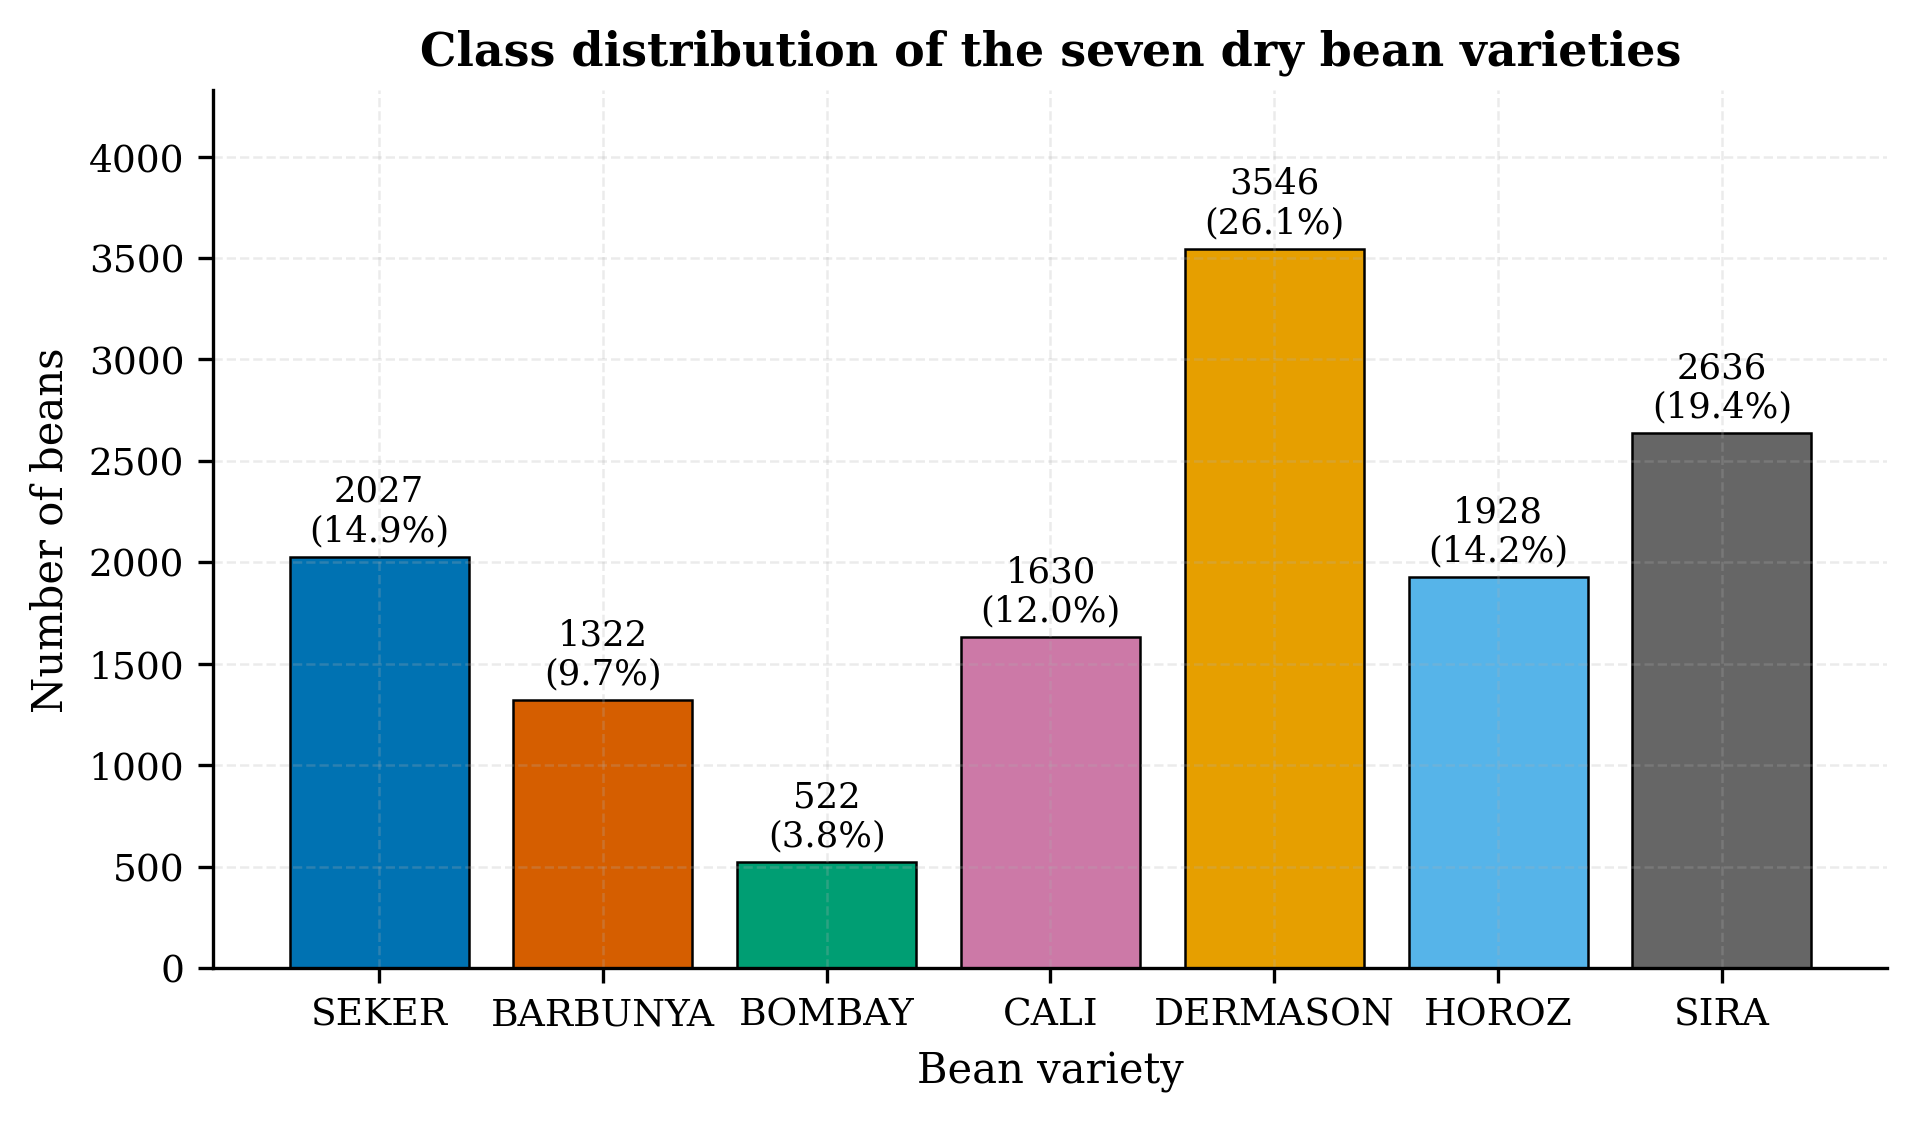
\includegraphics[width=0.70\textwidth]{fig_3_1_class_distribution.png}
\caption{Class distribution of the seven dry bean varieties. Counts and shares are
annotated; the smallest class, Bombay, supplies 3.84\% of the data.}
\label{fig:class_distribution}
\end{figure}

\subsection{Data completeness}

Every one of the 16 features is 100\% populated, as shown in
Figure~\ref{fig:missing}. There are also no infinite values, no negative values
and no constant columns. The completeness matters for the modelling stage: no
imputation is required, and the preprocessing pipeline therefore contains only a
scaler, which removes an entire class of leakage risks. A separate observation is
that \DuplicateRows{} rows are exact repeats of an earlier row across all 17
columns. They are discussed in Section~4.1 and were retained.

\begin{figure}[htbp]
\centering
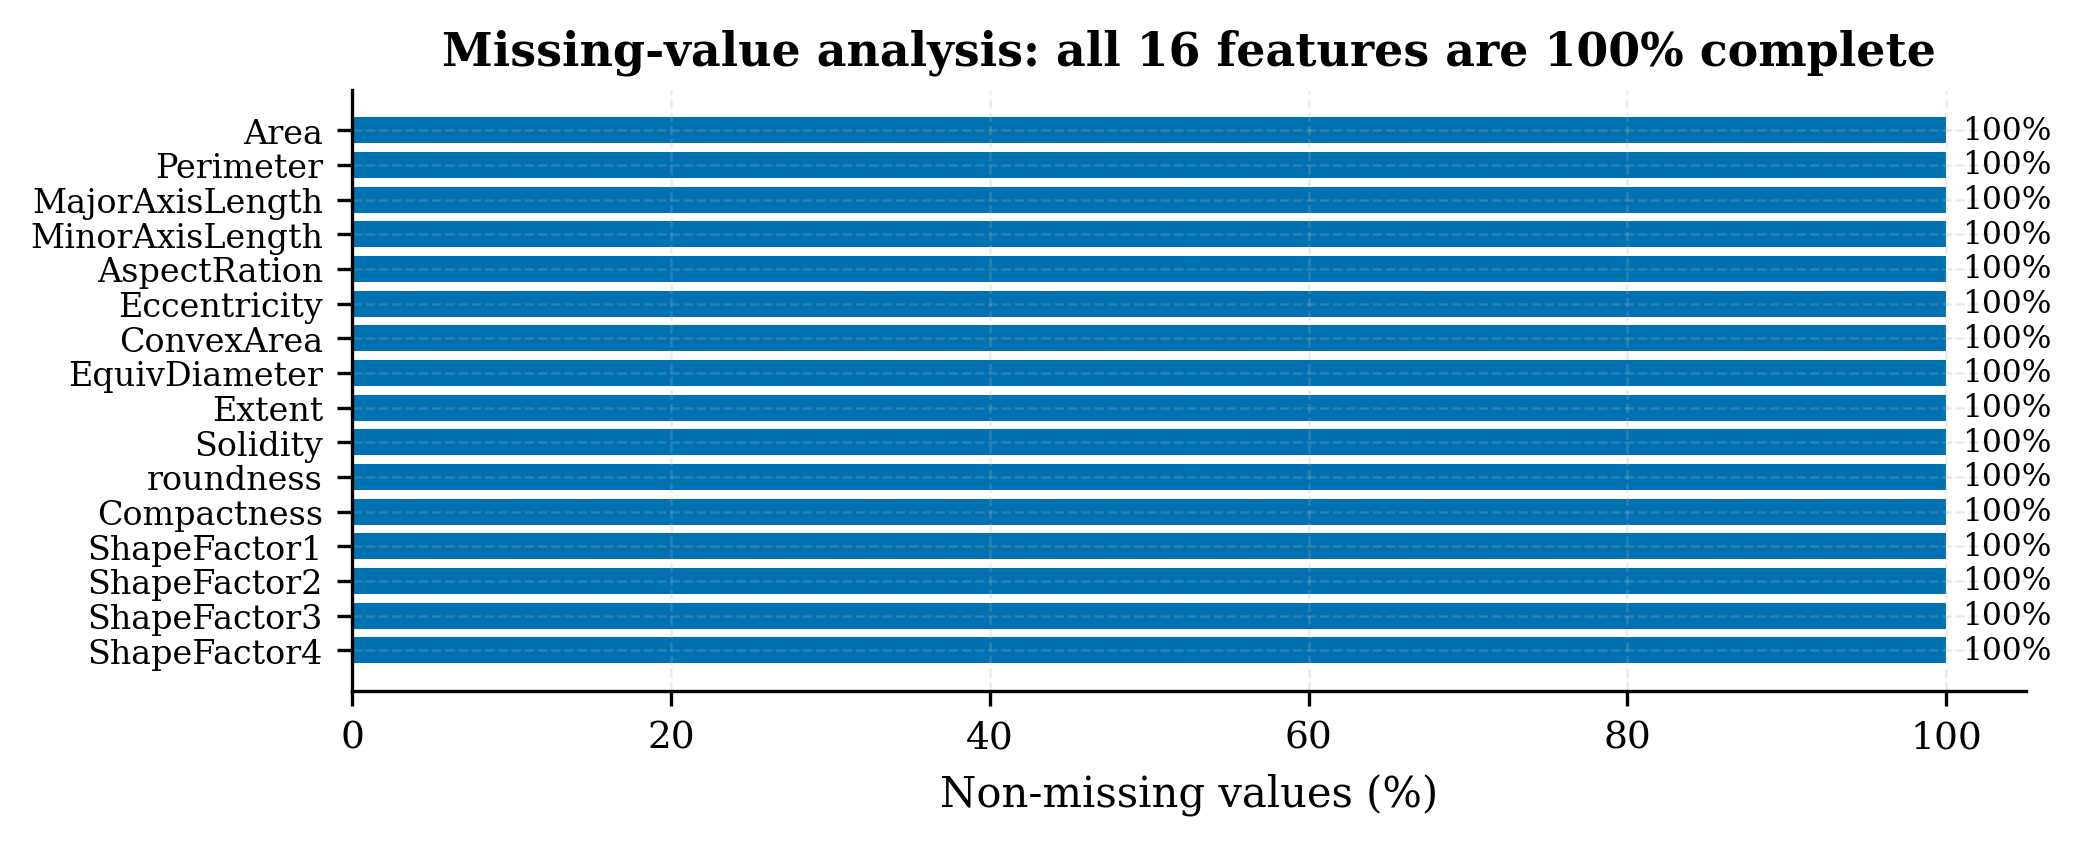
\includegraphics[width=0.60\textwidth]{fig_3_2_missing_values.png}
\caption{Missing-value analysis. All 16 features are complete, so no imputation
step is needed anywhere in the pipeline.}
\label{fig:missing}
\end{figure}

\subsection{Descriptive statistics}

Table~\ref{tab:descriptive} summarises the 16 features. Three properties govern
the preprocessing choices. The scales differ by four orders of magnitude:
\texttt{Area} has a mean of 53,048 pixels, while \texttt{ShapeFactor2} has a mean
of 0.002. Several features are strongly right-skewed (\texttt{Area} 2.95,
\texttt{ConvexArea} 2.94, \texttt{Solidity} $-$2.55, \texttt{ShapeFactor4}
$-$2.76), and the two bounded descriptors, \texttt{Solidity} and
\texttt{ShapeFactor4}, pile up against their upper limit. \texttt{Solidity} has a
standard deviation of 0.005, so almost all of its variance lies between 0.97 and
1.00.

\begin{table}[htbp]
\centering
\footnotesize
\caption{Descriptive statistics of the 16 morphological features (n = 13,611)}
\label{tab:descriptive}
\begin{tabular}{lrrrrrr}
\toprule
Feature & Mean & Std. dev. & Min & Median & Max & Skew \\
\midrule
Area & 5.305e+04 & 2.932e+04 & 2.042e+04 & 4.465e+04 & 2.546e+05 & 2.95 \\
Perimeter & 855.3 & 214.3 & 524.7 & 794.9 & 1985 & 1.63 \\
MajorAxisLength & 320.1 & 85.69 & 183.6 & 296.9 & 738.9 & 1.36 \\
MinorAxisLength & 202.3 & 44.97 & 122.5 & 192.4 & 460.2 & 2.24 \\
AspectRation & 1.583 & 0.2467 & 1.025 & 1.551 & 2.43 & 0.58 \\
Eccentricity & 0.7509 & 0.092 & 0.219 & 0.7644 & 0.9114 & -1.06 \\
ConvexArea & 5.377e+04 & 2.977e+04 & 2.068e+04 & 4.518e+04 & 2.633e+05 & 2.94 \\
EquivDiameter & 253.1 & 59.18 & 161.2 & 238.4 & 569.4 & 1.95 \\
Extent & 0.7497 & 0.0491 & 0.5553 & 0.7599 & 0.8662 & -0.90 \\
Solidity & 0.9871 & 0.0047 & 0.9192 & 0.9883 & 0.9947 & -2.55 \\
roundness & 0.8733 & 0.0595 & 0.4896 & 0.8832 & 0.9907 & -0.64 \\
Compactness & 0.7999 & 0.0617 & 0.6406 & 0.8013 & 0.9873 & 0.04 \\
ShapeFactor1 & 0.0066 & 0.0011 & 0.0028 & 0.0066 & 0.0105 & -0.53 \\
ShapeFactor2 & 0.0017 & 0.0006 & 0.0006 & 0.0017 & 0.0037 & 0.30 \\
ShapeFactor3 & 0.6436 & 0.099 & 0.4103 & 0.642 & 0.9748 & 0.24 \\
ShapeFactor4 & 0.9951 & 0.0044 & 0.9477 & 0.9964 & 0.9997 & -2.76 \\
\bottomrule
\end{tabular}
\end{table}


The practical consequence is that magnitude-based algorithms cannot consume these
columns raw: a Euclidean distance computed on unscaled values is, to within
rounding, a distance in \texttt{Area} alone. Section~4.2 addresses this with a
standard scaler inside a pipeline.

\subsection{Univariate distributions}

Figure~\ref{fig:histograms} shows all 16 histograms with their skewness. Three
groups are visible. The size features (\texttt{Area}, \texttt{Perimeter},
\texttt{ConvexArea}, \texttt{EquivDiameter} and the two axis lengths) are
right-skewed with a long upper tail, which is the signature of a mixture: the bulk
of the beans plus a small, distinctly larger group. The shape factors are
smoother and often bimodal. The bounded ratios (\texttt{Extent},
\texttt{Solidity}, \texttt{ShapeFactor4}) are concentrated near their ceilings.

The bimodality is not noise. It is the first indication that at least one variety
occupies a separate region of the size space, which the class-wise plots confirm.

\begin{figure}[htbp]
\centering
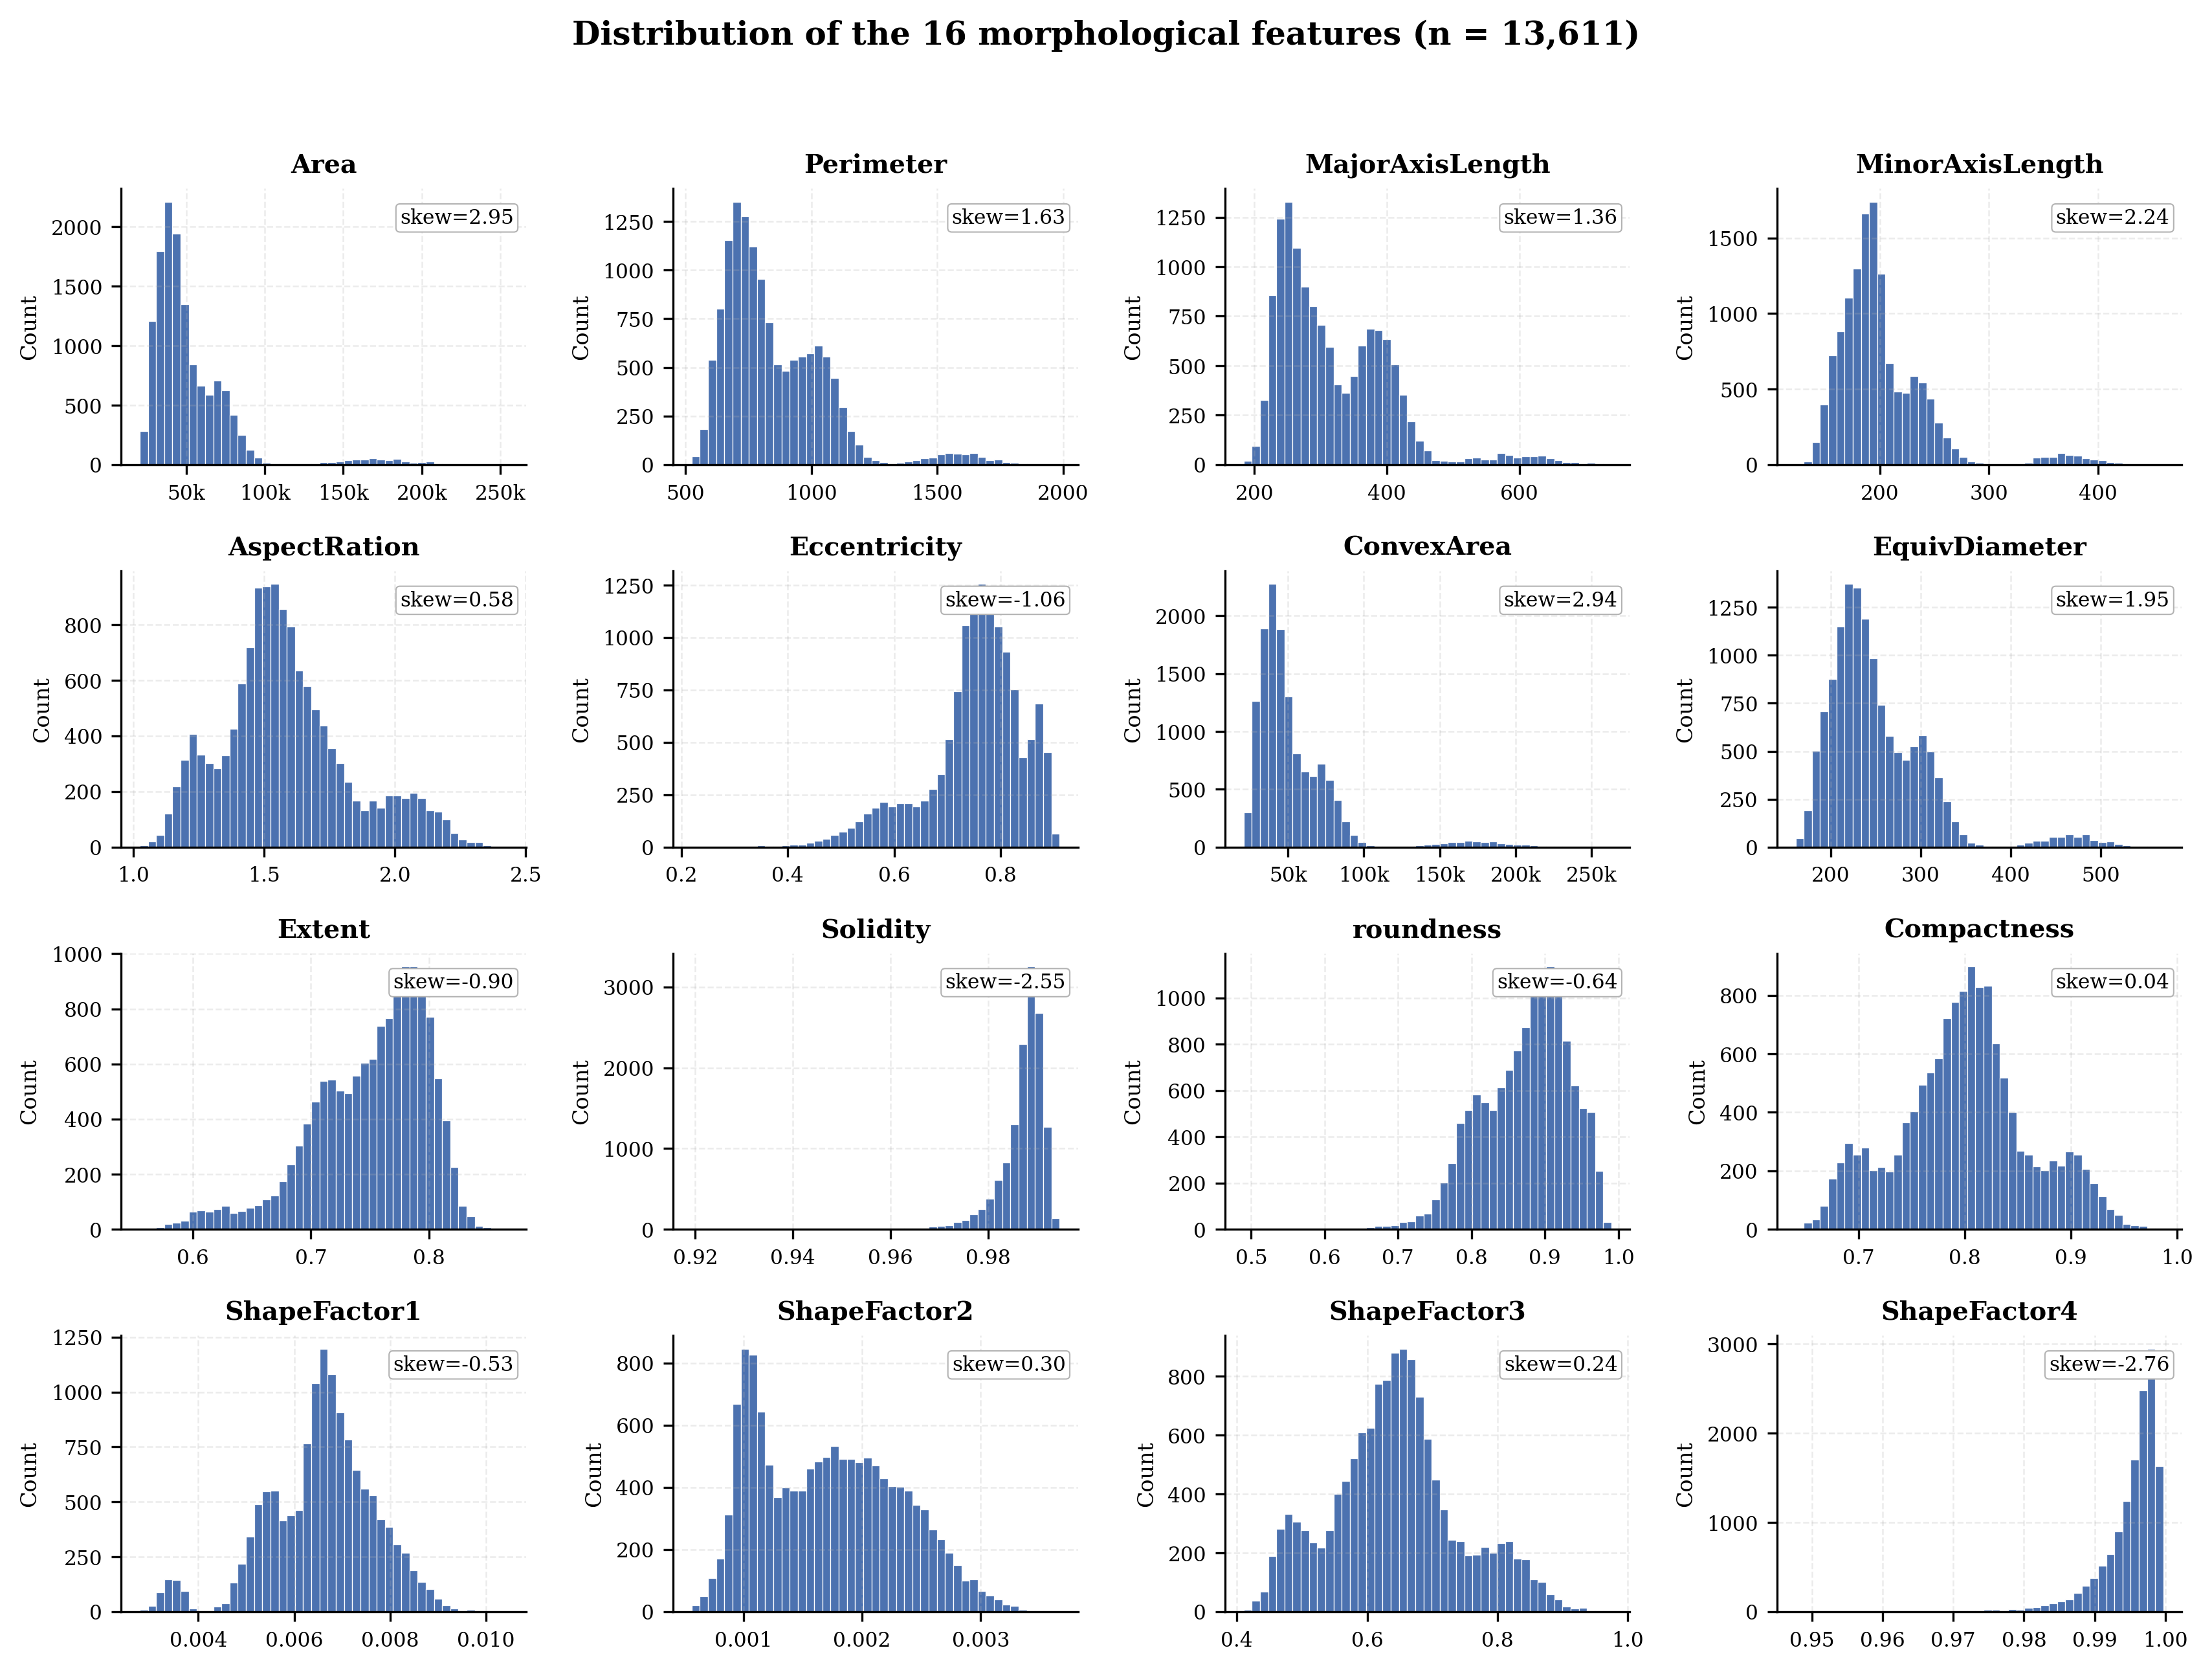
\includegraphics[width=0.95\textwidth]{fig_3_3_feature_histograms.png}
\caption{Distribution of the 16 morphological features. Skewness is annotated in
each panel. Size features are right-skewed; several shape factors are bimodal.}
\label{fig:histograms}
\end{figure}

\subsection{Class-wise distributions}

Figure~\ref{fig:boxplots} breaks eight features down by variety, and
Figure~\ref{fig:violin} shows the density of four of them. The separation is
uneven. \texttt{Area} isolates Bombay completely: its mean area of 173,485
pixels is 2.4 times that of Barbunya, the next largest, and no other variety
reaches its lower quartile. Dermason is the smallest at 32,119 pixels. The
remaining five varieties form a band between roughly 39,000 and 76,000 pixels
where the ranges overlap almost completely.

Shape separates what size cannot. Seker is the roundest variety
(\texttt{roundness} mean 0.945, \texttt{Compactness} 0.897, eccentricity 0.585),
while Horoz is the most elongated (\texttt{Compactness} 0.701, eccentricity
0.867, \texttt{Extent} 0.706). Cali and Barbunya have similar areas (75,538 and
69,804 pixels) but differ in compactness (0.757 against 0.805), which is exactly
the kind of distinction that a classifier must learn from a ratio rather than
from a magnitude.

\begin{figure}[htbp]
\centering
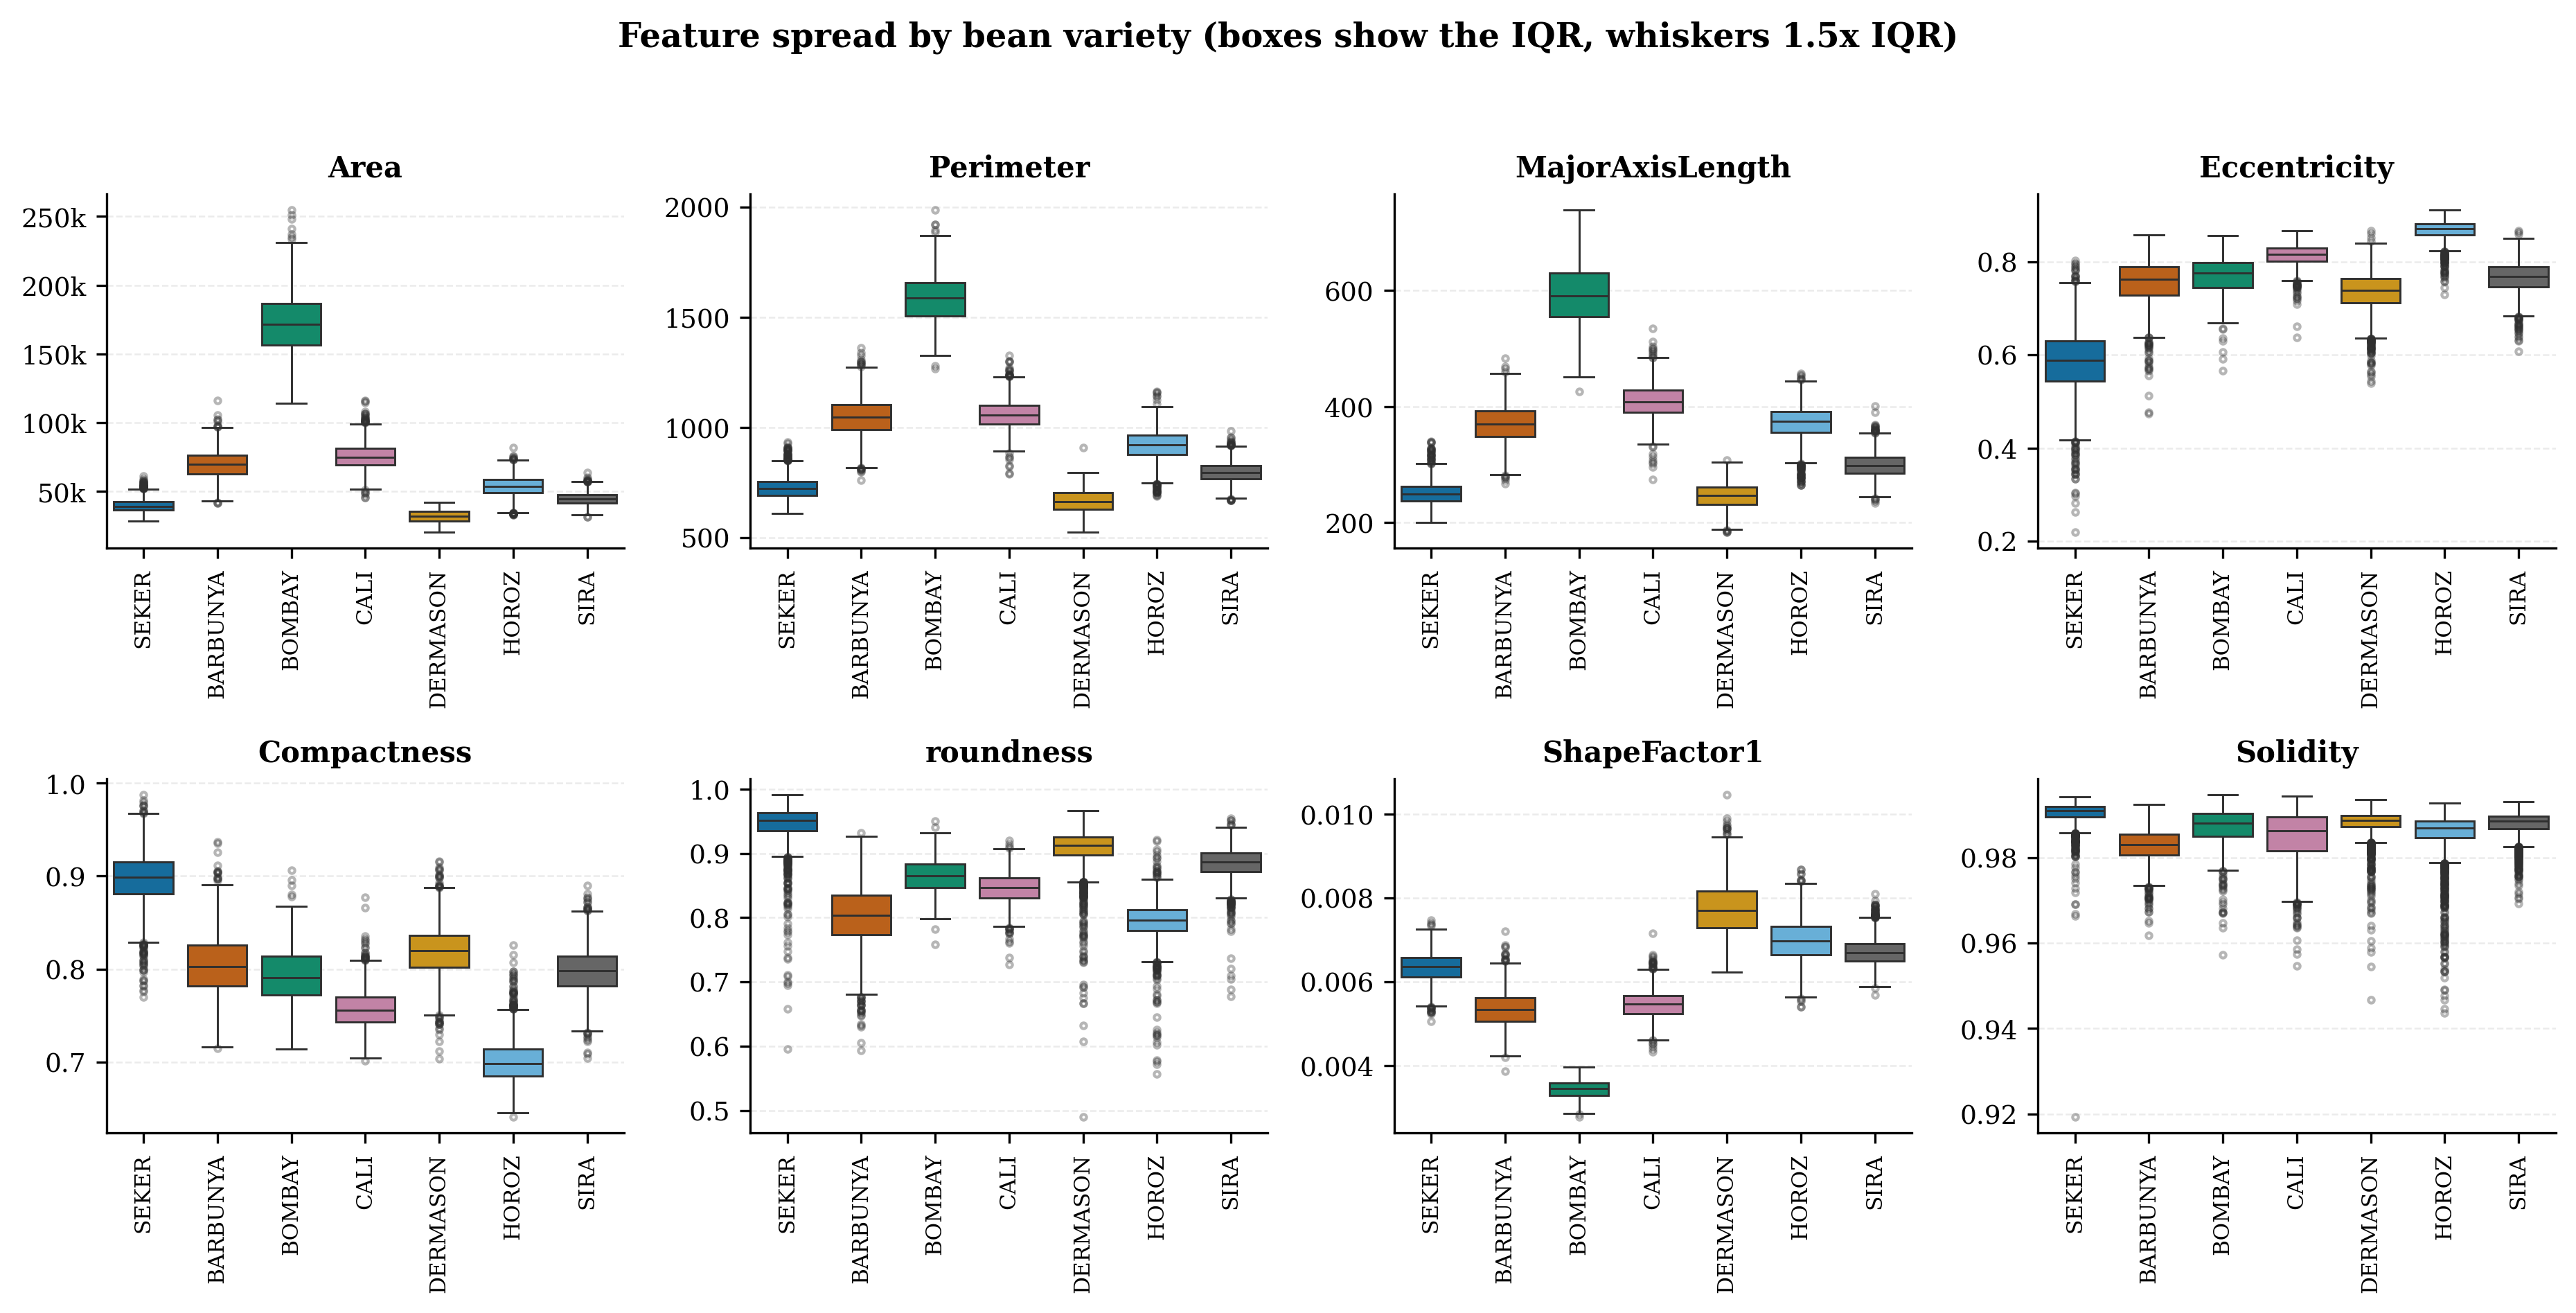
\includegraphics[width=0.95\textwidth]{fig_3_4_boxplots_by_class.png}
\caption{Feature spread by variety. Bombay is separated by every size feature;
the other six overlap and require shape information.}
\label{fig:boxplots}
\end{figure}

\begin{figure}[htbp]
\centering
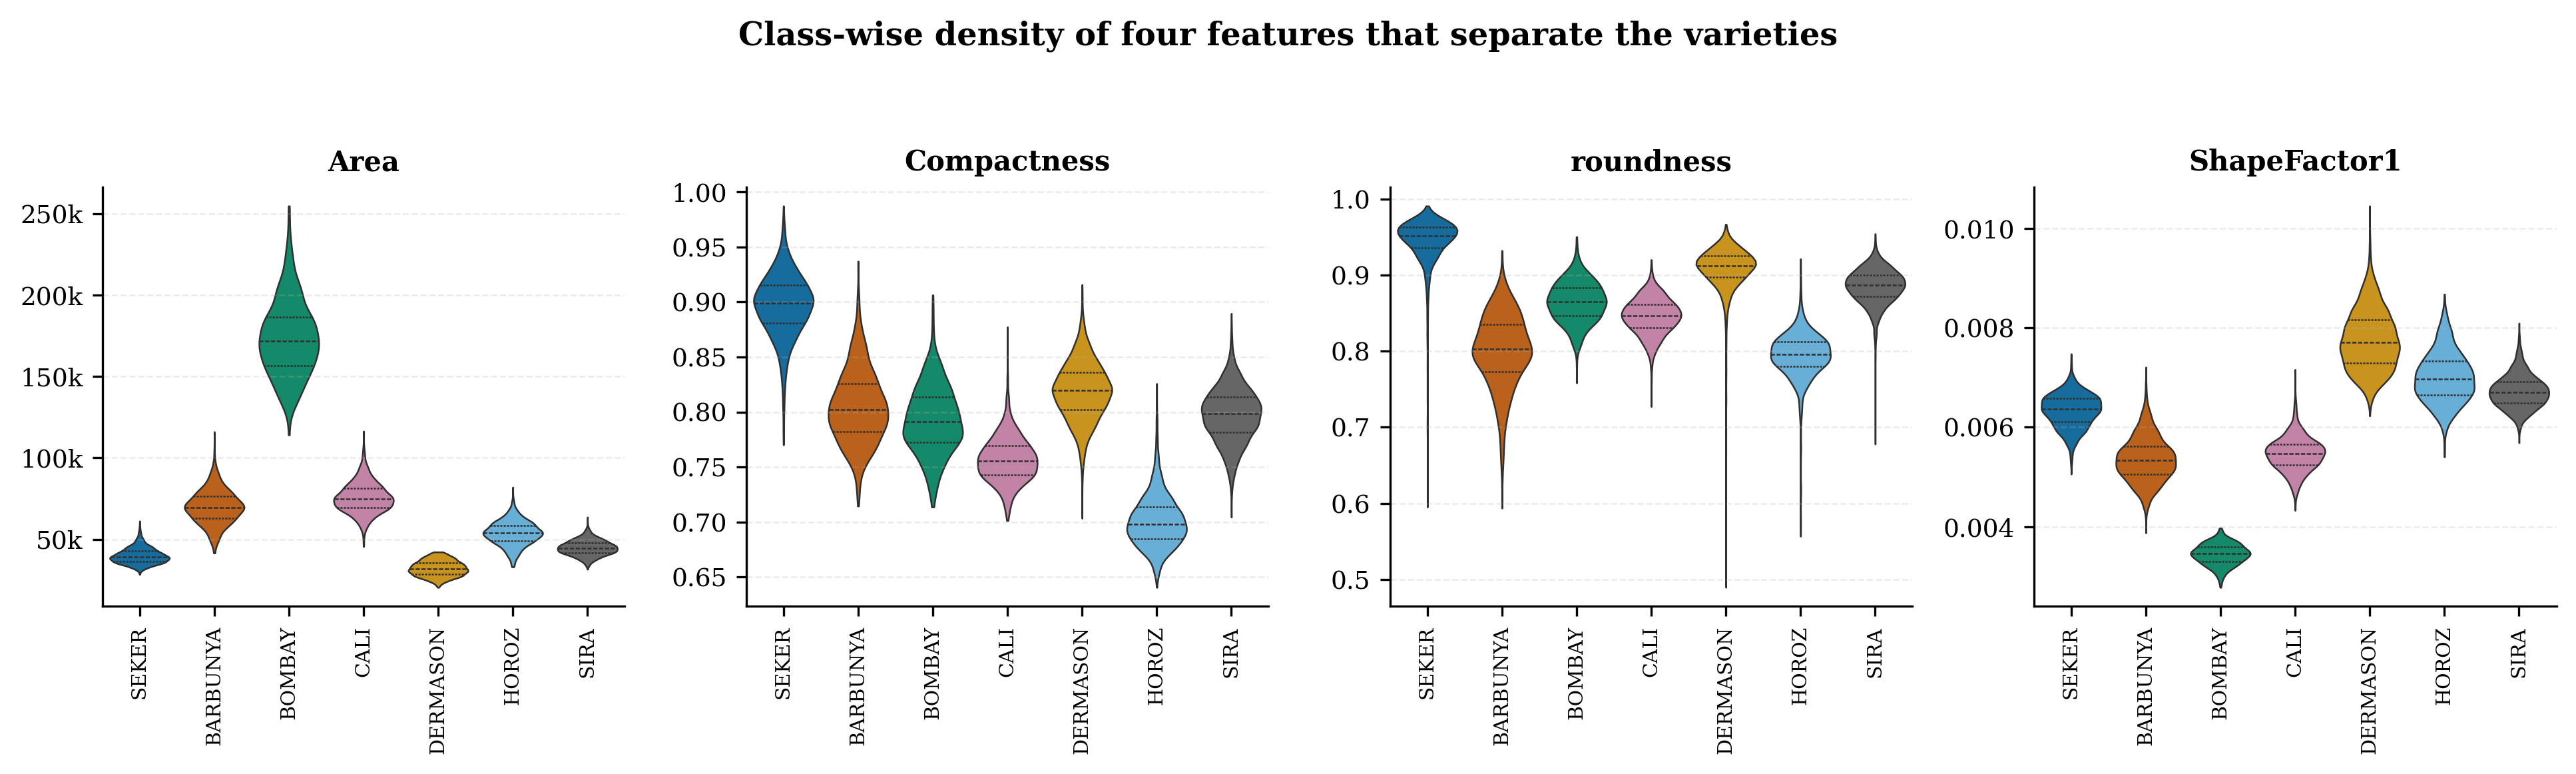
\includegraphics[width=0.90\textwidth]{fig_3_7_classwise_comparison.png}
\caption{Class-wise density of four informative features. Seker concentrates at
high roundness, Horoz at low compactness, and Bombay sits alone at low
ShapeFactor1.}
\label{fig:violin}
\end{figure}

\subsection{Correlation structure}

Figure~\ref{fig:corr} is the Pearson correlation matrix and
Table~\ref{tab:corr_pairs} lists the ten strongest pairs. Twenty-one pairs exceed
$|r| = 0.90$. \texttt{Area} and \texttt{ConvexArea} are effectively the same
variable ($r = 0.9999$), which is expected because a bean is nearly convex and
its convex hull therefore covers almost the same pixels. \texttt{Compactness} and
\texttt{ShapeFactor3} reach $-0.9987$, and \texttt{Perimeter} correlates with
\texttt{EquivDiameter} at 0.9914.

Two decisions follow. First, the multicollinearity is real and will affect the
interpretation of feature importance: when two columns carry the same
information, an impurity-based or permutation-based importance can split the
credit arbitrarily between them. Chapter~6 reports this caveat with the results
rather than ignoring it. Second, the correlation is \emph{not} treated as a reason
to delete columns. A tree ensemble can still exploit the small residual
difference between \texttt{Area} and \texttt{ConvexArea}, and the ablation in
Section~6.4 measures the cost of removing the redundant cluster instead of
assuming it.

\begin{figure}[htbp]
\centering
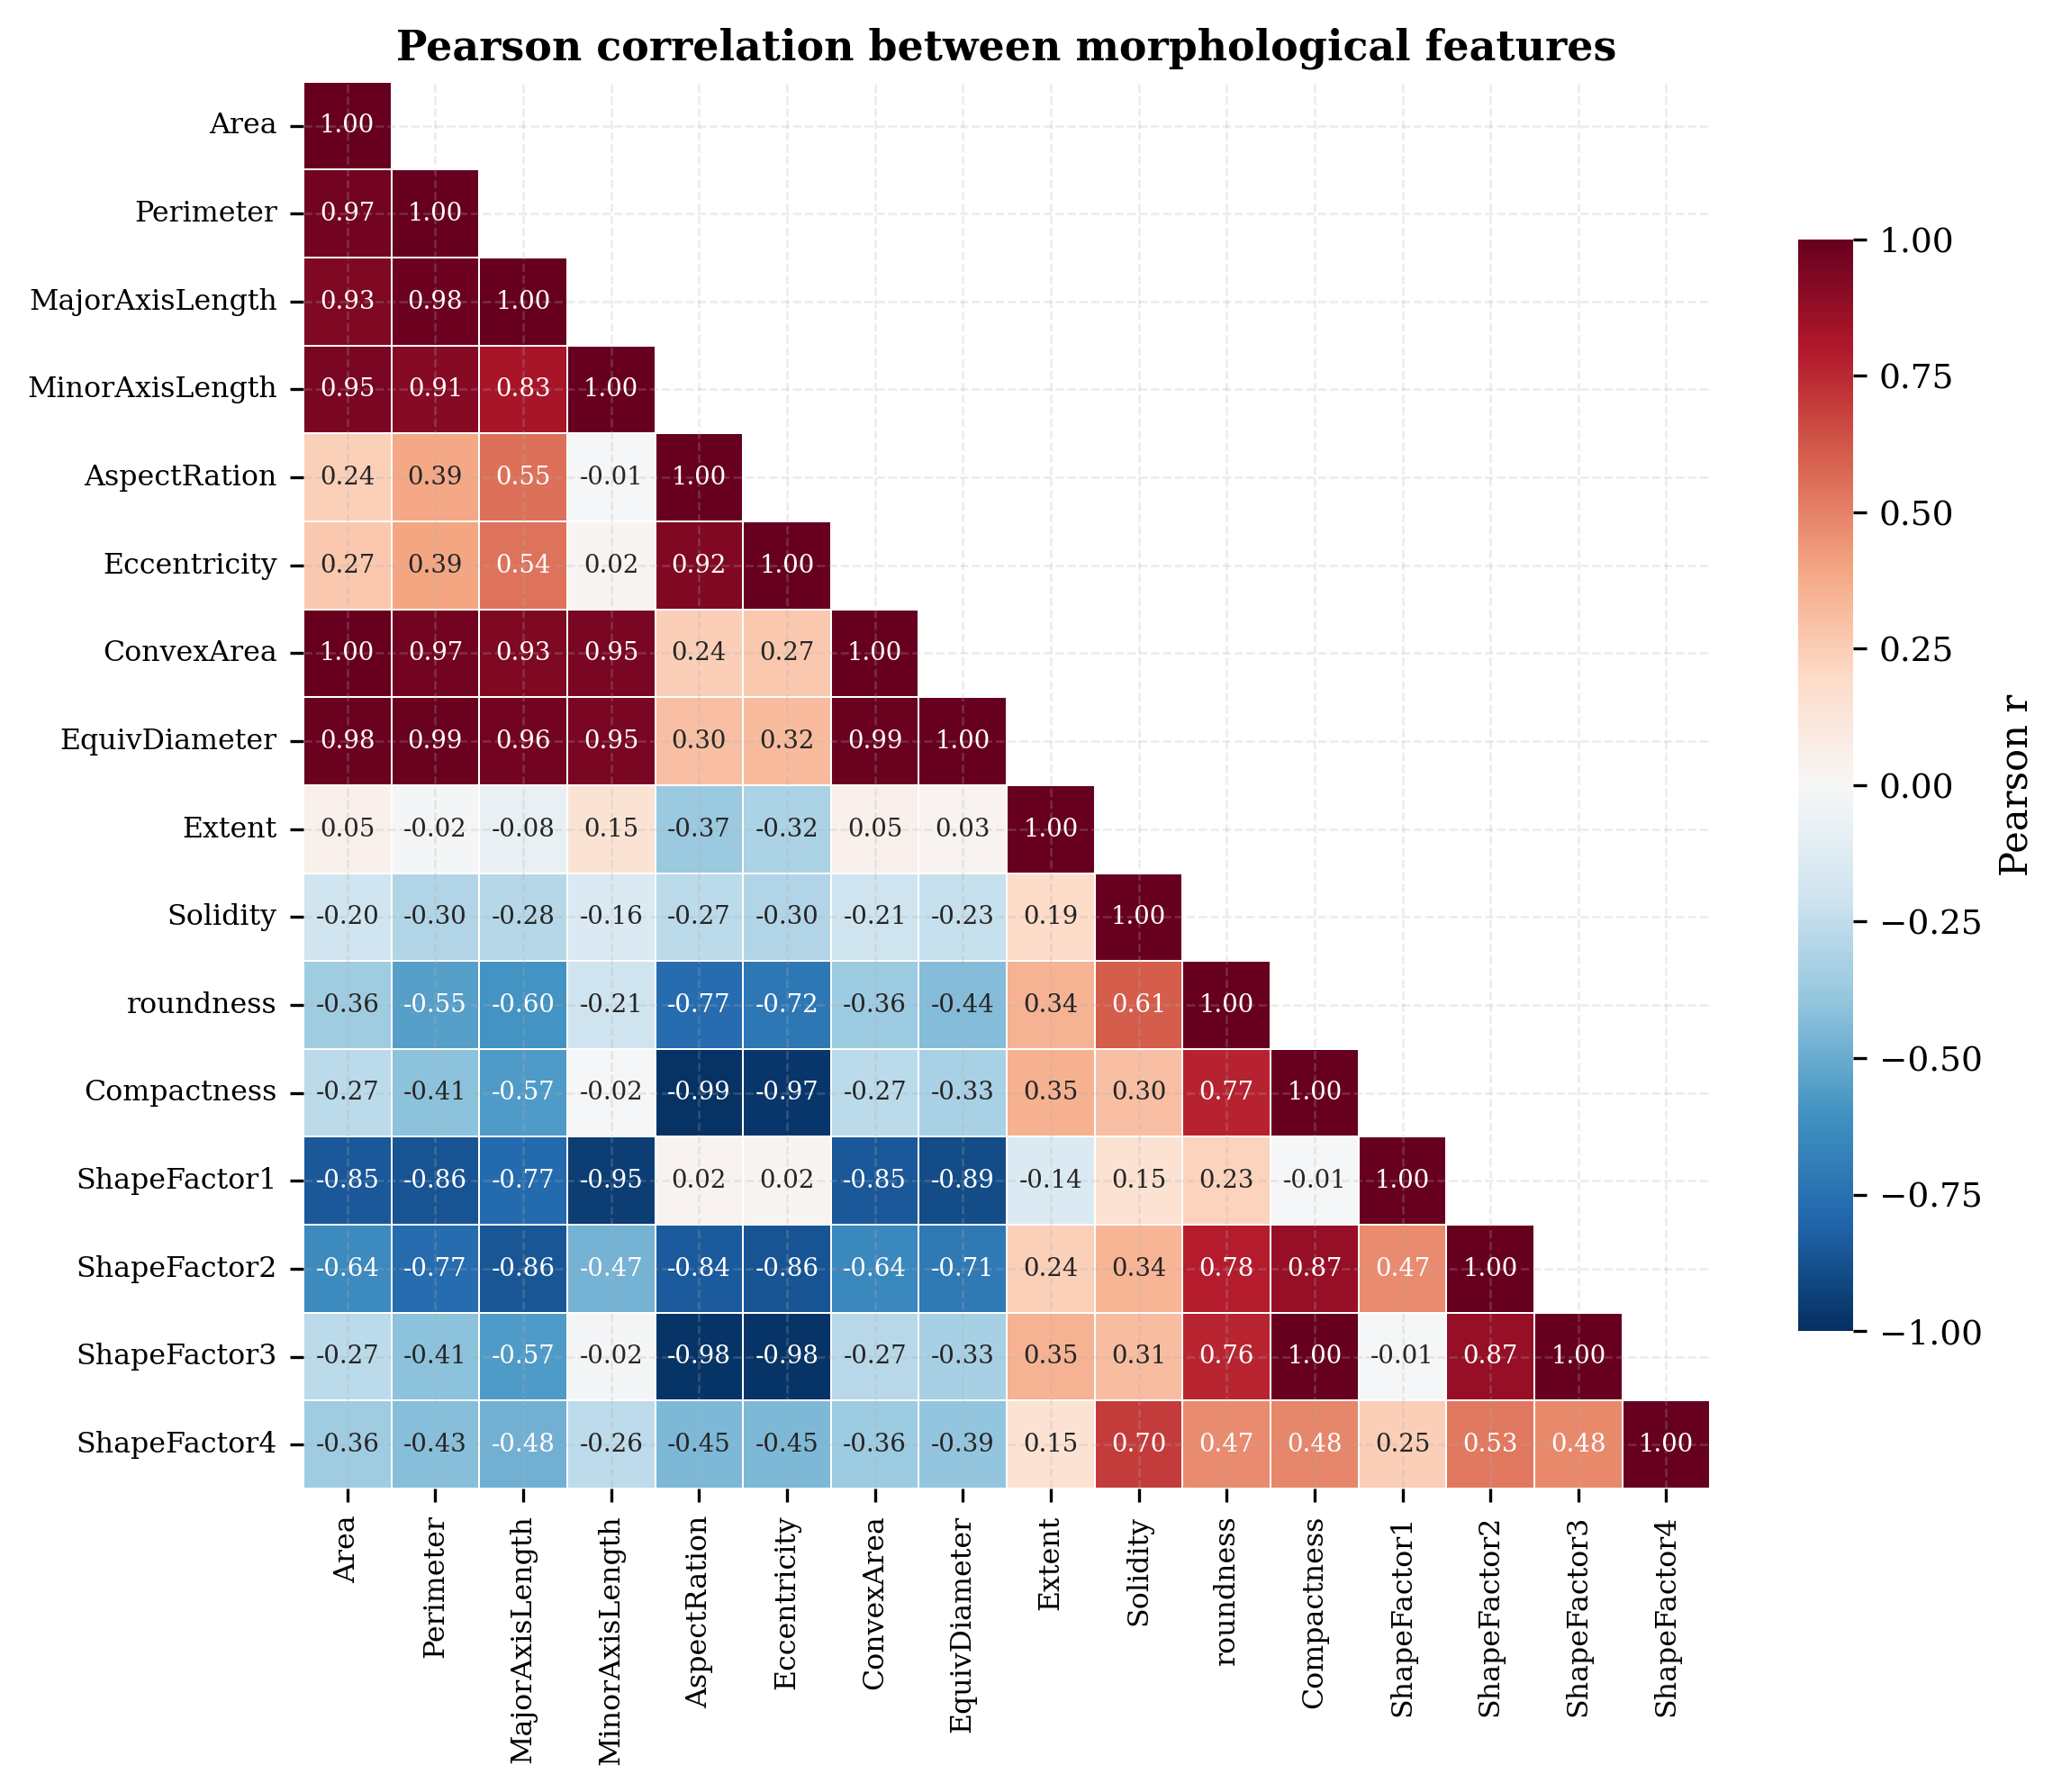
\includegraphics[width=0.62\textwidth]{fig_3_5_correlation_heatmap.png}
\caption{Pearson correlation between the 16 features. The lower triangle is shown;
21 pairs exceed $|r| = 0.90$.}
\label{fig:corr}
\end{figure}

\begin{table}[htbp]
\centering
\small
\caption{The ten strongest feature correlations (all 21 pairs above 0.90 are listed in Appendix B)}
\label{tab:corr_pairs}
\begin{tabular}{lr}
\toprule
Feature pair & Pearson r \\
\midrule
Area -- ConvexArea & +0.9999 \\
Compactness -- ShapeFactor3 & +0.9987 \\
Perimeter -- EquivDiameter & +0.9914 \\
AspectRation -- Compactness & -0.9877 \\
ConvexArea -- EquivDiameter & +0.9852 \\
Area -- EquivDiameter & +0.9850 \\
Eccentricity -- ShapeFactor3 & -0.9811 \\
AspectRation -- ShapeFactor3 & -0.9786 \\
Perimeter -- MajorAxisLength & +0.9773 \\
Eccentricity -- Compactness & -0.9703 \\
\bottomrule
\end{tabular}
\end{table}


\subsection{Multivariate relationships}

The pair plot in Figure~\ref{fig:pairplot} is the clearest single view of the
problem. Bombay forms an isolated cluster at high area and high perimeter.
Dermason forms a second, low-area cluster. The remaining five varieties occupy one
dense cloud whose internal structure is weak: Cali and Barbunya overlap almost
completely, and Sira sits between them and Dermason. Figure~\ref{fig:scatter}
shows the same structure in two dimensions and makes the practical consequence
visible: \texttt{Area} against \texttt{Perimeter} is nearly a straight line,
because both measure size, whereas \texttt{Compactness} against \texttt{roundness}
is the plane in which the five overlapping varieties actually differ.

Two adjacencies are visible inside the cloud and both matter later. Cali
(mean area 75,538, compactness 0.757) and Barbunya (69,804, 0.805) occupy the same
size band and differ mainly in how elongated they are. Dermason (32,119, 0.819)
and Sira (44,729, 0.797) are neighbours in both size and compactness, and their
roundness values, 0.908 and 0.885, are closer than any other pair except
Cali--Barbunya.

This is the observation that determines the model expectations. Any reasonable
classifier should score close to 1.00 on Bombay, whose area separates it from
everything else by a wide margin, and the ranking of the models will be decided by
the beans that sit in those two adjacent pairs. Chapter~6 tests that expectation
rather than assuming it.

\begin{figure}[htbp]
\centering
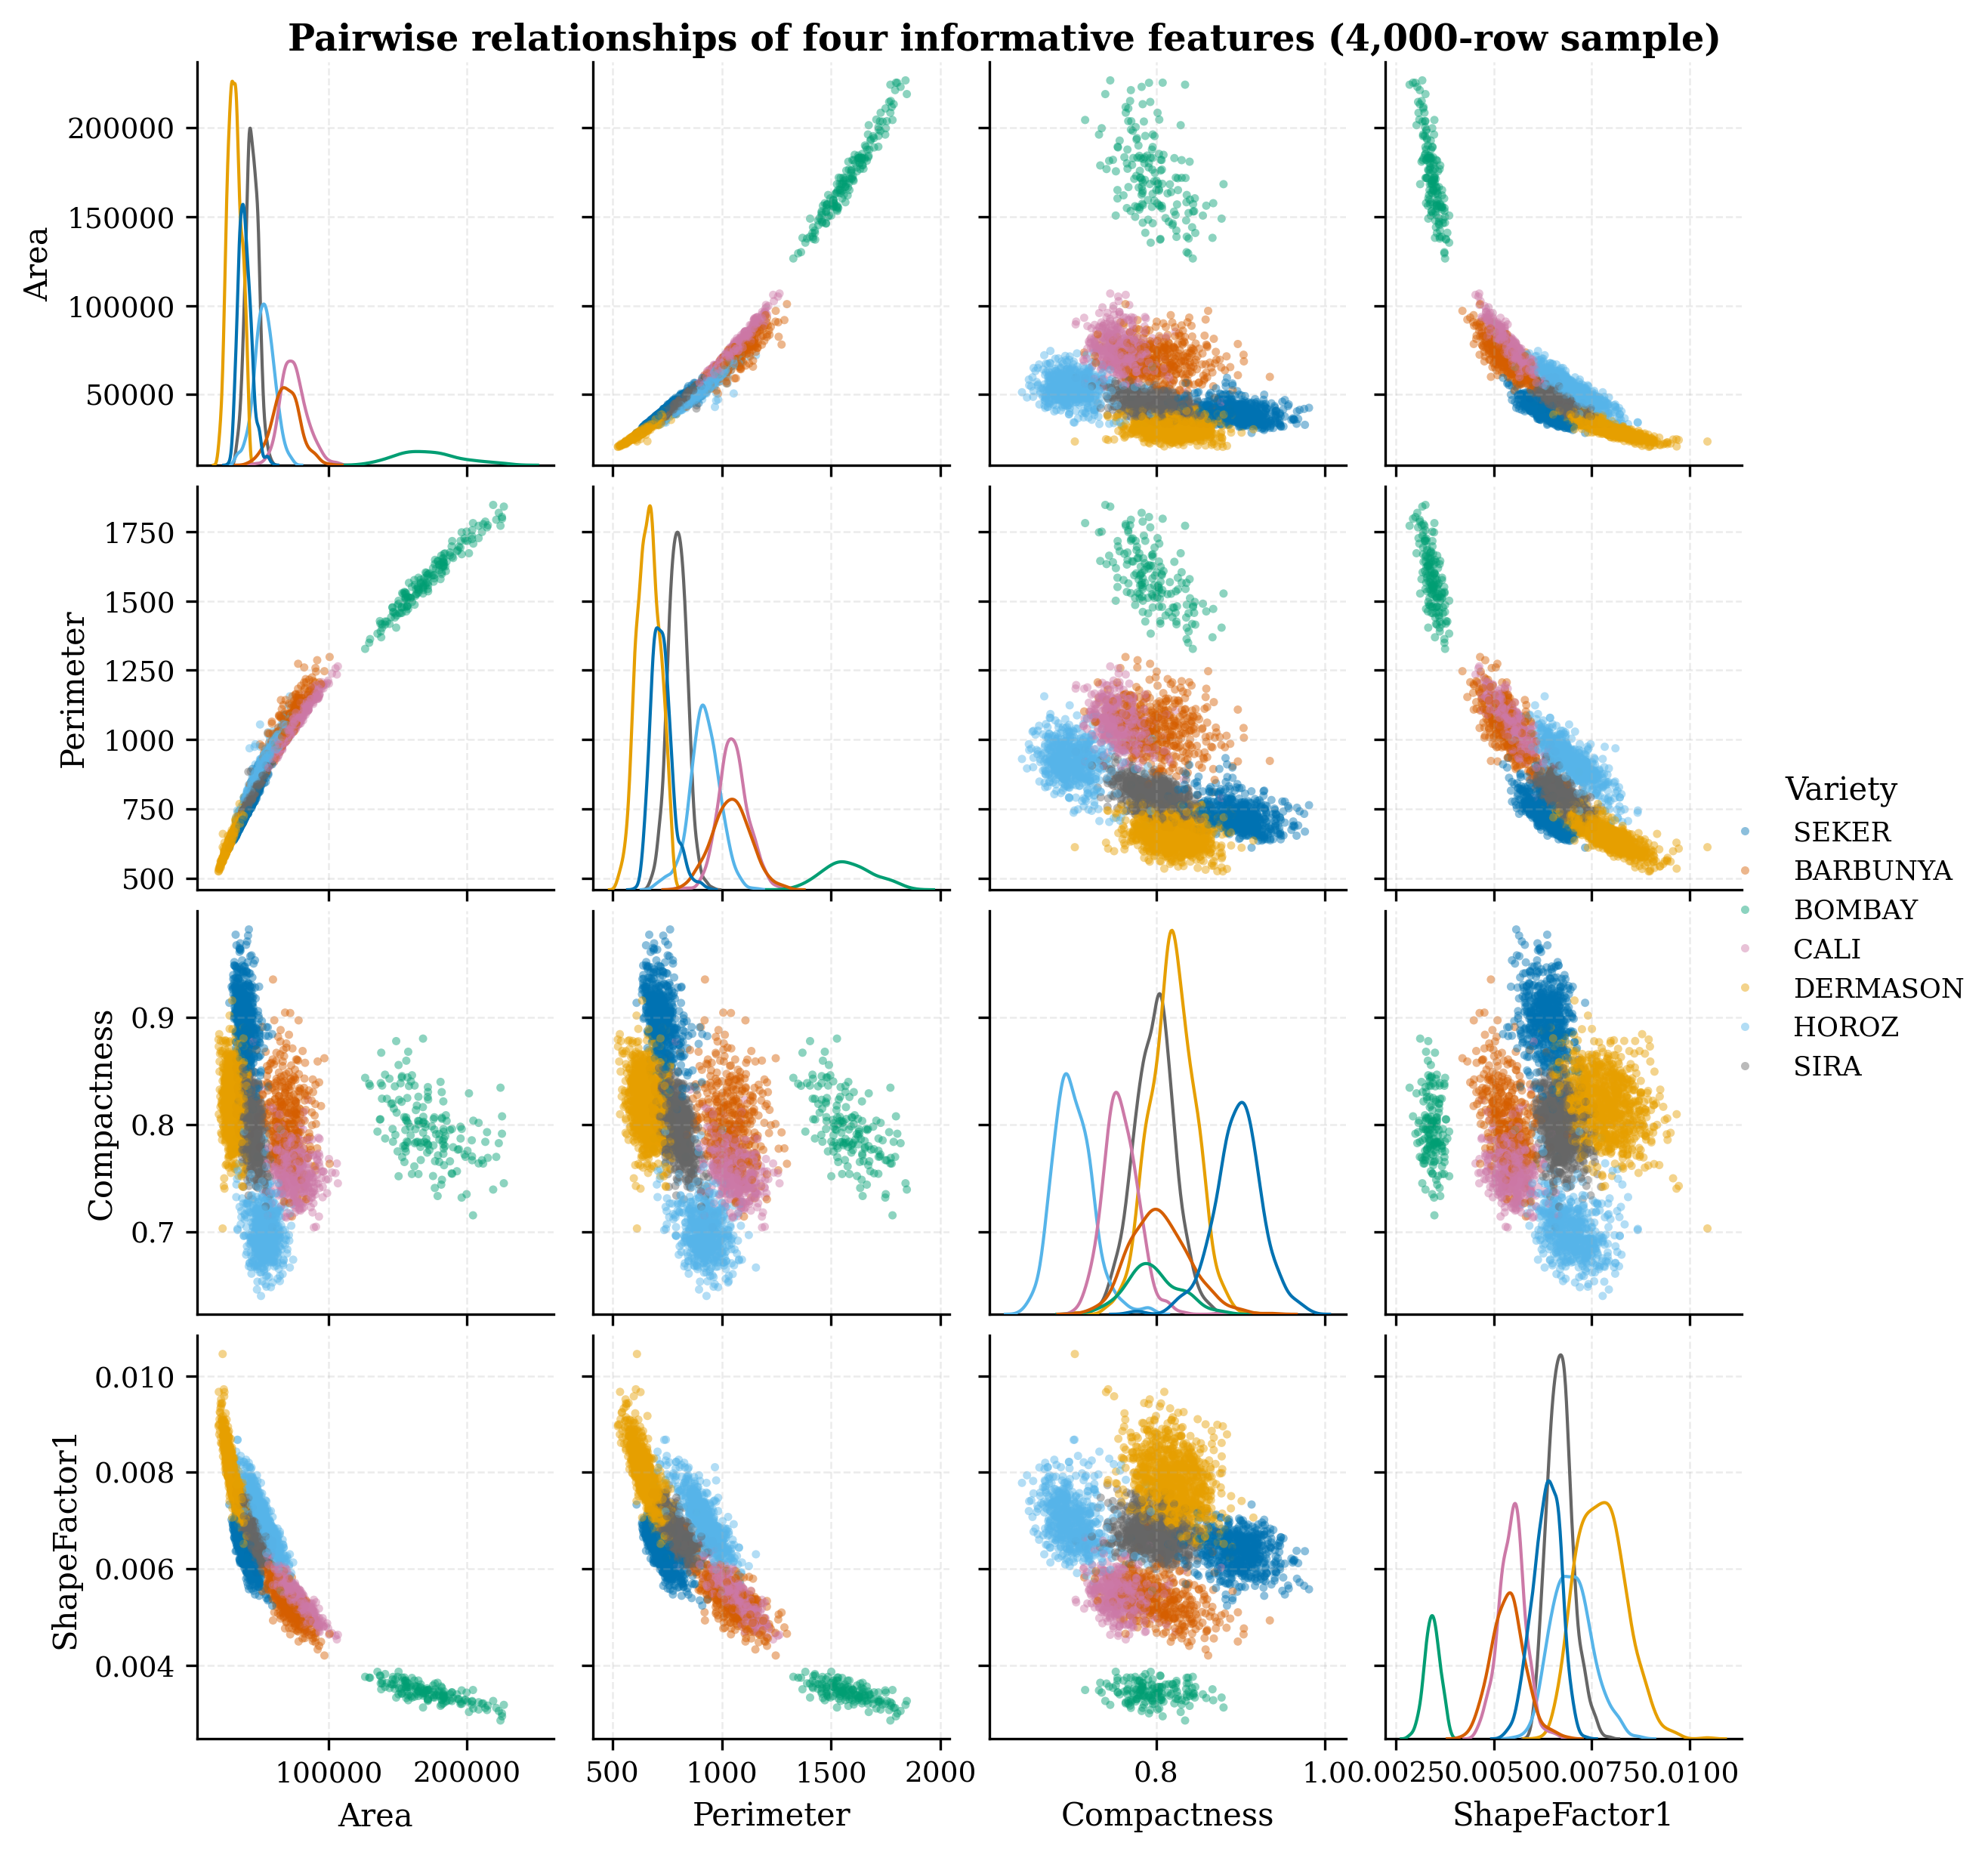
\includegraphics[width=0.62\textwidth]{fig_3_6_pairplot.png}
\caption{Pairwise relationships of four informative features on a 4,000-bean
sample. Two varieties separate cleanly; five overlap in a single cloud.}
\label{fig:pairplot}
\end{figure}

\begin{figure}[htbp]
\centering
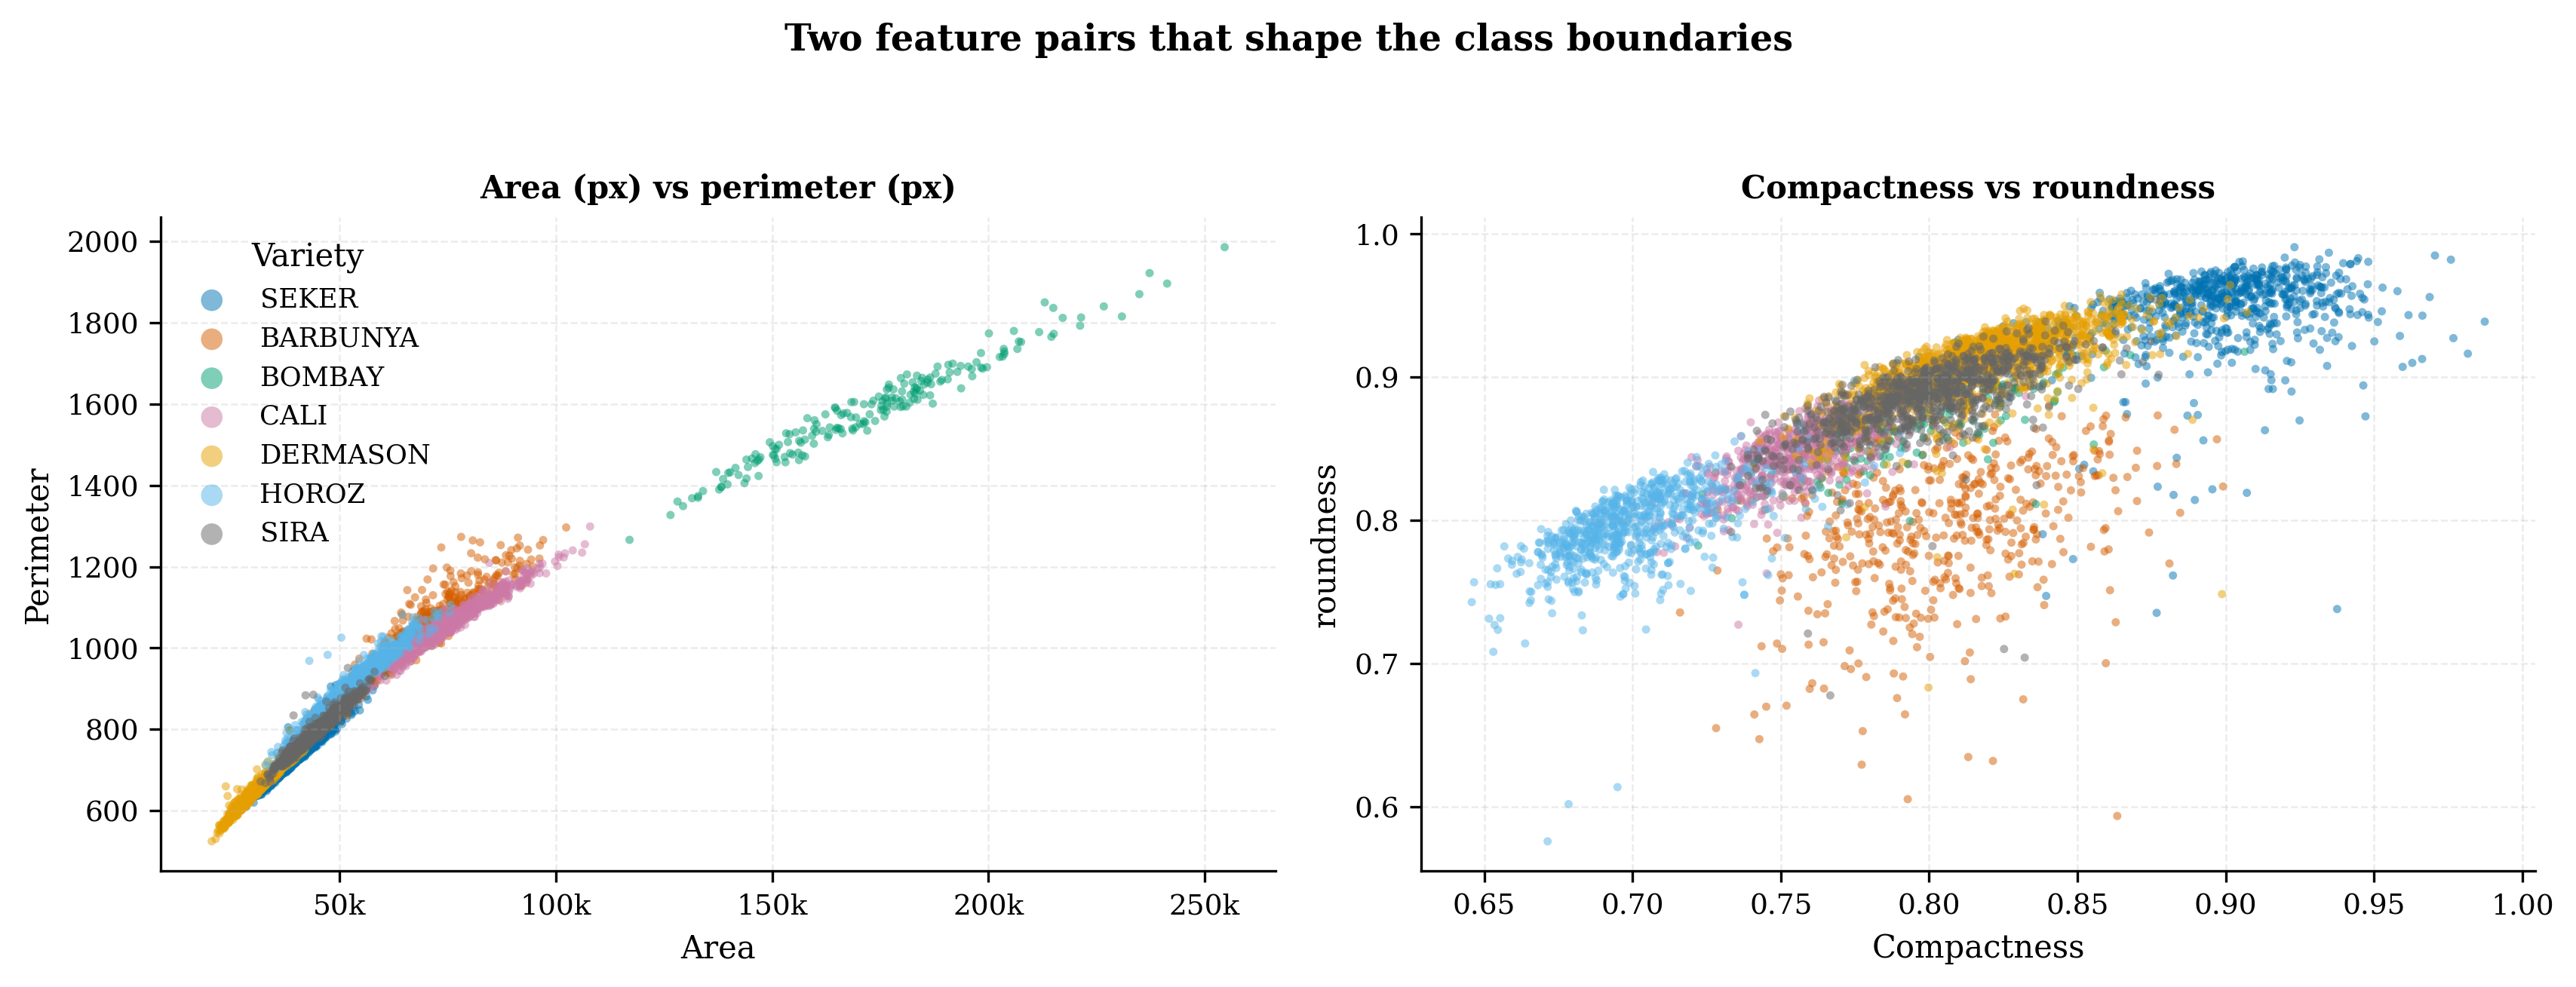
\includegraphics[width=0.92\textwidth]{fig_3_8_scatter_relationships.png}
\caption{Two feature pairs. Area and perimeter are almost collinear, so they
encode size twice; compactness and roundness separate the overlapping varieties.}
\label{fig:scatter}
\end{figure}

\subsection{Outliers}

Tukey's rule with a 1.5 IQR fence flags between 91 (\texttt{roundness}) and 843
(\texttt{Eccentricity}) observations per feature; Figure~\ref{fig:outliers} shows
the counts and the standardised spread. Almost all flagged points are large beans,
which belong to Bombay, rather than implausible measurements. No value falls
outside the physical range implied by the imaging setup, and there is no evidence
of a data-entry error: the size features are internally consistent
($\text{Area} \approx \pi E_d^2/4$ holds throughout).

Removing them would therefore delete the variety that is easiest to classify and
would bias the model against large beans. The outliers were retained. This is a
deliberate decision, not an oversight, and it is revisited as a limitation in
Section~7.2: a model trained without them would be less able to recognise an
unusually large Seker, but also less likely to mistake a Bombay for something
else.

\begin{figure}[htbp]
\centering
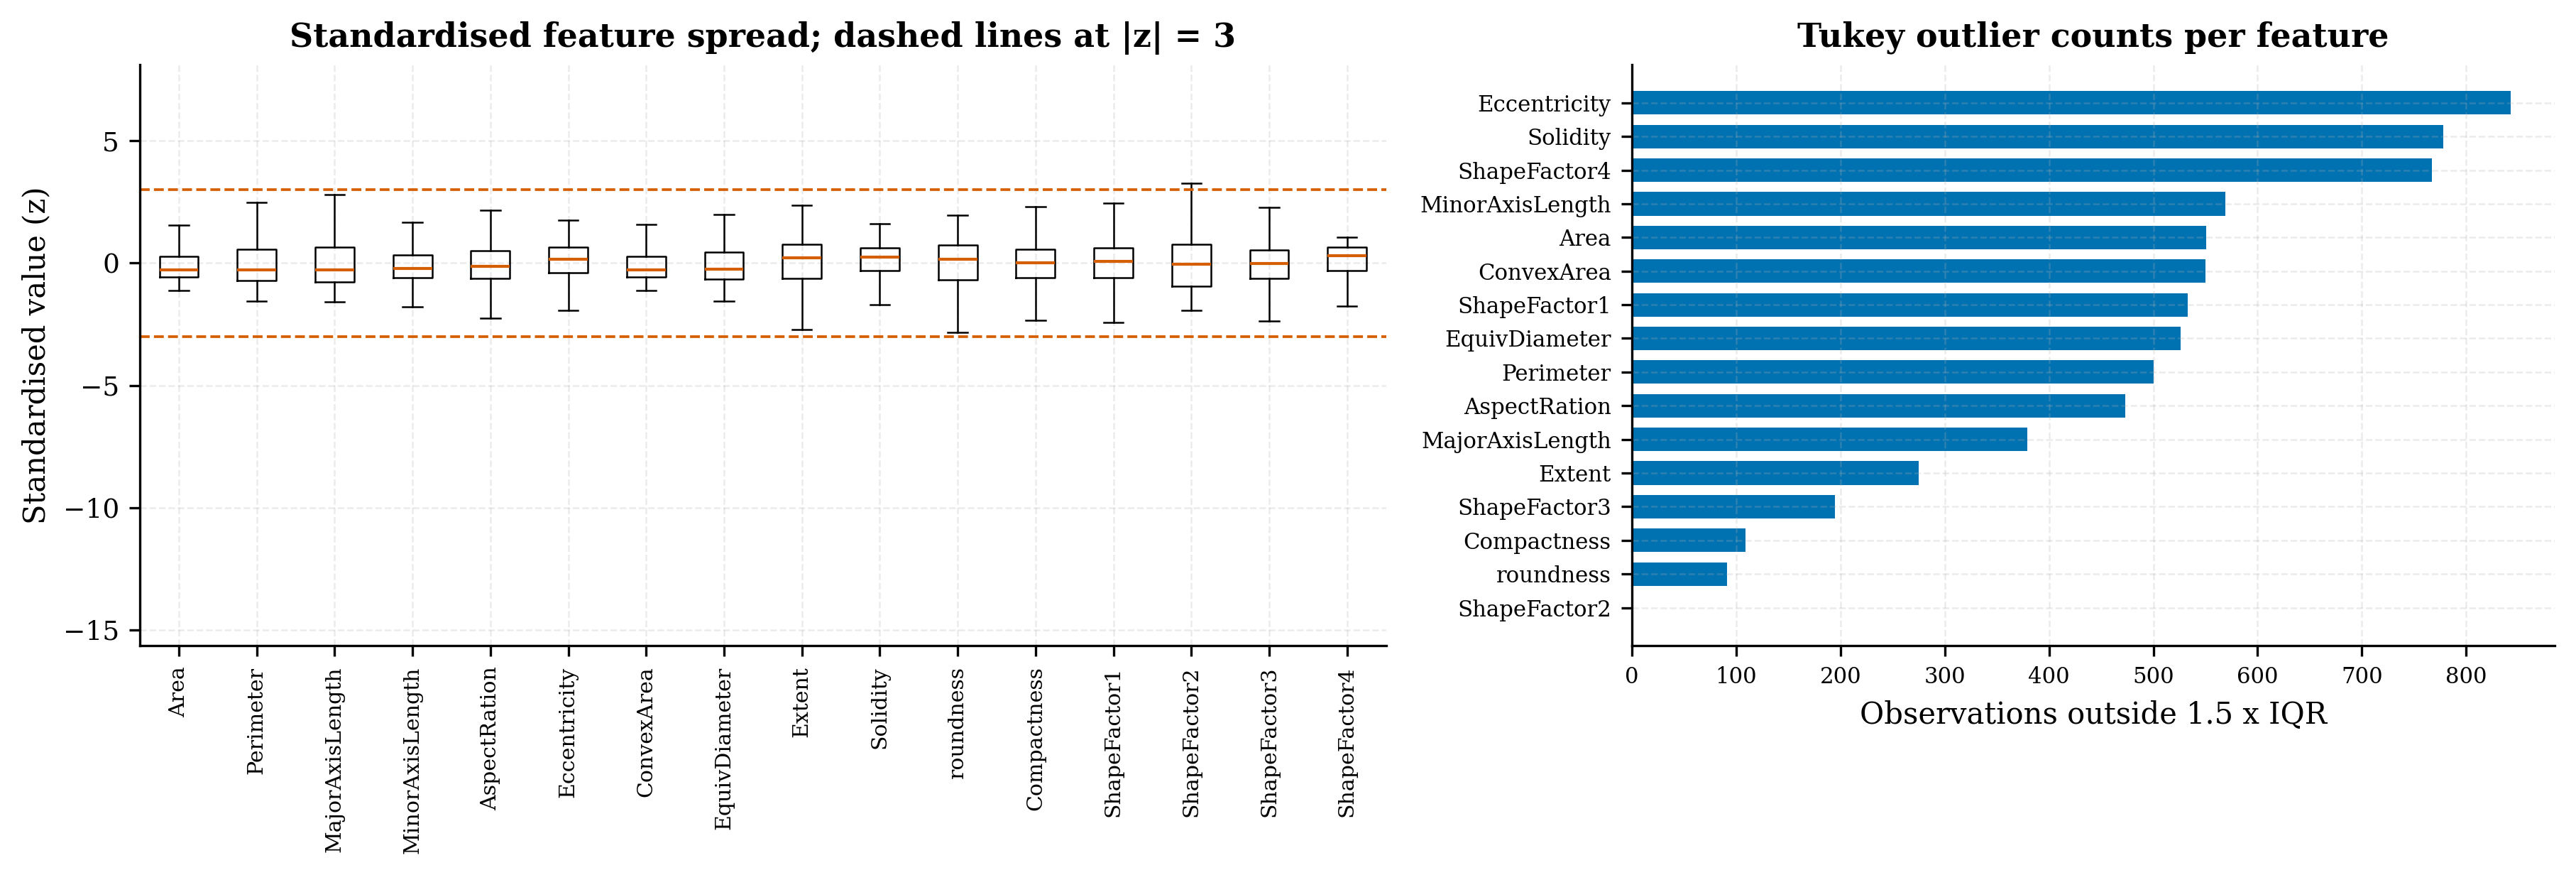
\includegraphics[width=0.92\textwidth]{fig_3_9_outlier_analysis.png}
\caption{Outlier analysis. Left: standardised spread with $\pm 3$ reference lines.
Right: Tukey outlier counts per feature. Flagged points are genuine large beans,
not measurement errors.}
\label{fig:outliers}
\end{figure}

\subsection{Discriminative power}

Figure~\ref{fig:anova} ranks the features by a one-way ANOVA $F$-statistic
computed across the seven classes. This is a descriptive statistic about the data,
not a model output, and it is used only to decide which features deserve a
dedicated plot. The size features lead, which is expected given Bombay, followed
by \texttt{ShapeFactor1} and \texttt{Compactness}. \texttt{Solidity} and
\texttt{ShapeFactor4} rank last, consistent with their narrow ranges.

\begin{figure}[htbp]
\centering
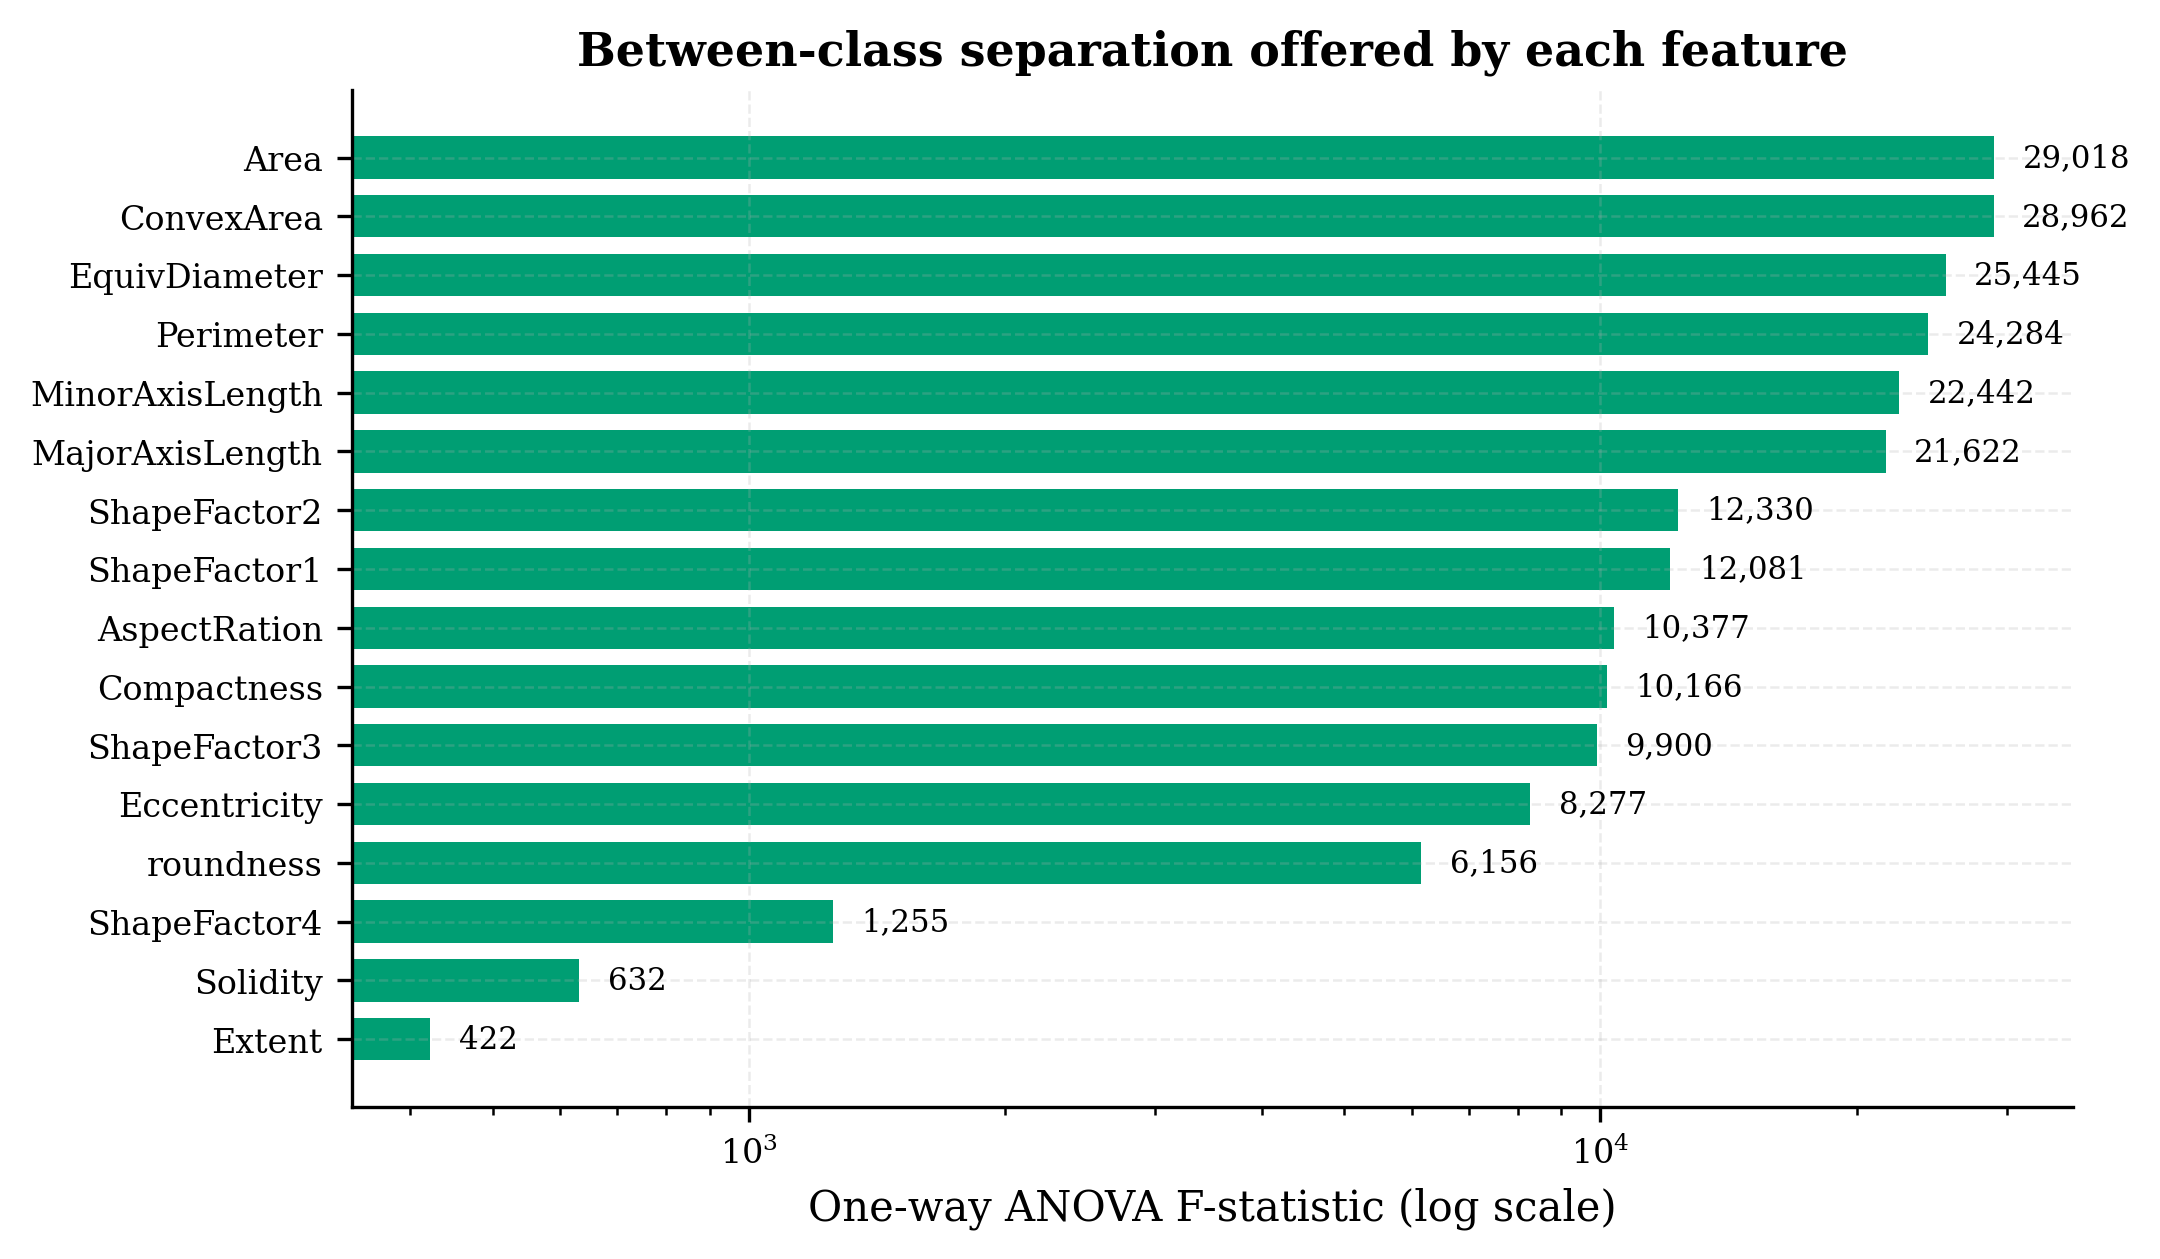
\includegraphics[width=0.66\textwidth]{fig_3_10_discriminative_power.png}
\caption{Between-class separation offered by each feature, measured by a one-way
ANOVA $F$-statistic on a logarithmic scale.}
\label{fig:anova}
\end{figure}

\section{Observations from EDA}

Six observations carried into the modelling stage.

\begin{enumerate}[label=(\roman*)]
  \item The classes are imbalanced by \ImbalanceRatio, so macro F1 is the
        selection metric and accuracy is reported only as a secondary figure.
  \item Bombay and Dermason are separated by size alone; the discrimination
        problem is concentrated in the five remaining varieties.
  \item Feature magnitudes span four orders of magnitude, so distance- and
        margin-based learners require standardisation, while tree ensembles do
        not.
  \item Twenty-one feature pairs exceed $|r| = 0.90$ because the shape factors are
        algebraic functions of the size features. Redundancy is a property of the
        data, and its effect on generalisation is measured, not assumed.
  \item The heavy right tails are genuine large beans. No observation was
        removed, and no transformation was applied, because the tree ensembles
        are insensitive to monotone transformations and the scaled models
        standardise anyway.
  \item The overlap between Cali, Barbunya, Sira and Horoz predicts a specific
        error pattern. Chapter~6 checks whether that prediction holds.
\end{enumerate}

\chapter{DATA PREPROCESSING AND FEATURE ENGINEERING}

\section{Data Cleaning}

The validation stage in \texttt{src/data\_loader.py} produces a JSON record of
every check, and the report quotes that record rather than the repository
description. The findings were as follows.

\textbf{Missing values.} None, in any column. No imputation was required, and no
imputation step exists in the pipeline. This is worth stating explicitly because
it removes a common source of leakage: there is no imputed statistic that could
be computed on the full dataset before the split.

\textbf{Non-finite and invalid values.} No infinite values, no negative values
and no constant columns. All 16 features are strictly positive, which is
consistent with them being geometric measurements.

\textbf{Target labels.} The class column contains exactly the seven expected
labels, in upper case, with no trailing whitespace and no unexpected category.
No mapping was applied; the strings are used directly as class identifiers, and
scikit-learn stores them as the estimator's \texttt{classes\_} attribute in
alphabetical order (BARBUNYA, BOMBAY, CALI, DERMASON, HOROZ, SEKER, SIRA). All
tables in this report are re-ordered to the variety order used in the source
publication so that they can be read against \cite{koklu2020}.

\textbf{Duplicate records.} \DuplicateRows{} rows are exact repeats of an earlier
row across all 17 columns. They were retained, for three reasons. First, the
features are derived from integer pixel counts and from ratios of those counts,
so two distinct beans of almost identical size and shape can produce identical
measurements; a duplicate is evidence of discretisation, not of a copying error.
Second, the duplicates are spread across varieties and amount to 0.5\% of the
data, so removing them would change the class balance slightly and the conclusions
not at all. Third, deleting them would be a decision made after seeing the test
set composition, which is exactly the kind of judgement the protocol in
Section~4.4 is designed to prevent. The duplicate count is reported as a
limitation in Section~7.2.

\textbf{Outliers.} Retained, as justified in Section~3.4.8. No observation was
winsorised, clipped or removed, and no log transformation was applied. The two
model families that would be affected by heavy tails, the linear and
kernel models, are protected by standardisation; the tree ensembles are
invariant to monotone transformations of individual features.

\section{Encoding and Feature Scaling}

\textbf{Target encoding.} The seven varieties are nominal with no order, so no
ordinal encoding is appropriate. The string labels are passed directly to
scikit-learn, which encodes them internally and decodes predictions back to
strings. This keeps every artefact, including the confusion matrices and the saved
model, in the original vocabulary and avoids an index-to-name mapping that could
silently drift between scripts.

\textbf{Feature scaling.} Standardisation is applied as
\begin{equation}
  z_{j} = \frac{x_{j} - \hat{\mu}_{j}}{\hat{\sigma}_{j}},
  \label{eq:zscore}
\end{equation}
where $\hat{\mu}_{j}$ and $\hat{\sigma}_{j}$ are the mean and standard deviation
of feature $j$ estimated on the training data only. The scaler is not applied to
the tree ensembles. A decision tree splits on a threshold $x_j \le t$; replacing
$x_j$ by an affine function of $x_j$ changes the threshold but not the partition,
so standardisation cannot change a forest's predictions and would only add work.
For logistic regression, kNN and the SVM the situation is the opposite:
standardisation is not cosmetic but constitutive.

The effect is easy to quantify. In raw units, \texttt{Area} has a standard
deviation of 29,324 and \texttt{ShapeFactor2} a standard deviation of 0.0006. In a
Euclidean distance, the contribution of a one-standard-deviation change in
\texttt{Area} exceeds that of \texttt{ShapeFactor2} by a factor of roughly
$5\times10^{7}$. A kNN classifier fitted on raw values would therefore be a
one-dimensional classifier on \texttt{Area}, and an RBF kernel would compute
similarities that are effectively $\exp(-\gamma\,\|\Delta\text{Area}\|^2)$.

\textbf{Leakage control.} The scaler is the first step of a scikit-learn
\texttt{Pipeline}, and the pipeline is what the search object clones and fits on
each training fold. The test partition is never passed to \texttt{fit}. The
practical consequence is that each cross-validation fold estimates
$\hat{\mu}$ and $\hat{\sigma}$ from its own training portion, so the reported
cross-validation scores are honest estimates of out-of-sample performance rather
than mildly optimistic ones. Listing~\ref{lst:pipeline} shows the construction.

\begin{lstlisting}[style=pycode, caption={Pipeline construction: the scaler is
fitted inside cross-validation, never before it.}, label={lst:pipeline}]
def build_pipeline(estimator, scale: bool) -> Pipeline:
    steps = [("scaler", StandardScaler())] if scale else []
    steps.append(("model", estimator))
    return Pipeline(steps)
\end{lstlisting}

\section{Feature Selection and Feature Engineering}

No feature was added. The 16 descriptors are the published feature set, and
engineering new ratios from them would duplicate information that
\texttt{ShapeFactor1} to \texttt{ShapeFactor4} already encode. The relevant
question raised by the correlation analysis is the opposite one: can some columns
be removed?

The redundant cluster is the set of size features that measure the same
quantity: \texttt{Perimeter}, \texttt{MajorAxisLength}, \texttt{MinorAxisLength},
\texttt{ConvexArea} and \texttt{EquivDiameter}. All five correlate with
\texttt{Area} at between 0.93 and 0.99. A controlled ablation was run: a Random
Forest with the hyperparameters selected for the full feature set was
cross-validated twice, once on all 16 columns and once on the 11 columns that
remain after dropping that cluster. Table~\ref{tab:ablation} reports the result.

\begin{table}[htbp]
\centering
\small
\caption{Effect of dropping the five redundant size features (Random Forest, identical hyperparameters)}
\label{tab:ablation}
\begin{tabular}{lcrr}
\toprule
Feature set & Features & CV macro F1 & Std. dev. \\
\midrule
all 16 features & 16 & 0.9362 & 0.0031 \\
11 features reduced & 11 & 0.9372 & 0.0029 \\
\bottomrule
\end{tabular}
\end{table}


Removing five of the 16 features changes the cross-validated macro F1 from
\AblationFull{} to \AblationReduced{}, an improvement of about 0.001 that is
smaller than the fold-to-fold standard deviation of either configuration. The
difference is not evidence that the reduced set is better; it is evidence that the
two sets carry the same information. Given that, the full set was kept, because
the redundant columns cost almost nothing at prediction time and the published
literature reports results on all 16, which keeps the comparison in Chapter~6
like-for-like.

The honest statement is that feature selection was tested and did not improve
generalisation. That is a more useful outcome than a claim that 16 features are
necessary.

\section{Training, Validation and Test Split}

The cleaned dataset was divided once, by stratified random sampling, into 80\%
training and 20\% test with \texttt{random\_state = 42}. Stratification keeps the
class proportions of the full dataset in both partitions, which matters for
Bombay: a plain random split could leave the test set with fewer than 90 Bombay
beans and make its per-class F1 unstable. Table~\ref{tab:split} shows the
resulting counts and Figure~\ref{fig:splitbar} the proportions.

\begin{table}[htbp]
\centering
\small
\caption{Stratified 80/20 partition: class counts are preserved in both subsets}
\label{tab:split}
\begin{tabular}{lrrrr}
\toprule
Variety & Full dataset & Share (\%) & Training & Test \\
\midrule
Seker & 2,027 & 14.9 & 1,621 & 406 \\
Barbunya & 1,322 & 9.7 & 1,057 & 265 \\
Bombay & 522 & 3.8 & 418 & 104 \\
Cali & 1,630 & 12.0 & 1,304 & 326 \\
Dermason & 3,546 & 26.1 & 2,837 & 709 \\
Horoz & 1,928 & 14.2 & 1,542 & 386 \\
Sira & 2,636 & 19.4 & 2,109 & 527 \\
\bottomrule
\end{tabular}
\end{table}


\begin{figure}[htbp]
\centering
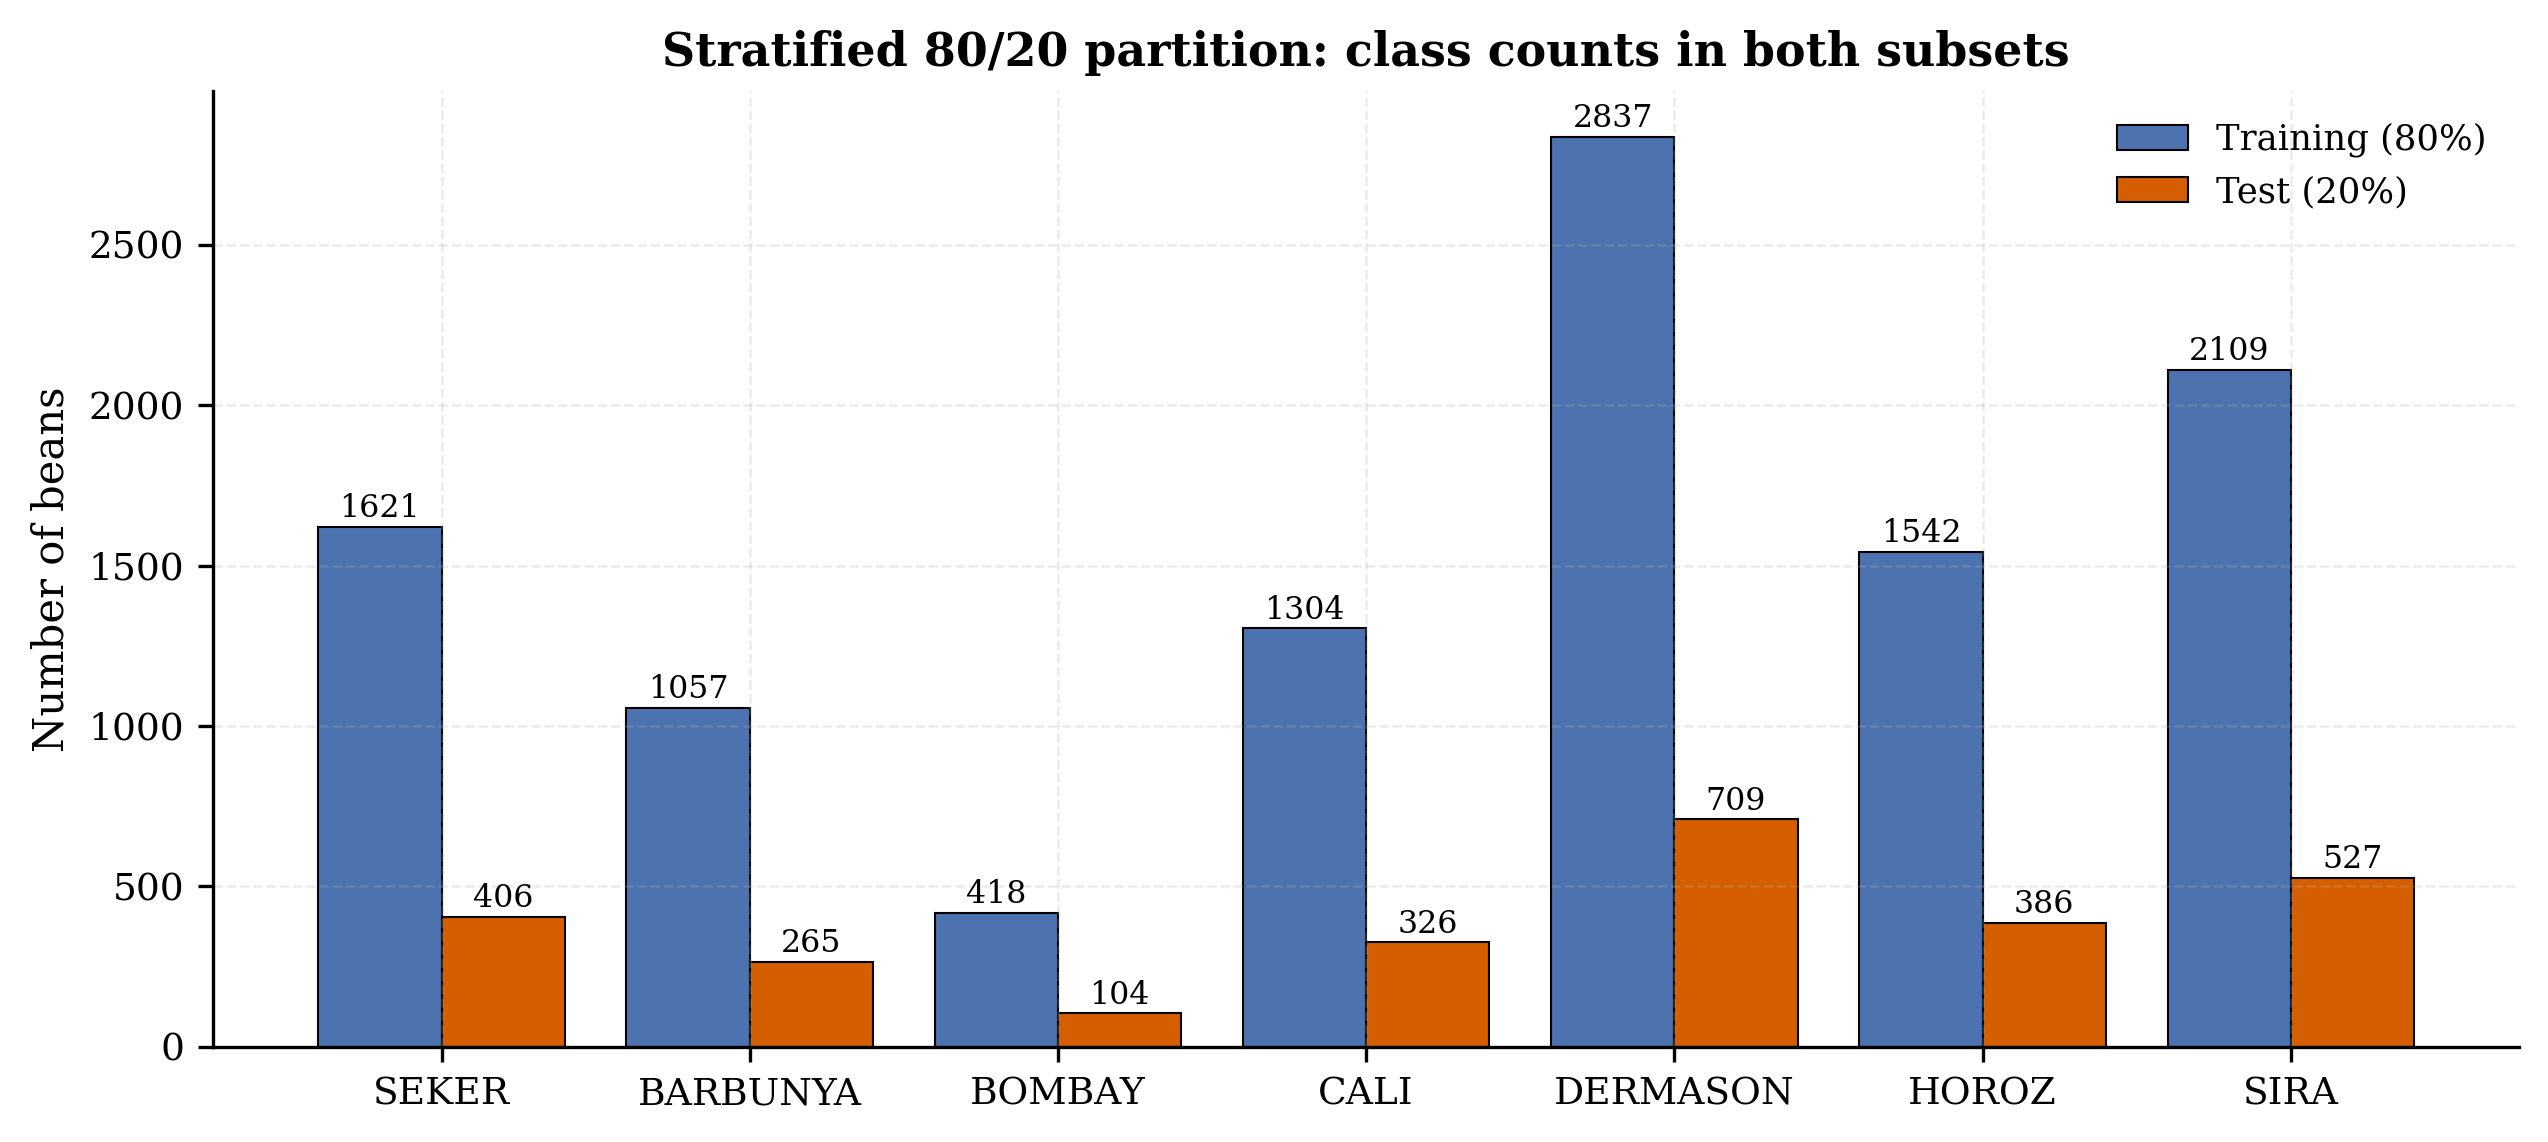
\includegraphics[width=0.80\textwidth]{fig_4_1_split.png}
\caption{Stratified partition of the dataset. The class proportions are preserved
to within 0.1 percentage points in both subsets.}
\label{fig:splitbar}
\end{figure}

The training partition supplies both model fitting and model selection: the
hyperparameter search uses stratified five-fold cross-validation inside the
\TrainRows{} training beans, so each candidate configuration is scored on five
disjoint validation folds of roughly 2,178 beans. The test partition of
\TestRows{} beans is evaluated once, in Chapter~6, after the model has been
chosen. No test observation influences the choice of algorithm, the search space
or any hyperparameter value.

Four leakage controls were enforced and are checked by the test suite:

\begin{enumerate}[label=(\alph*)]
  \item the split is written to \texttt{data/processed/} and every later stage
        reads those files, so the partition cannot drift between experiments;
  \item the scaler is fitted inside the pipeline, on training folds only;
  \item no oversampling, undersampling or class weighting is applied before the
        split; class weighting is evaluated as a controlled experiment inside
        cross-validation (Table~\ref{tab:class_weight});
  \item the feature ablation in Section~4.3 uses cross-validation on the training
        partition only, so the comparison cannot be biased by test data.
\end{enumerate}

The class-imbalance experiment deserves a note. The literature reviewed in
Chapter~2 suggests resampling the minority classes \cite{lee2024}. Rather than
adopt that recommendation, the effect of balanced class weights was measured on
the training partition with the same folds used for model selection. The result,
in Table~\ref{tab:class_weight}, is that balanced weights lower the
cross-validated macro F1 of the selected model from \CWNone{} to \CWBalanced{}.
The original class distribution was therefore kept throughout. The reason is
visible in Figure~\ref{fig:class_distribution}: with 522 Bombay beans and a
feature that separates them almost perfectly, the minority class is not being
suppressed by the majority; reweighting only distorts the decision boundary
elsewhere.

\begin{table}[htbp]
\centering
\small
\caption{Effect of balanced class weights on the selected model}
\label{tab:class_weight}
\begin{tabular}{llrr}
\toprule
Model & class\_weight & CV macro F1 & Std. dev. \\
\midrule
RBF-SVM & none & 0.9420 & 0.0052 \\
RBF-SVM & balanced & 0.9407 & 0.0052 \\
\bottomrule
\end{tabular}
\end{table}


\chapter{MACHINE LEARNING MODEL DEVELOPMENT}

\section{Workflow and System Architecture}

Figure~\ref{fig:workflow} shows the pipeline that produced every number in this
report. It is implemented as importable modules under \texttt{src/} rather than as
a single notebook, so that the notebooks, the tests and the report generator all
call the same code. The three columns correspond to the three partitions of the
data: preparation, learning and assessment. The horizontal connectors mark the
only points at which data moves between them, which is what makes the leakage
argument in Section~4.4 checkable: the test partition is not reachable from the
learning column.

\begin{figure}[htbp]
\centering
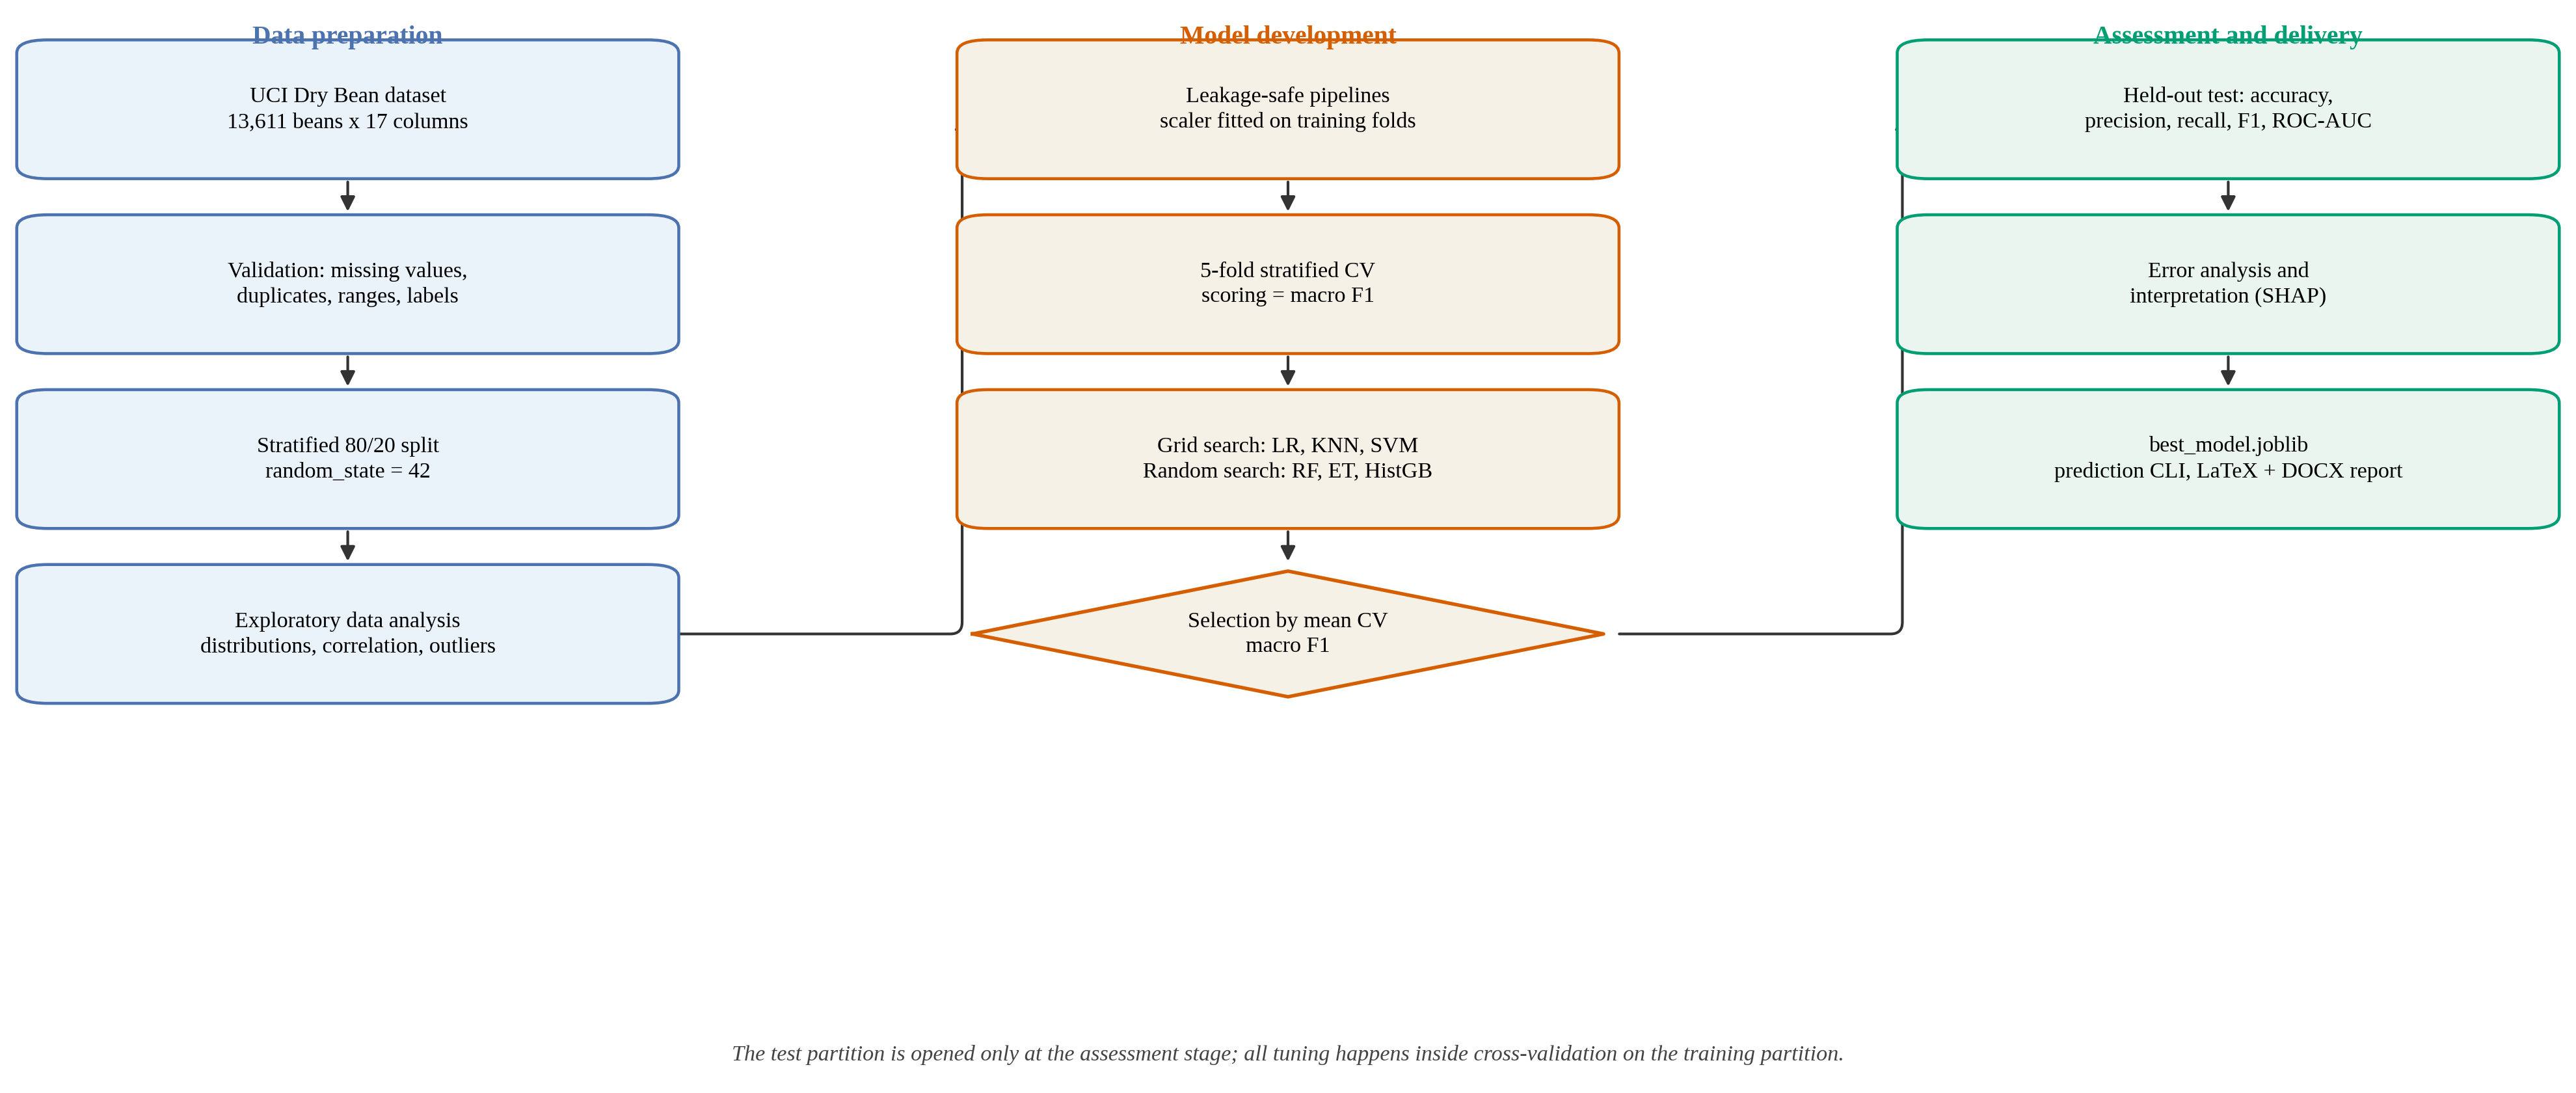
\includegraphics[width=\textwidth]{fig_5_1_workflow.png}
\caption{End-to-end workflow. Model selection happens entirely inside the training
partition; the test partition is opened once, at the assessment stage.}
\label{fig:workflow}
\end{figure}

\section{Algorithms Selected}

Six classifiers were chosen so that the comparison spans the four classical
inductive biases: a linear decision boundary, a local instance-based rule, a
maximum-margin boundary in a kernel-induced space, and randomised tree ensembles.
The sixth, histogram gradient boosting, is included because the case-study brief
allows it and because it represents the boosted-tree family that the reviewed
literature does not cover on this dataset.

\subsection{Logistic Regression}

Multinomial logistic regression models the posterior of class $k$ as
\begin{equation}
  P(y = k \mid \mathbf{x}) =
  \frac{\exp(\mathbf{w}_k^{\top}\mathbf{x} + b_k)}
       {\sum_{j=1}^{K}\exp(\mathbf{w}_j^{\top}\mathbf{x} + b_j)},
  \qquad k = 1,\dots,K,
  \label{eq:softmax}
\end{equation}
and is fitted by minimising the L2-regularised negative log-likelihood
\begin{equation}
  J(\mathbf{W}, \mathbf{b}) =
  -\frac{1}{N}\sum_{i=1}^{N}\log P(y_i \mid \mathbf{x}_i)
  + \frac{1}{2C}\sum_{k=1}^{K}\|\mathbf{w}_k\|_2^{2}.
  \label{eq:lr-objective}
\end{equation}
The parameter $C$ is the inverse regularisation strength: small $C$ shrinks the
coefficients towards zero, large $C$ allows them to grow and lets the model fit
the training data more closely. The model has $K(d+1) = 7 \times 17 = 119$
parameters, solved here with the L-BFGS quasi-Newton method.

Logistic regression is included as the linear baseline, not as a candidate for the
final model. Its decision boundaries are hyperplanes in the 16-dimensional input
space, so it can only separate classes that are linearly separable or nearly so.
The exploratory analysis in Chapter~3 already indicates that this is false for the
five overlapping varieties: Cali and Barbunya differ mainly in a ratio, and a
hyperplane through standardised coordinates cannot express that cleanly. The
baseline quantifies how much accuracy the nonlinear models actually add.

\subsection{k-Nearest Neighbours}

kNN assigns the majority label among the $k$ nearest training points,
\begin{equation}
  \hat{y}(\mathbf{x}) =
  \arg\max_{c}\ \sum_{i \in \mathcal{N}_k(\mathbf{x})} w_i\,
  \mathbf{1}[y_i = c],
  \label{eq:knn}
\end{equation}
where $\mathcal{N}_k(\mathbf{x})$ is the set of $k$ nearest neighbours under a
chosen metric and $w_i = 1$ for uniform voting or $w_i = 1/d(\mathbf{x},
\mathbf{x}_i)$ for distance weighting. Euclidean and Manhattan metrics are both
searched, with $k \in \{1,3,5,\dots,41\}$.

The method has no training phase and no parametric assumption, which makes it a
useful contrast: it can represent arbitrarily curved boundaries, but it does so
purely from local density. Two properties make it sensitive here. It is entirely
dependent on the metric, so unscaled features would reduce it to a nearest-
\texttt{Area} rule; standardisation is therefore mandatory. And in 16 dimensions
the ratio between the nearest and farthest neighbour distances shrinks, so
distances become less discriminative as the feature set grows, which is the
curse of dimensionality. With 10,888 training beans and seven classes the
prediction cost is also non-trivial, since every query compares against the whole
training set.

\subsection{Support Vector Machine with an RBF Kernel}

The SVM finds the maximum-margin separating hyperplane \cite{cortes1995}. In its soft-margin primal
form for a binary problem,
\begin{equation}
  \min_{\mathbf{w}, b, \boldsymbol{\xi}}\ \
  \frac{1}{2}\|\mathbf{w}\|^{2} + C\sum_{i=1}^{N}\xi_i
  \quad\text{subject to}\quad
  y_i\big(\mathbf{w}^{\top}\phi(\mathbf{x}_i) + b\big) \ge 1 - \xi_i,\ \
  \xi_i \ge 0,
  \label{eq:svm-primal}
\end{equation}
where $\phi$ maps the inputs into a higher-dimensional space, $\xi_i$ are slack
variables that permit margin violations and $C$ prices those violations. The dual
form depends on the data only through inner products, so replacing
$\phi(\mathbf{x}_i)^{\top}\phi(\mathbf{x}_j)$ by a kernel $K(\mathbf{x}_i,
\mathbf{x}_j)$ gives a nonlinear classifier without ever computing $\phi$
explicitly. The radial basis function kernel used here is
\begin{equation}
  K(\mathbf{x}, \mathbf{x}') =
  \exp\!\big(-\gamma\|\mathbf{x} - \mathbf{x}'\|^{2}\big),
  \label{eq:rbf}
\end{equation}
whose single parameter $\gamma$ sets the width of the influence of a training
point. The decision function is
$\hat{y}(\mathbf{x}) = \operatorname{sign}\big(\sum_i \alpha_i y_i
K(\mathbf{x}_i, \mathbf{x}) + b\big)$, and only the points with $\alpha_i > 0$,
the support vectors, contribute.

The two hyperparameters have opposite and interacting effects. Large $C$ penalises
margin violations heavily, producing a wiggly boundary that follows the training
data; small $C$ produces a smoother boundary that may underfit. Large $\gamma$
makes each training point influential only in a small neighbourhood, which again
overfits; small $\gamma$ makes the kernel almost linear. Because the effects
interact, both were searched jointly over a $4\times4$ grid rather than tuned one
at a time. The SVM is the primary candidate for this dataset because the class
boundaries are expected to be curved but not arbitrarily so: the EDA shows
compact, roughly ellipsoidal clusters, which is the geometry an RBF kernel
represents well.

One implementation detail matters for the results. The binary formulation above
does not extend directly to seven classes. scikit-learn's \texttt{SVC} uses the
one-versus-one scheme, training $\binom{7}{2} = 21$ binary classifiers and
deciding by a voting scheme, so the fitted model contains 21 margins rather than
one. The reported predictions are therefore the output of a pairwise voting
procedure, not of a single seven-way optimisation. Class probabilities, where
needed for the ROC curves, are obtained by Platt scaling \cite{platt1999}, which
fits a logistic model to the decision values using an internal cross-validation.

\subsection{Random Forest}

A random forest \cite{breiman2001} averages $T$ decision trees, each grown on a bootstrap sample of
the training data and, at every split, allowed to consider only a random subset of
$\lfloor\sqrt{d}\rfloor$ or $\lfloor 0.5d\rfloor$ features. Splits are chosen to
maximise the decrease in Gini impurity
\begin{equation}
  G(t) = 1 - \sum_{k=1}^{K} p_{k\mid t}^{2},
  \label{eq:gini}
\end{equation}
where $p_{k\mid t}$ is the proportion of class $k$ in node $t$. The prediction is
the majority vote of the $T$ trees.

The two sources of randomness decorrelate the trees, and averaging correlated
predictors with variance $\sigma^2$ and pairwise correlation $\rho$ gives an
ensemble variance of roughly
\begin{equation}
  \operatorname{Var}\!\left(\frac{1}{T}\sum_{t=1}^{T} h_t(\mathbf{x})\right)
  = \rho\sigma^{2} + \frac{1-\rho}{T}\sigma^{2},
  \label{eq:rf-variance}
\end{equation}
so the benefit comes from lowering $\rho$, not from adding trees indefinitely.
That is why the number of trees is a cost parameter rather than a tuning
parameter: increasing $T$ reduces the second term only, and the first term is
controlled by the feature subsampling. For this reason $T$ was fixed at 300 and
only the structural parameters were searched.

Random forests are included because they make no assumption about the shape of the
boundary, are invariant to monotone rescaling, and handle the redundant features
of Chapter~3 without difficulty: if two columns carry the same information, the
forest simply uses whichever is drawn at a given node. Their weakness is that
axis-aligned splits approximate diagonal or ratio-based boundaries only with many
small steps, which is exactly the geometry that separates Cali from Barbunya.

\subsection{Extra Trees}

Extremely randomised trees \cite{geurts2006} use the same ensemble structure but differ in one
respect: instead of searching for the best threshold at each node, a random
threshold is drawn for each candidate feature and the best of those random splits
is kept. The trees are therefore more strongly randomised and individually more
biased, but less correlated, which by Equation~\ref{eq:rf-variance} can reduce
ensemble variance. The method also trains faster, because no sorting of candidate
thresholds is required. The comparison between Random Forest and Extra Trees is
therefore a direct test of whether the extra randomisation helps on this feature
set, with everything else held constant.

\subsection{Histogram Gradient Boosting}

Gradient boosting fits trees sequentially, each one to the negative gradient of
the loss with respect to the current ensemble prediction. The histogram variant
discretises each feature into at most 255 bins, which makes split search
$O(N)$ per feature and allows deep ensembles to be trained quickly. The learning
rate, number of boosting rounds, leaf count, minimum leaf size and L2 penalty were
searched. Boosting is included as a sixth model because it often outperforms
bagging on tabular data with moderate sample size, and because including it makes
the comparison cover both ensemble strategies.

\section{Implementation Details}

The implementation is Python 3.12.13 with NumPy 2.3.4 \cite{harris2020},
pandas 2.3.3 \cite{mckinney2010}, scikit-learn 1.7.2 \cite{pedregosa2011},
SciPy 1.16.2 \cite{virtanen2020}, Matplotlib 3.10.7 \cite{hunter2007} and
seaborn 0.13.2 \cite{waskom2021}. All
experiments ran on a 12-core x86-64 desktop with 30~GB of RAM and no GPU; the
pipeline never uses one. The complete run, from download to the last SHAP plot,
takes \PipelineMinutes{} minutes.

Table~\ref{tab:modules} lists the modules and their responsibilities. Each module
is importable, has a \texttt{\_\_main\_\_} entry point where that makes sense, and
writes its outputs to a fixed directory, so any stage can be re-run alone.

\begin{table}[htbp]
\centering
\caption{Implementation modules}
\label{tab:modules}
\small
\begin{tabularx}{\textwidth}{@{}lX@{}}
\toprule
\textbf{Module} & \textbf{Responsibility} \\
\midrule
\texttt{config.py} & paths, random seed, feature order, colour palette, plot style \\
\texttt{data\_loader.py} & download, load, integrity validation, JSON report \\
\texttt{preprocessing.py} & stratified split, pipeline factory, split artefacts \\
\texttt{eda.py} & descriptive statistics and all Chapter 3 figures \\
\texttt{train.py} & model zoo, grid and random search, selection, ablations \\
\texttt{evaluate.py} & held-out metrics, confusion matrices, ROC, error analysis \\
\texttt{explainability.py} & impurity, permutation and SHAP importance \\
\texttt{predict.py} & command-line and programmatic prediction \\
\texttt{run\_pipeline.py} & orchestration of the six stages \\
\bottomrule
\end{tabularx}
\end{table}

Two implementation decisions affect the runtime and are worth recording. First,
parallelism is applied at the level of the cross-validation search: each candidate
configuration is evaluated in a separate process, which is the only effective
option for the SVM because the underlying libsvm solver is single-threaded. Nested
parallelism was deliberately avoided, since running a multi-threaded forest inside
a multi-process search oversubscribes the cores and makes the run slower.
Second, the search spaces were pruned of configurations that cannot change the
model. With 16 features, \texttt{max\_features="sqrt"}, \texttt{"log2"} and
\texttt{0.3} all select four features and are therefore the same estimator; only
\texttt{"sqrt"} and \texttt{0.5} are retained. Similarly,
\texttt{n\_estimators} is fixed rather than searched. Removing those redundant
candidates cut the Random Forest search from 296~s to 184~s without changing the
selected model.

The prediction interface is a single function, shown in
Listing~\ref{lst:predict}, wrapped by a command-line entry point that accepts
either a CSV of measurements or all 16 values as flags.

\begin{lstlisting}[style=pycode, caption={Programmatic prediction. The saved
pipeline carries its own scaler, so callers never see raw feature scaling.},
label={lst:predict}]
def predict_records(records, model=None):
    model = model or load_model()
    frame = pd.DataFrame(records)[FEATURES].astype(float)
    proba = probabilities(model, frame)
    classes = list(model.classes_)
    ranked = np.argsort(proba[0])[::-1]
    return classes[ranked[0]], proba[0][ranked[0]]
\end{lstlisting}

\section{Hyperparameter Settings}

Table~\ref{tab:search_space} records the search space of every model. Grid search
was used where the space is small and its structure is interpretable (logistic
regression, kNN, SVM); randomised search with 25 and 20 draws was used for the
ensembles, where the product of the individual grids would be in the thousands and
most of that volume is uninformative. Every search used the same stratified
five-fold splitter with a fixed seed, so candidate configurations within a model
are compared on identical folds.

\begin{table}[htbp]
\centering
\caption{Hyperparameter search spaces}
\label{tab:search_space}
\footnotesize
\begin{tabularx}{\textwidth}{@{}p{2.5cm}p{4.6cm}p{4.2cm}X@{}}
\toprule
\textbf{Model} & \textbf{Hyperparameter} & \textbf{Values} & \textbf{Method} \\
\midrule
Logistic Regression & \texttt{C} & 0.01, 0.1, 1, 10, 100 & Grid (5) \\
\addlinespace
KNN & \texttt{n\_neighbors} & 1, 3, 5, 7, 9, 11, 15, 21, 31, 41 & \multirow{3}{*}{Grid (40)} \\
 & \texttt{weights} & uniform, distance & \\
 & \texttt{metric} & euclidean, manhattan & \\
\addlinespace
RBF-SVM & \texttt{C} & 0.1, 1, 10, 100 & \multirow{2}{*}{Grid (16)} \\
 & \texttt{gamma} & scale, 0.001, 0.01, 0.1 & \\
\addlinespace
Random Forest & \texttt{max\_depth} & None, 20, 30, 40 & \multirow{5}{*}{Random (25)} \\
 & \texttt{min\_samples\_split} & 2, 5, 10 & \\
 & \texttt{min\_samples\_leaf} & 1, 2, 4 & \\
 & \texttt{max\_features} & sqrt, 0.5 & \\
 & \texttt{n\_estimators} & fixed at 300 & \\
\addlinespace
Extra Trees & \texttt{max\_depth} & None, 20, 30, 40 & \multirow{5}{*}{Random (25)} \\
 & \texttt{min\_samples\_split} & 2, 5, 10 & \\
 & \texttt{min\_samples\_leaf} & 1, 2, 4 & \\
 & \texttt{max\_features} & sqrt, 0.5 & \\
 & \texttt{n\_estimators} & fixed at 300 & \\
\addlinespace
Hist Gradient Boosting & \texttt{learning\_rate} & 0.05, 0.1, 0.2 & \multirow{5}{*}{Random (20)} \\
 & \texttt{max\_iter} & 200, 400, 600 & \\
 & \texttt{max\_leaf\_nodes} & 31, 63 & \\
 & \texttt{min\_samples\_leaf} & 20, 50 & \\
 & \texttt{l2\_regularization} & 0.0, 1.0 & \\
\bottomrule
\end{tabularx}
\end{table}

Table~\ref{tab:best_params} lists the configuration selected for each model.
Figure~\ref{fig:svmgrid} shows the full SVM surface. It is flat between $C = 1$
and $C = 100$ at $\gamma = 0.01$, which means that once the margin penalty is
large enough the additional capacity is unused: the classes are already almost
separable in the induced space. The two failure modes appear at the corners.
$C = 0.1$ with $\gamma = 0.001$ underfits, because the kernel is too wide and the
penalty too weak to place a boundary; $\gamma = 0.1$ degrades every value of $C$,
because each training point then influences only its immediate neighbourhood and
the margin fragments.

\begin{table}[htbp]
\centering
\footnotesize
\caption{Best configuration of every model, chosen by mean 5-fold CV macro F1}
\label{tab:best_params}
\begin{tabular}{p{0.26\textwidth}p{0.64\textwidth}}
\toprule
Model & Selected hyperparameters \\
\midrule
RBF-SVM & C = 100.0, gamma = 0.01 \\
Hist Gradient Boosting & min\_samples\_leaf = 20, max\_leaf\_nodes = 63, max\_iter = 400, learning\_rate = 0.1, l2\_regularization = 1.0 \\
K-Nearest Neighbours & metric = euclidean, n\_neighbors = 9, weights = distance \\
Random Forest & min\_samples\_split = 10, min\_samples\_leaf = 2, max\_features = 0.5, max\_depth = 30 \\
Logistic Regression & C = 100.0 \\
Extra Trees & min\_samples\_split = 10, min\_samples\_leaf = 2, max\_features = 0.5, max\_depth = 30 \\
\bottomrule
\end{tabular}
\end{table}


\begin{figure}[htbp]
\centering
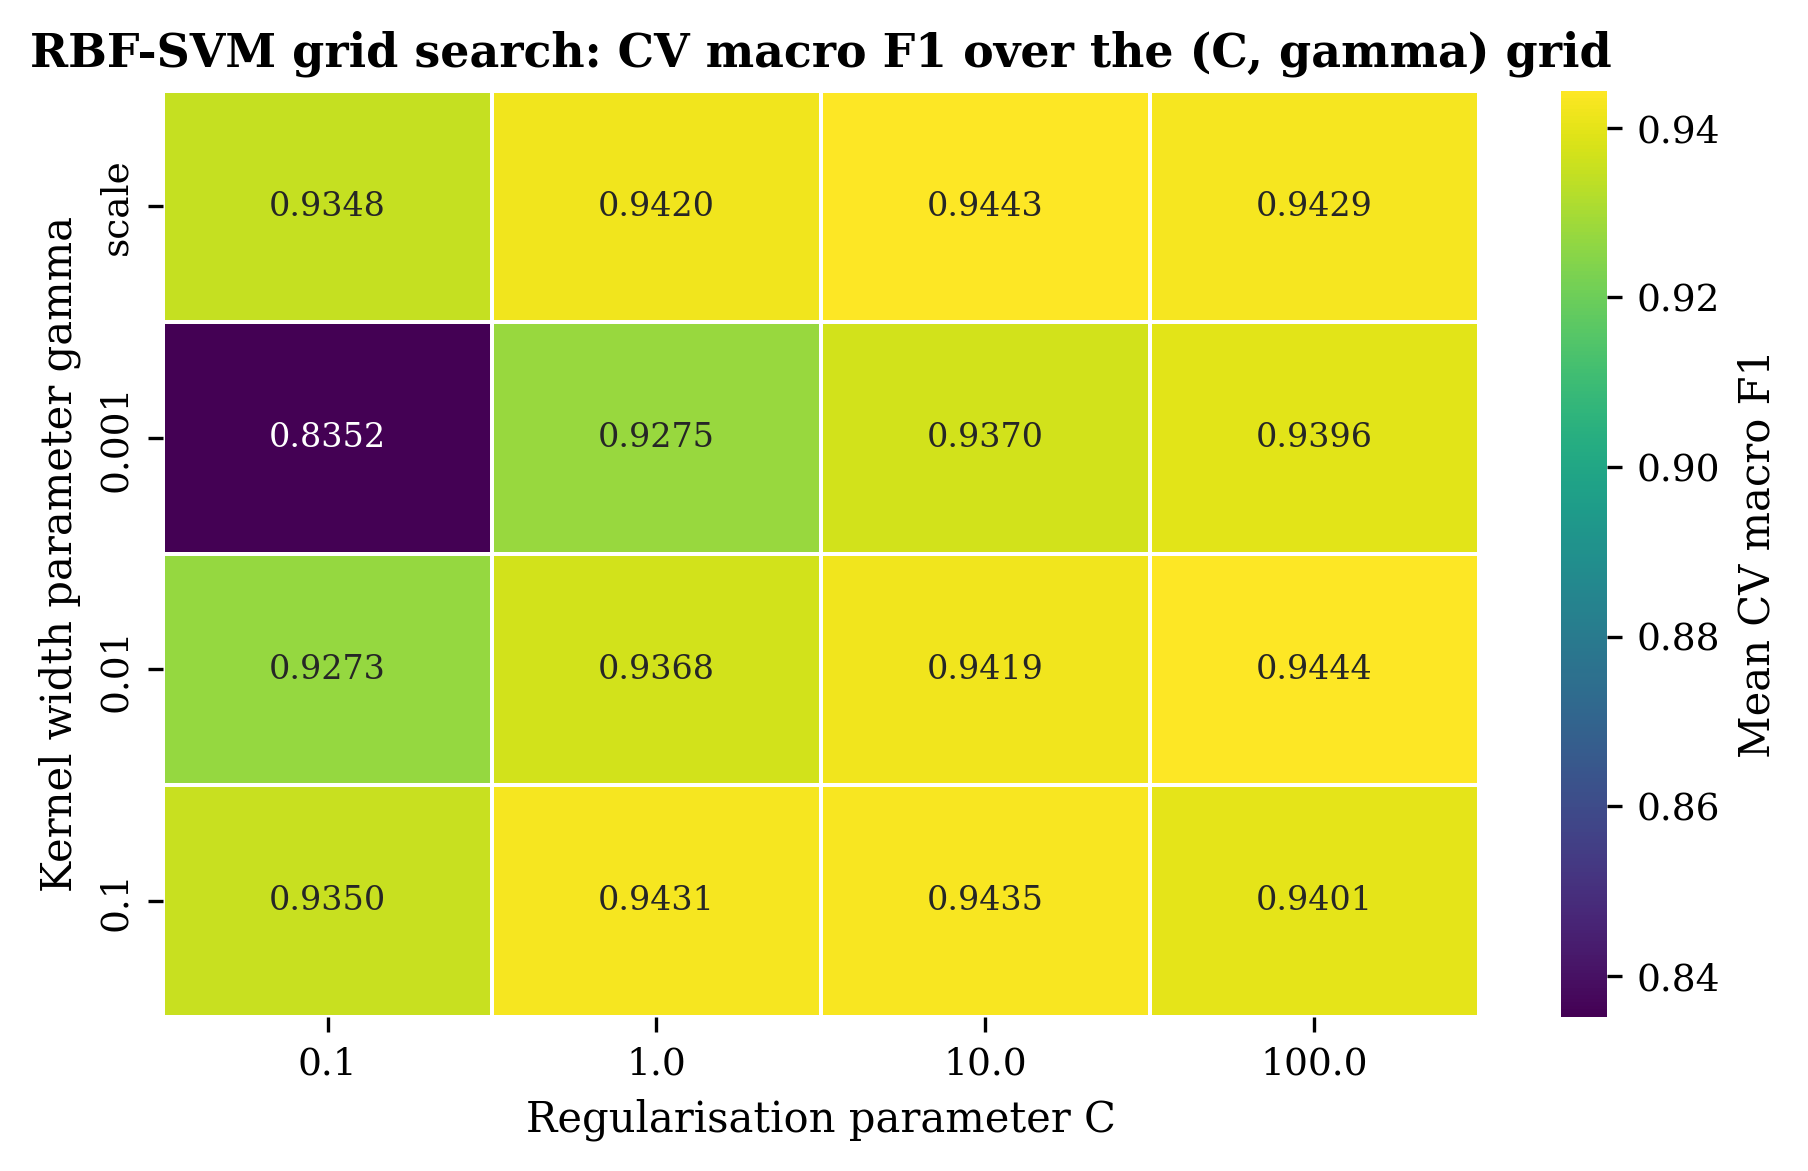
\includegraphics[width=0.60\textwidth]{fig_5_2_svm_grid_search.png}
\caption{Cross-validated macro F1 over the RBF-SVM $(\gamma, C)$ grid. The surface
is flat along the $C$ axis for $\gamma = 0.01$ and collapses at $\gamma = 0.1$.}
\label{fig:svmgrid}
\end{figure}

\chapter{RESULTS AND PERFORMANCE EVALUATION}

\section{Evaluation Metrics}

For a seven-class problem, let $TP_c$, $FP_c$ and $FN_c$ be the true positives,
false positives and false negatives of class $c$. Per-class precision, recall and
F1 are
\begin{equation}
  P_c = \frac{TP_c}{TP_c + FP_c}, \qquad
  R_c = \frac{TP_c}{TP_c + FN_c}, \qquad
  F1_c = \frac{2P_cR_c}{P_c + R_c},
  \label{eq:prf}
\end{equation}
and the two aggregations used in this report are
\begin{equation}
  \text{macro F1} = \frac{1}{K}\sum_{c=1}^{K} F1_c,
  \qquad
  \text{weighted F1} = \sum_{c=1}^{K}\frac{n_c}{N}\,F1_c ,
  \label{eq:aggregation}
\end{equation}
where $n_c$ is the number of test beans of class $c$. Accuracy is the trace of the
confusion matrix divided by $N$.

Macro F1 is the primary metric for two reasons. It weights every variety equally,
so a model cannot buy accuracy by sacrificing Bombay, which contributes only 3.84\%
of the beans; and it is a harmonic mean, so it punishes a model that achieves high
recall by predicting a class indiscriminately. Weighted F1 is reported alongside
it because it is the quantity a grading line actually experiences: it weights each
bean equally, so errors on the large classes count more. When the two diverge, the
difference localises the errors, and that is exactly what happens in
Table~\ref{tab:model_comparison}, where macro F1 exceeds accuracy for every model.

ROC-AUC is computed with the one-vs-rest strategy: for each variety, the
probability of that variety is treated as a score against all other varieties
combined, and the area under the resulting curve is averaged over the seven
classes. It measures ranking quality independently of the decision threshold,
which matters if the model is later given a rejection option.

\section{Experimental Results}

Table~\ref{tab:model_comparison} reports the held-out performance of all six
models, and Table~\ref{tab:cv_results} reports the cross-validated scores that
were used to select them. Figure~\ref{fig:comparison} shows the three main metrics
side by side.

\begin{table}[htbp]
\centering
\scriptsize
\caption{Performance on the 2,723-bean held-out test set. Rows are ordered by test macro F1}
\label{tab:model_comparison}
\begin{tabular}{lrrrrrr}
\toprule
Model & Accuracy & Macro prec. & Macro rec. & Macro F1 & Weighted F1 & ROC-AUC \\
\midrule
RBF-SVM & 0.9258 & 0.9383 & 0.9362 & 0.9372 & 0.9258 & 0.9953 \\
Hist Gradient Boosting & 0.9229 & 0.9368 & 0.9328 & 0.9347 & 0.9229 & 0.9948 \\
Logistic Regression & 0.9214 & 0.9357 & 0.9323 & 0.9337 & 0.9217 & 0.9949 \\
Extra Trees & 0.9207 & 0.9356 & 0.9306 & 0.9328 & 0.9208 & 0.9943 \\
Random Forest & 0.9196 & 0.9334 & 0.9297 & 0.9314 & 0.9195 & 0.9936 \\
K-Nearest Neighbours & 0.9174 & 0.9328 & 0.9279 & 0.9300 & 0.9175 & 0.9870 \\
\bottomrule
\end{tabular}
\end{table}


\begin{table}[htbp]
\centering
\footnotesize
\caption{Cross-validated macro F1 on the training partition (5 stratified folds). Sorted by mean macro F1}
\label{tab:cv_results}
\begin{tabular}{llcrrrrr}
\toprule
Model & Search & Configs & Mean & Std. dev. & Min & Max & Time (s) \\
\midrule
RBF-SVM & grid & 16 & 0.9444 & 0.0056 & 0.9391 & 0.9516 & 7.4 \\
Hist Gradient Boosting & random & 20 & 0.9424 & 0.0049 & 0.9379 & 0.9506 & 71.6 \\
K-Nearest Neighbours & grid & 40 & 0.9382 & 0.0048 & 0.9324 & 0.9426 & 4.1 \\
Random Forest & random & 25 & 0.9375 & 0.0037 & 0.9352 & 0.9440 & 183.9 \\
Logistic Regression & grid & 5 & 0.9374 & 0.0048 & 0.9321 & 0.9425 & 2.7 \\
Extra Trees & random & 25 & 0.9344 & 0.0033 & 0.9316 & 0.9402 & 24.4 \\
\bottomrule
\end{tabular}
\end{table}


\begin{figure}[htbp]
\centering
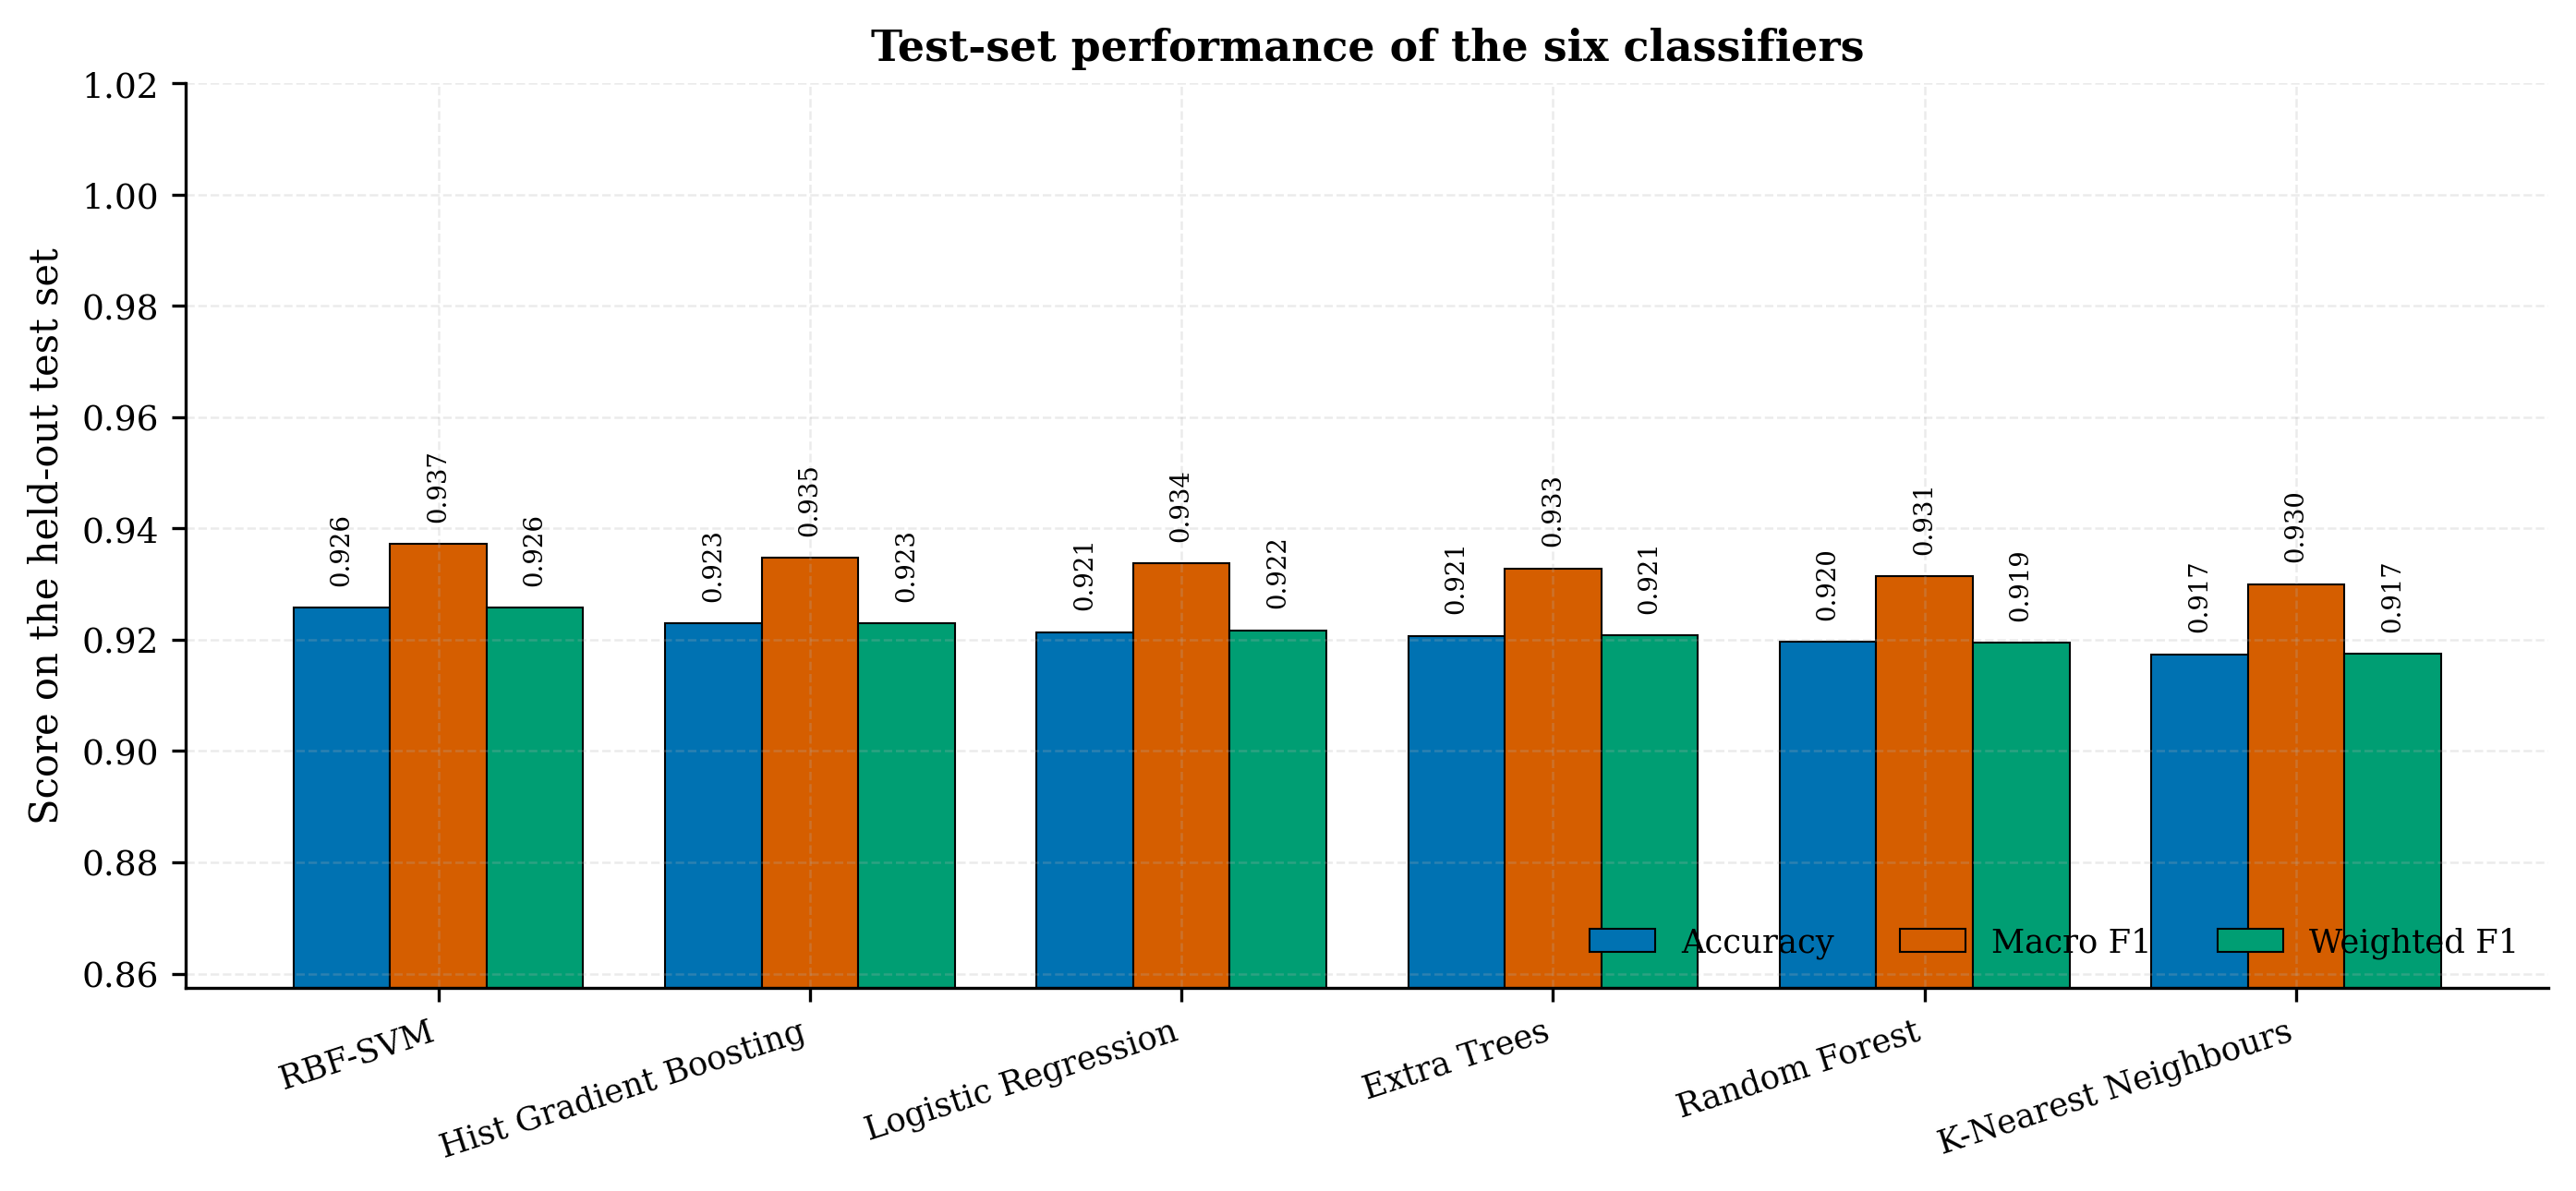
\includegraphics[width=0.82\textwidth]{fig_6_1_model_comparison.png}
\caption{Held-out accuracy, macro F1 and weighted F1 for the six classifiers. The
ordering is stable across the three metrics.}
\label{fig:comparison}
\end{figure}

The \BestModel{} leads on every metric: \BestAcc{} accuracy, \BestFOne{} macro F1,
\BestPrec{} macro precision, \BestRec{} macro recall and \BestAUC{} one-vs-rest
ROC-AUC. Histogram gradient boosting is second at \SecondFOne{} macro F1, and
k-nearest neighbours is last at \WorstFOne{}. The full spread from first to last
is 0.0072 macro F1, which corresponds to about 20 beans out of 2,723.

Two features of this table deserve comment before any interpretation.

First, macro F1 exceeds accuracy for all six models. This is not a paradox. The
two largest classes, Sira (527 test beans) and Dermason (709), carry most of the
errors, so they depress accuracy, which counts beans; Bombay, which is perfectly
classified, and Horoz and Seker, which are nearly so, raise the macro average,
which counts classes. A model with 0.9372 macro F1 and 0.9258 accuracy is
therefore a model that is excellent on five varieties and merely good on the two
largest ones.

Second, the cross-validated ranking in Table~\ref{tab:cv_results} is not the same
as the test ranking. k-nearest neighbours is third on cross-validation (0.9382) but
last on the test set (0.9300), while Extra Trees is last on cross-validation
(0.9344) but fourth on the test set (0.9328). The differences among the five
non-SVM models are between 0.002 and 0.004 macro F1, which is smaller than the
fold-to-fold standard deviation of 0.003 to 0.006 reported in the same table. The
honest reading is that those five models are statistically indistinguishable on
this dataset, and that their relative order on a single 2,723-bean test set is
partly noise. Only the SVM's advantage over the bottom of the table is larger than
the fold variance, and even that is modest.

\section{Visual Results}

Figure~\ref{fig:cmgrid} shows the six confusion matrices. The dominant feature is
common to all of them: the block formed by Sira and Dermason. In every model the
largest off-diagonal entries are Sira predicted as Dermason and Dermason predicted
as Sira. Bombay is classified perfectly by all six models, and Horoz and Seker are
almost always correct.

\begin{figure}[htbp]
\centering
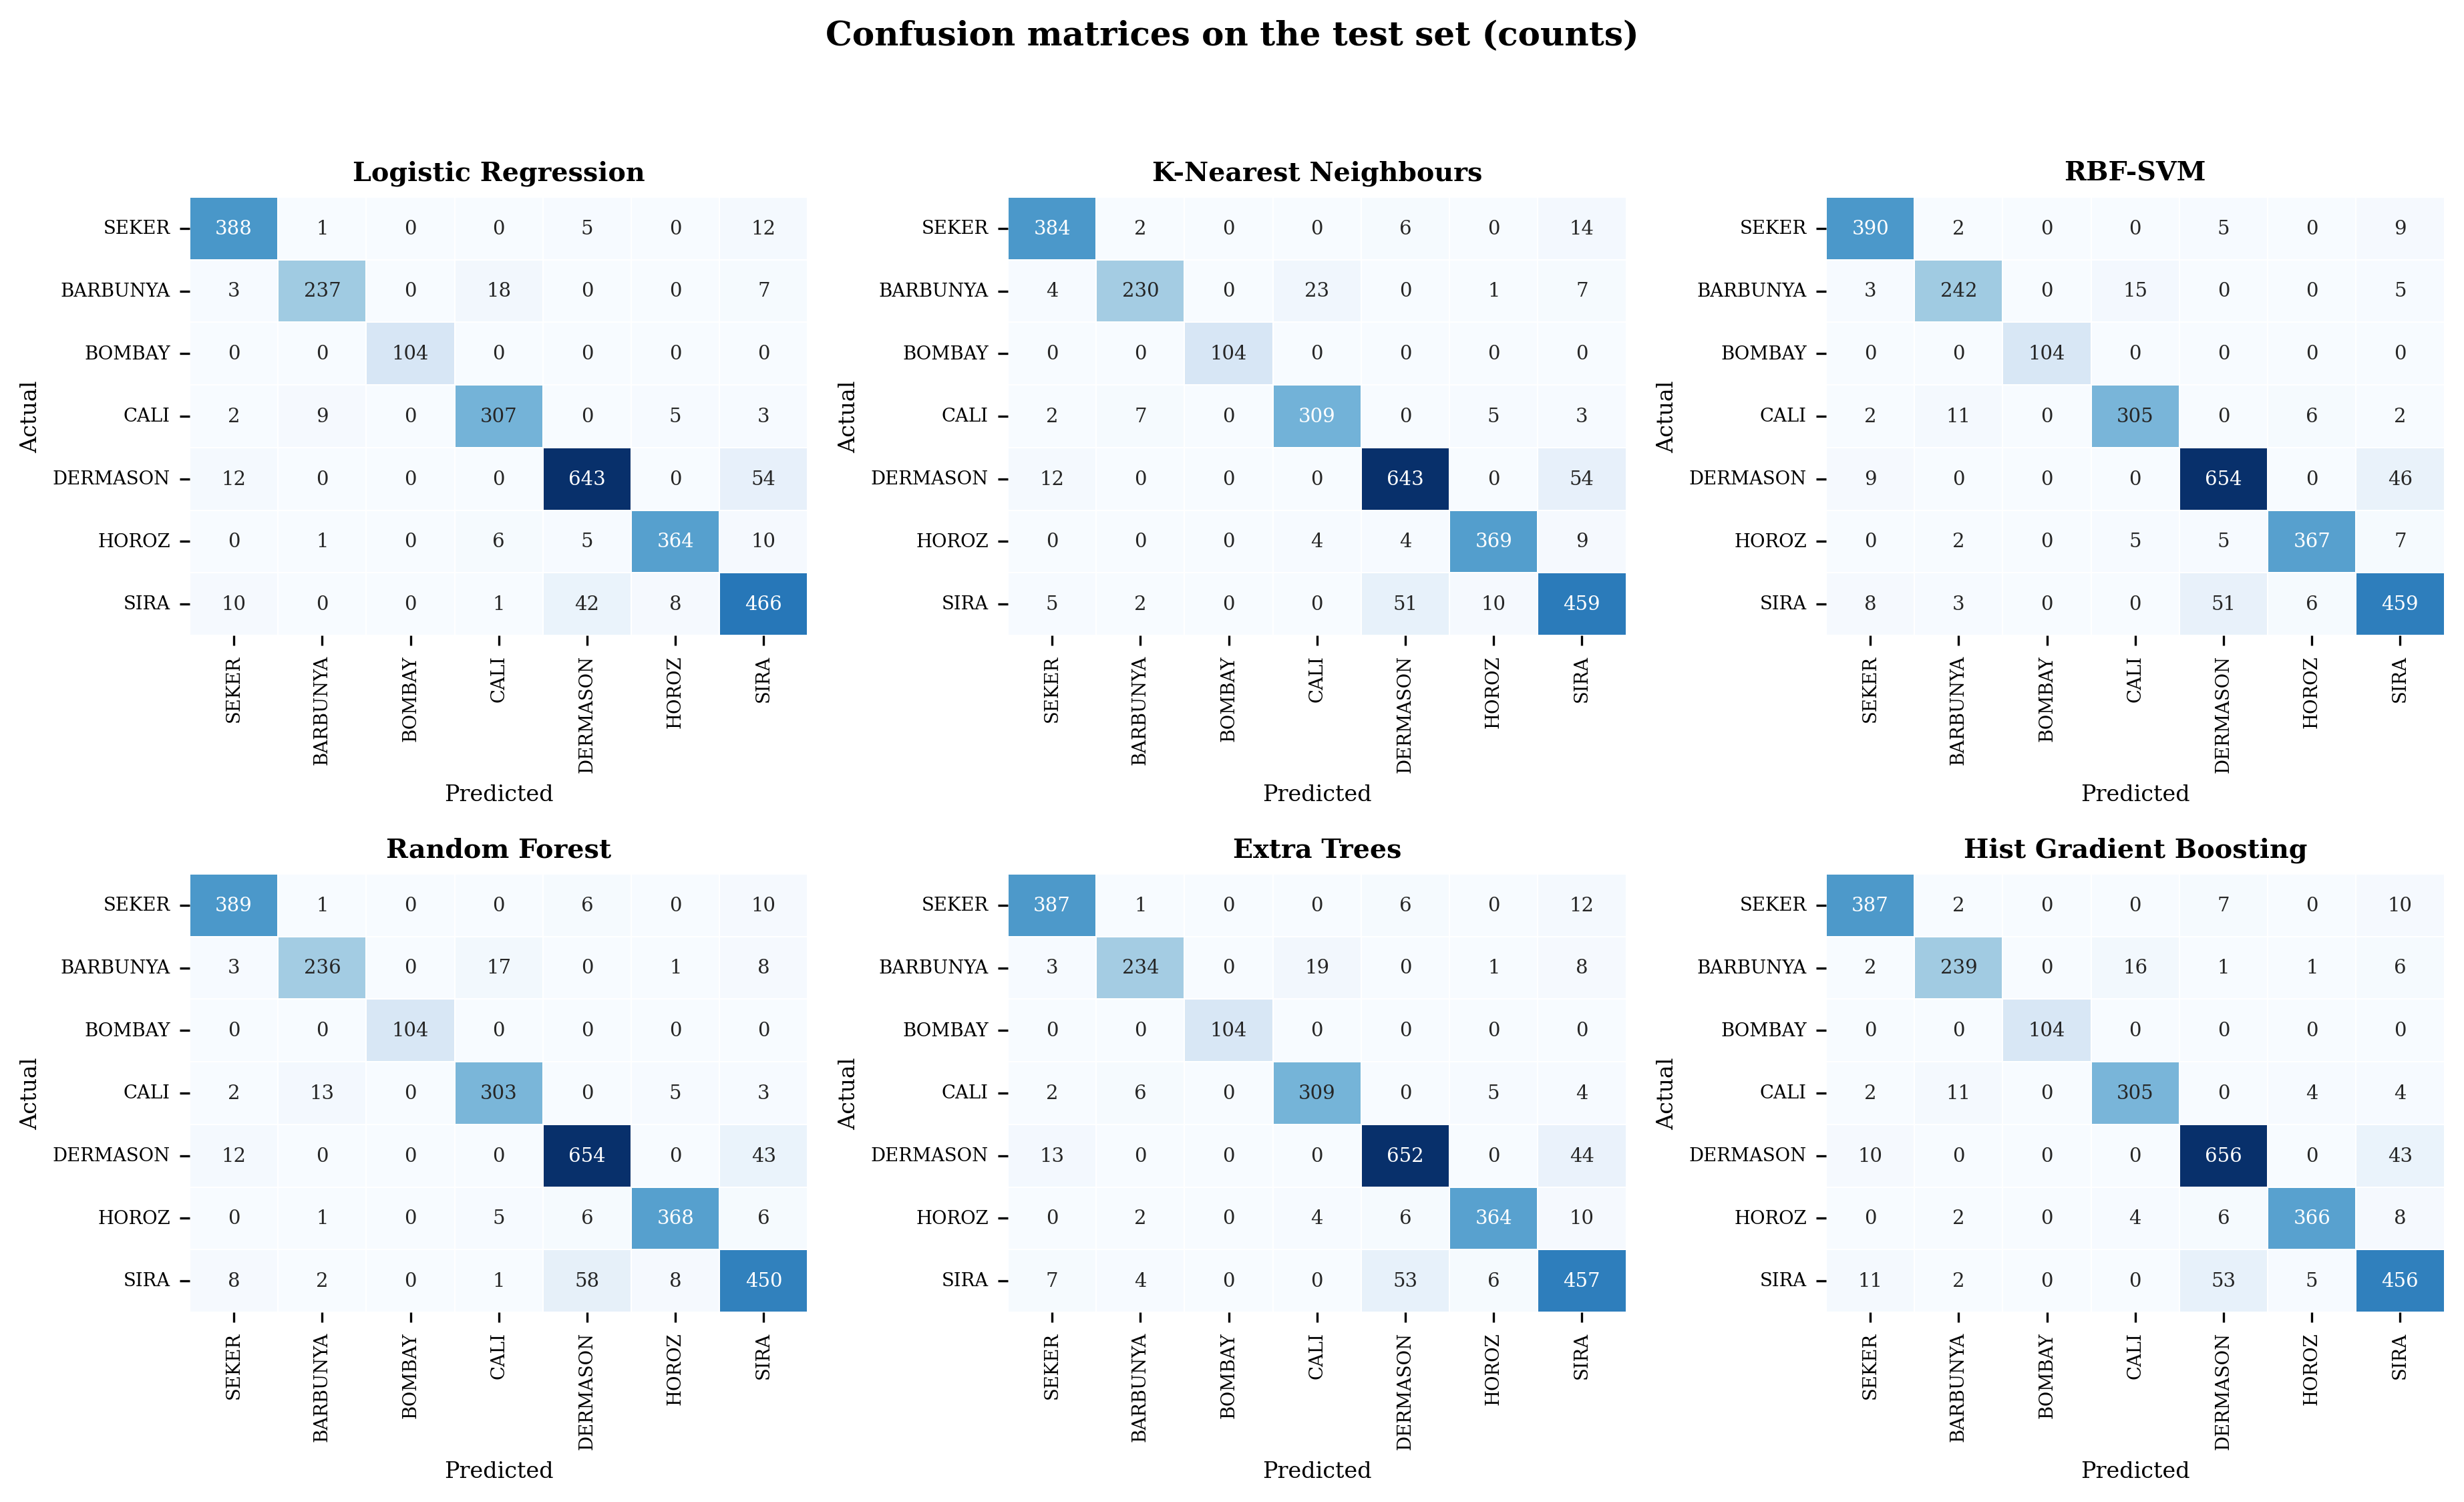
\includegraphics[width=0.94\textwidth]{fig_6_2_confusion_matrices.png}
\caption{Confusion matrices on the held-out test set. The Sira--Dermason block is
the dominant error source for every model.}
\label{fig:cmgrid}
\end{figure}

The row-normalised matrix of the selected model in Figure~\ref{fig:cmbest} makes
the magnitude explicit. Bombay, Horoz, Seker and Cali all exceed 0.93 on the
diagonal. Dermason and Sira are at 0.922 and 0.871, and the leakage between them
is 6.4\% of Dermason beans predicted as Sira and 9.7\% of Sira beans predicted as
Dermason.

\begin{figure}[htbp]
\centering
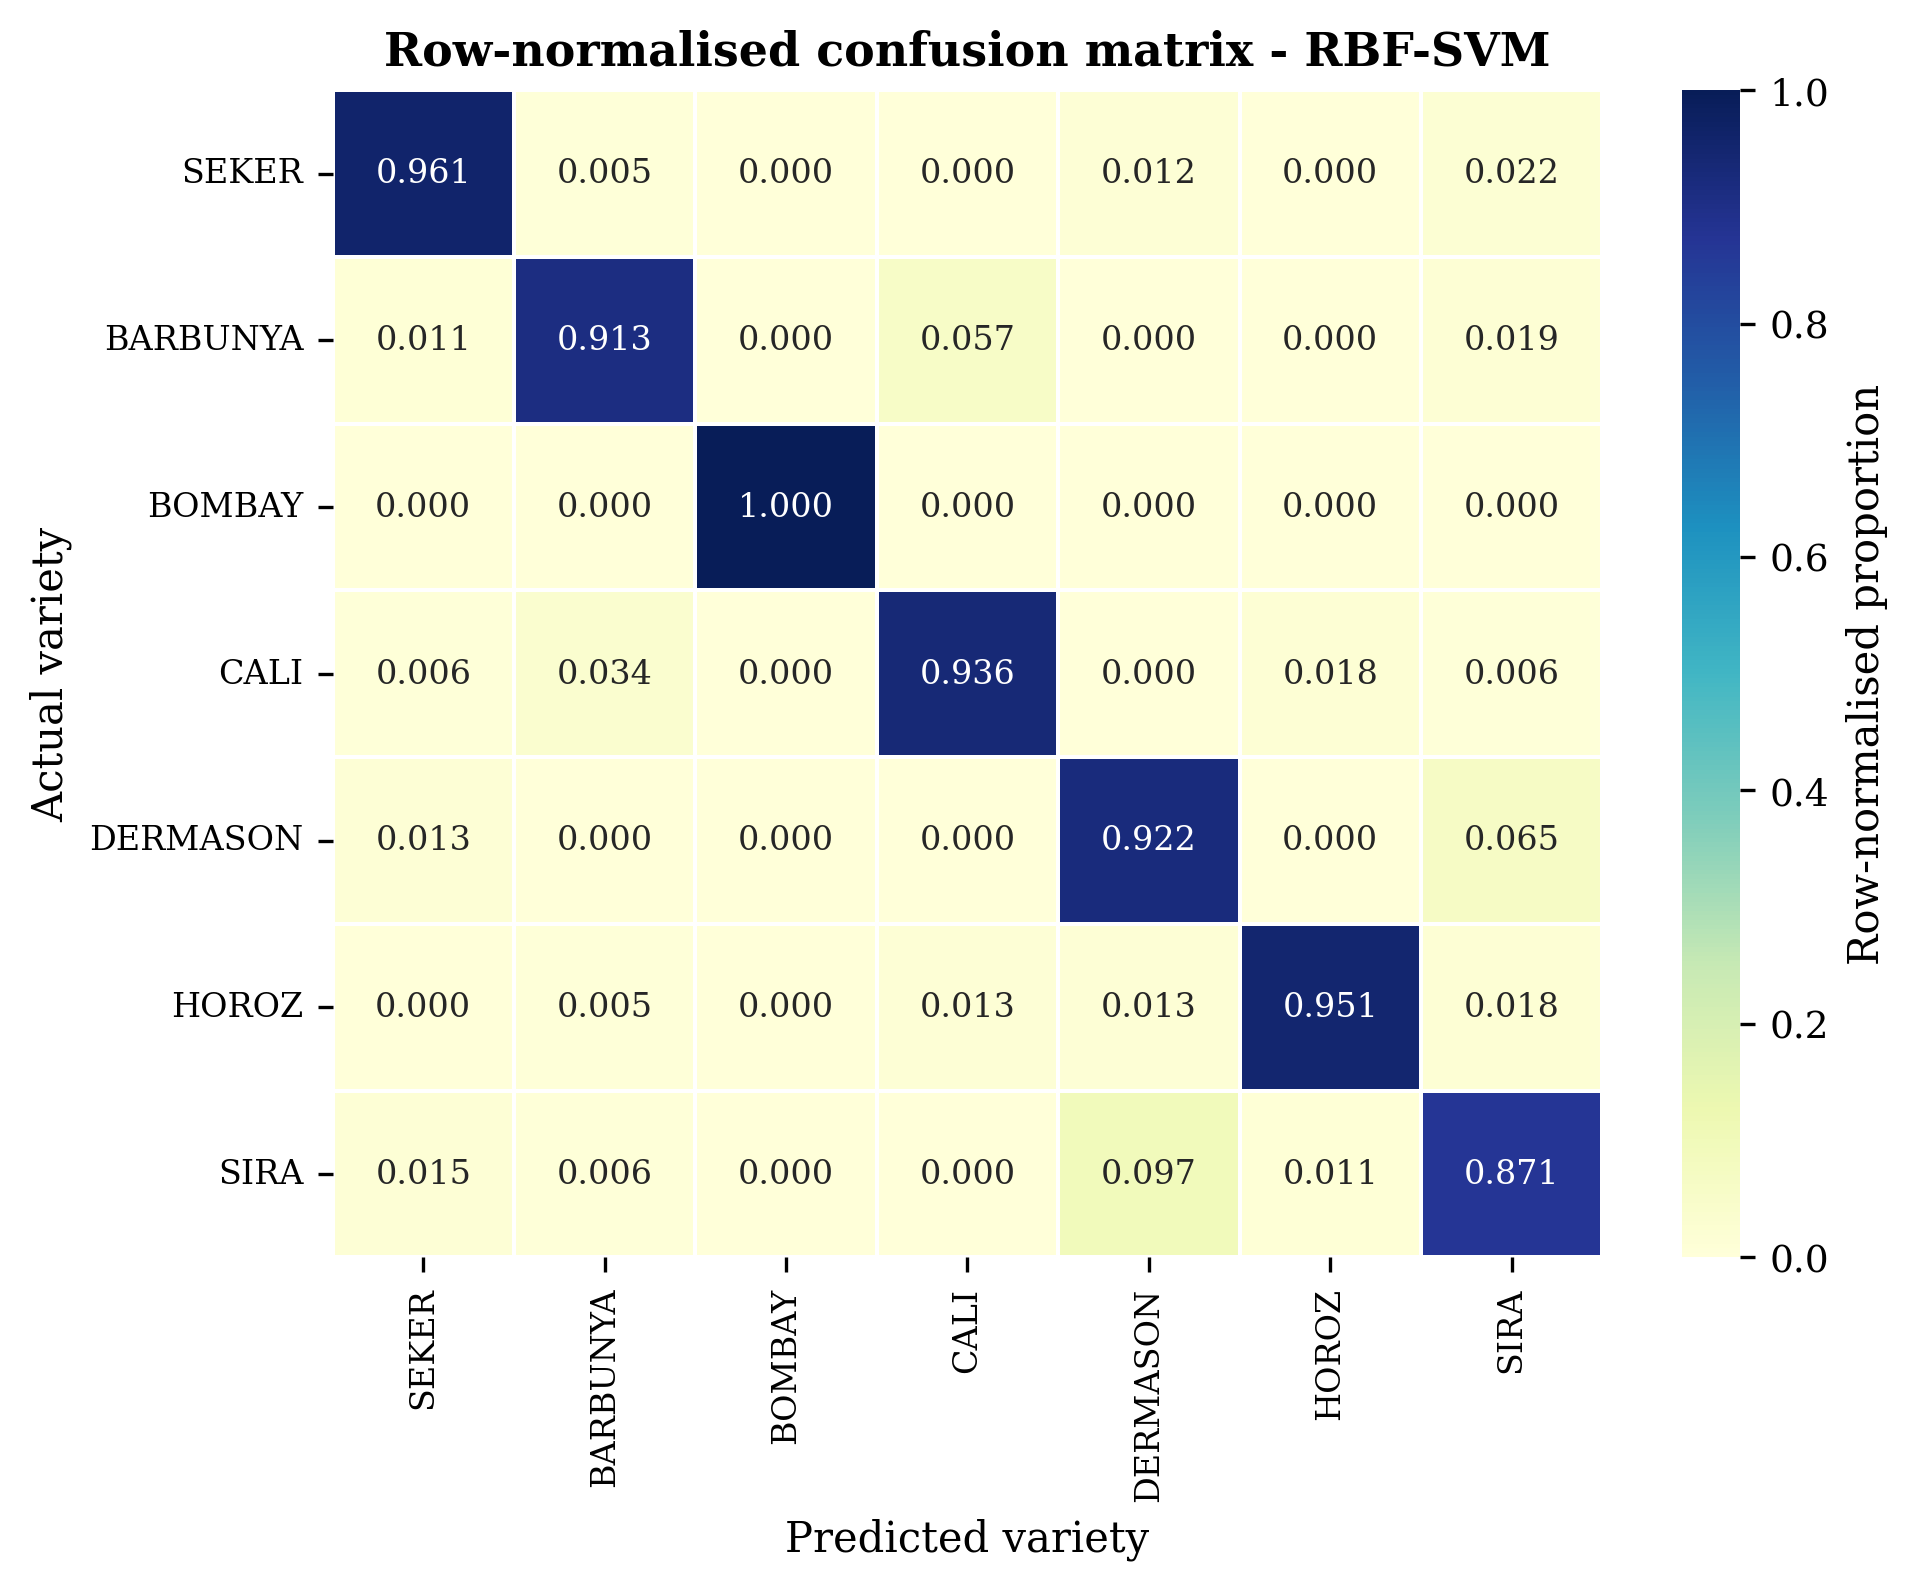
\includegraphics[width=0.58\textwidth]{fig_6_3_confusion_matrix_best.png}
\caption{Row-normalised confusion matrix of the \BestModel{}. Each row sums to
1.00; the diagonal is the per-class recall.}
\label{fig:cmbest}
\end{figure}

Table~\ref{tab:per_class} and Figure~\ref{fig:perclass} give the per-class scores.
Bombay reaches precision and recall of 1.000 on 104 test beans, which confirms the
expectation from Chapter~3 that its area separates it completely. Sira has the
lowest F1 at 0.8701, driven by a recall of 0.8710 rather than by poor precision
(0.8693), which means Sira beans are being absorbed by a neighbour rather than
being wrongly attracted into Sira. Horoz, which the EDA suggested might be
confusable, turns out to be the second-best class at 0.9595, because its extreme
compactness (0.701, the lowest of the seven) is a distinctive signal.

\begin{table}[htbp]
\centering
\small
\caption{Per-class performance of the selected model (RBF-SVM)}
\label{tab:per_class}
\begin{tabular}{lrrrr}
\toprule
Variety & Precision & Recall & F1-score & Support \\
\midrule
Seker & 0.9466 & 0.9606 & 0.9535 & 406 \\
Barbunya & 0.9308 & 0.9132 & 0.9219 & 265 \\
Bombay & 1.0000 & 1.0000 & 1.0000 & 104 \\
Cali & 0.9385 & 0.9356 & 0.9370 & 326 \\
Dermason & 0.9147 & 0.9224 & 0.9185 & 709 \\
Horoz & 0.9683 & 0.9508 & 0.9595 & 386 \\
Sira & 0.8693 & 0.8710 & 0.8701 & 527 \\
\midrule
Macro average & 0.9383 & 0.9362 & 0.9372 & 2723 \\
\bottomrule
\end{tabular}
\end{table}


\begin{figure}[htbp]
\centering
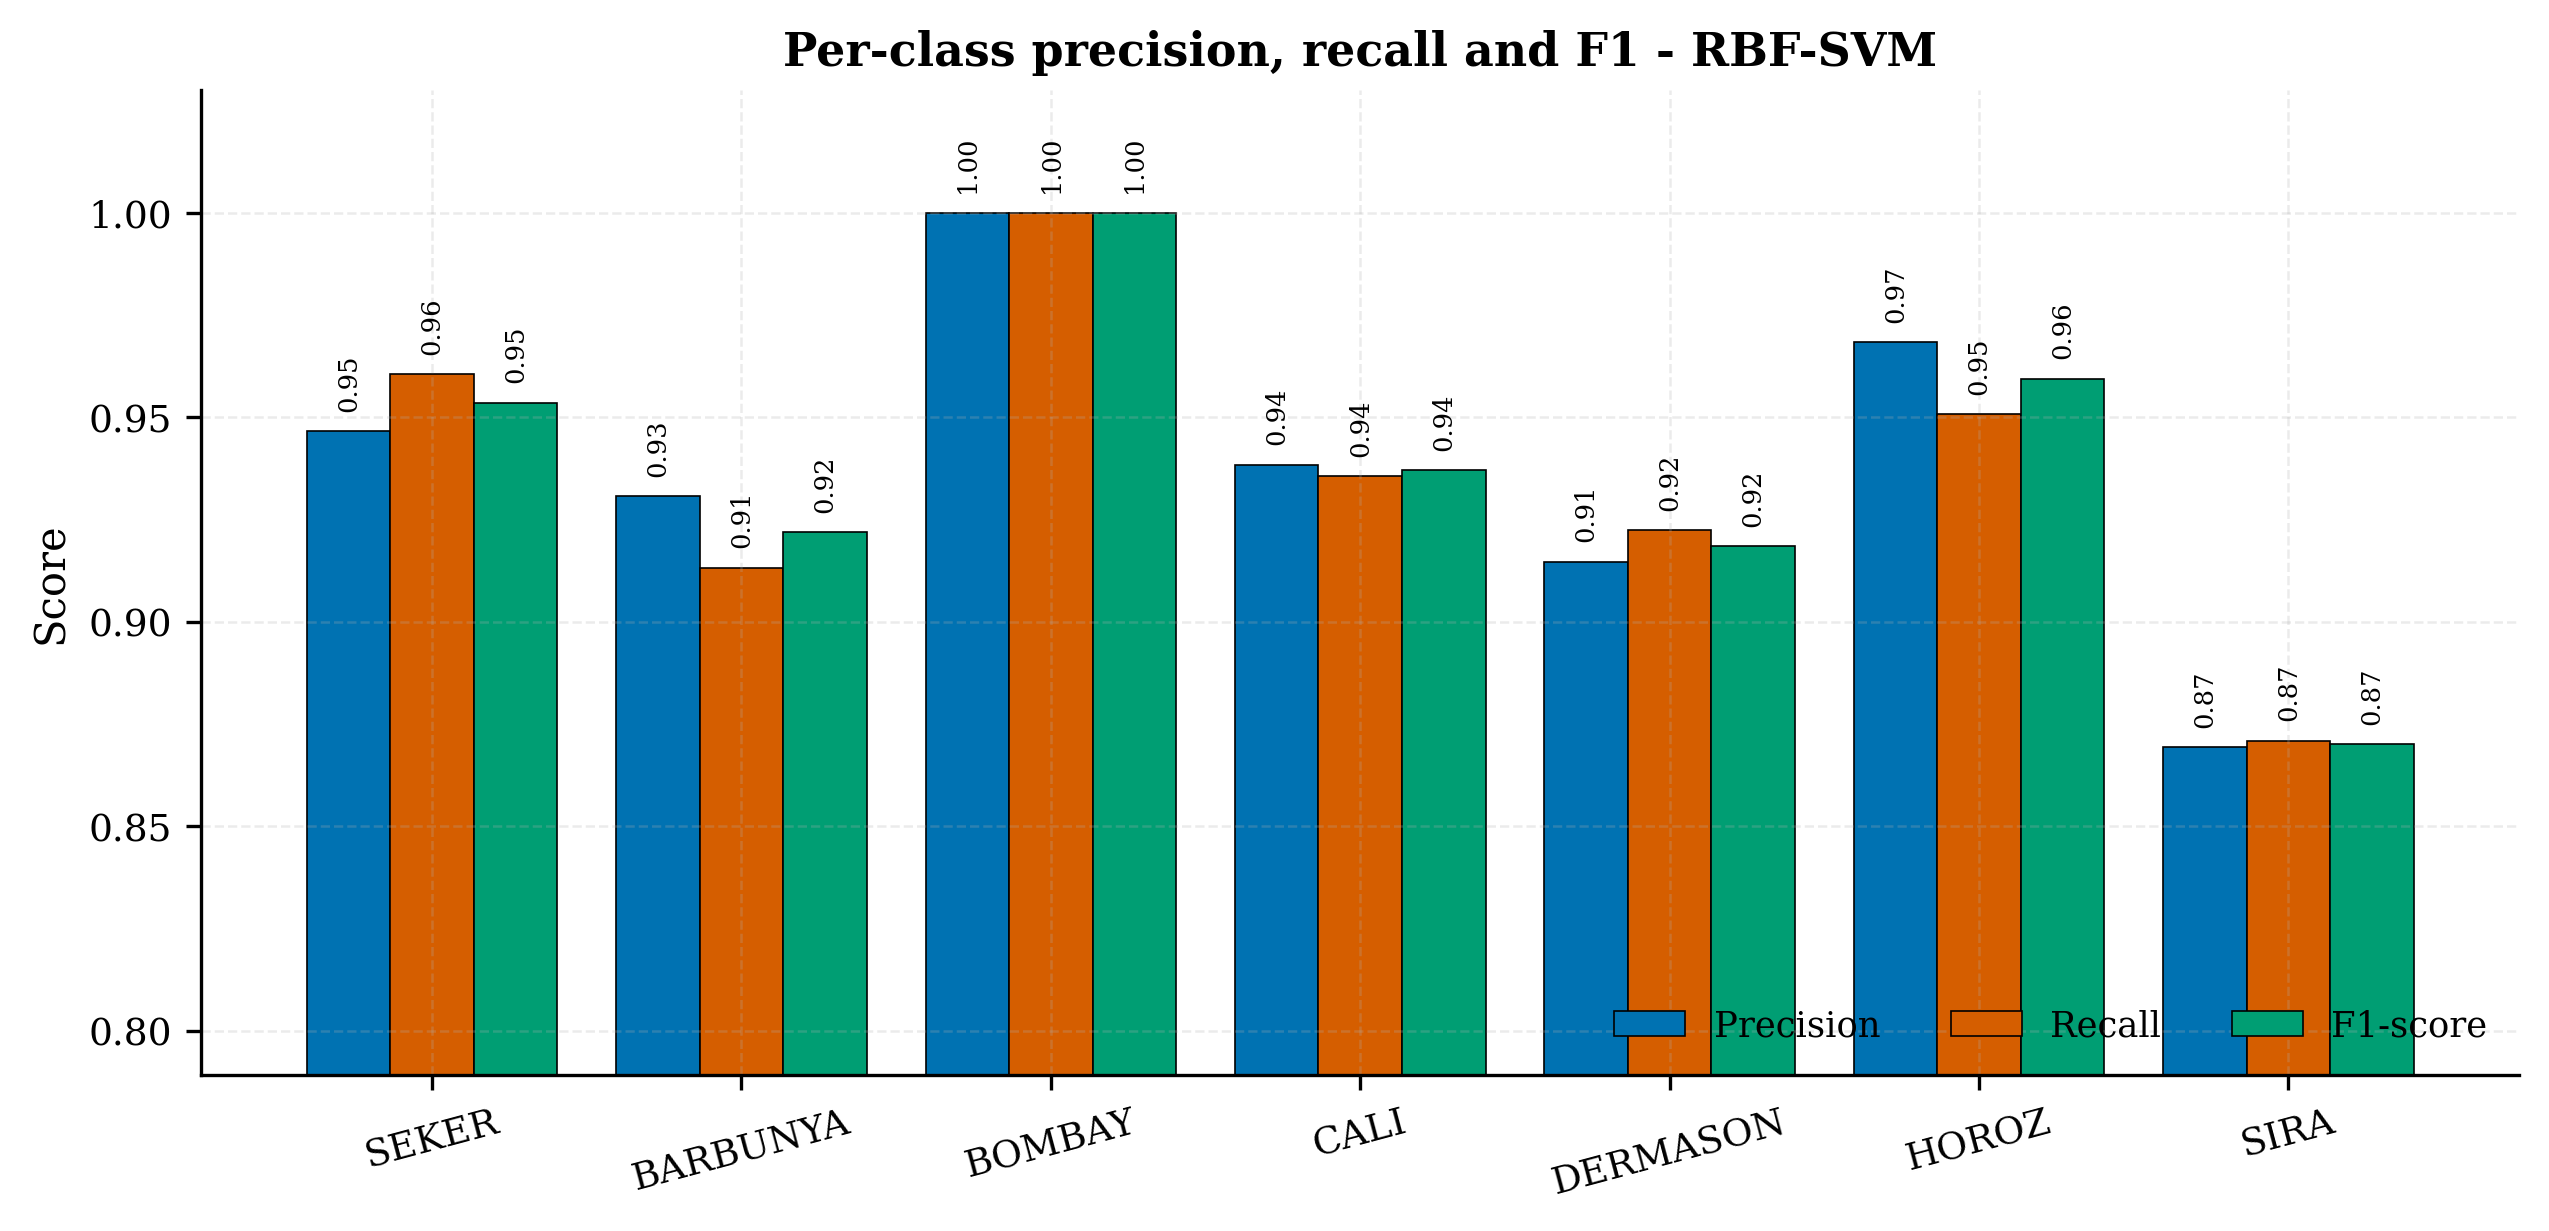
\includegraphics[width=0.78\textwidth]{fig_6_4_per_class_metrics.png}
\caption{Per-class precision, recall and F1 of the \BestModel{}. Bombay is
perfect; Sira is the weakest class.}
\label{fig:perclass}
\end{figure}

Figure~\ref{fig:roc} shows the one-vs-rest ROC curves. All seven areas exceed
0.986, and the macro average is \BestAUC. The curves confirm that the difficulty
is not in ranking beans by confidence but in the final decision at the boundary:
the model ranks a Sira bean above a Dermason bean 98.6\% of the time, yet still
misassigns 9.7\% of them once a single threshold is applied to all classes.

\begin{figure}[htbp]
\centering
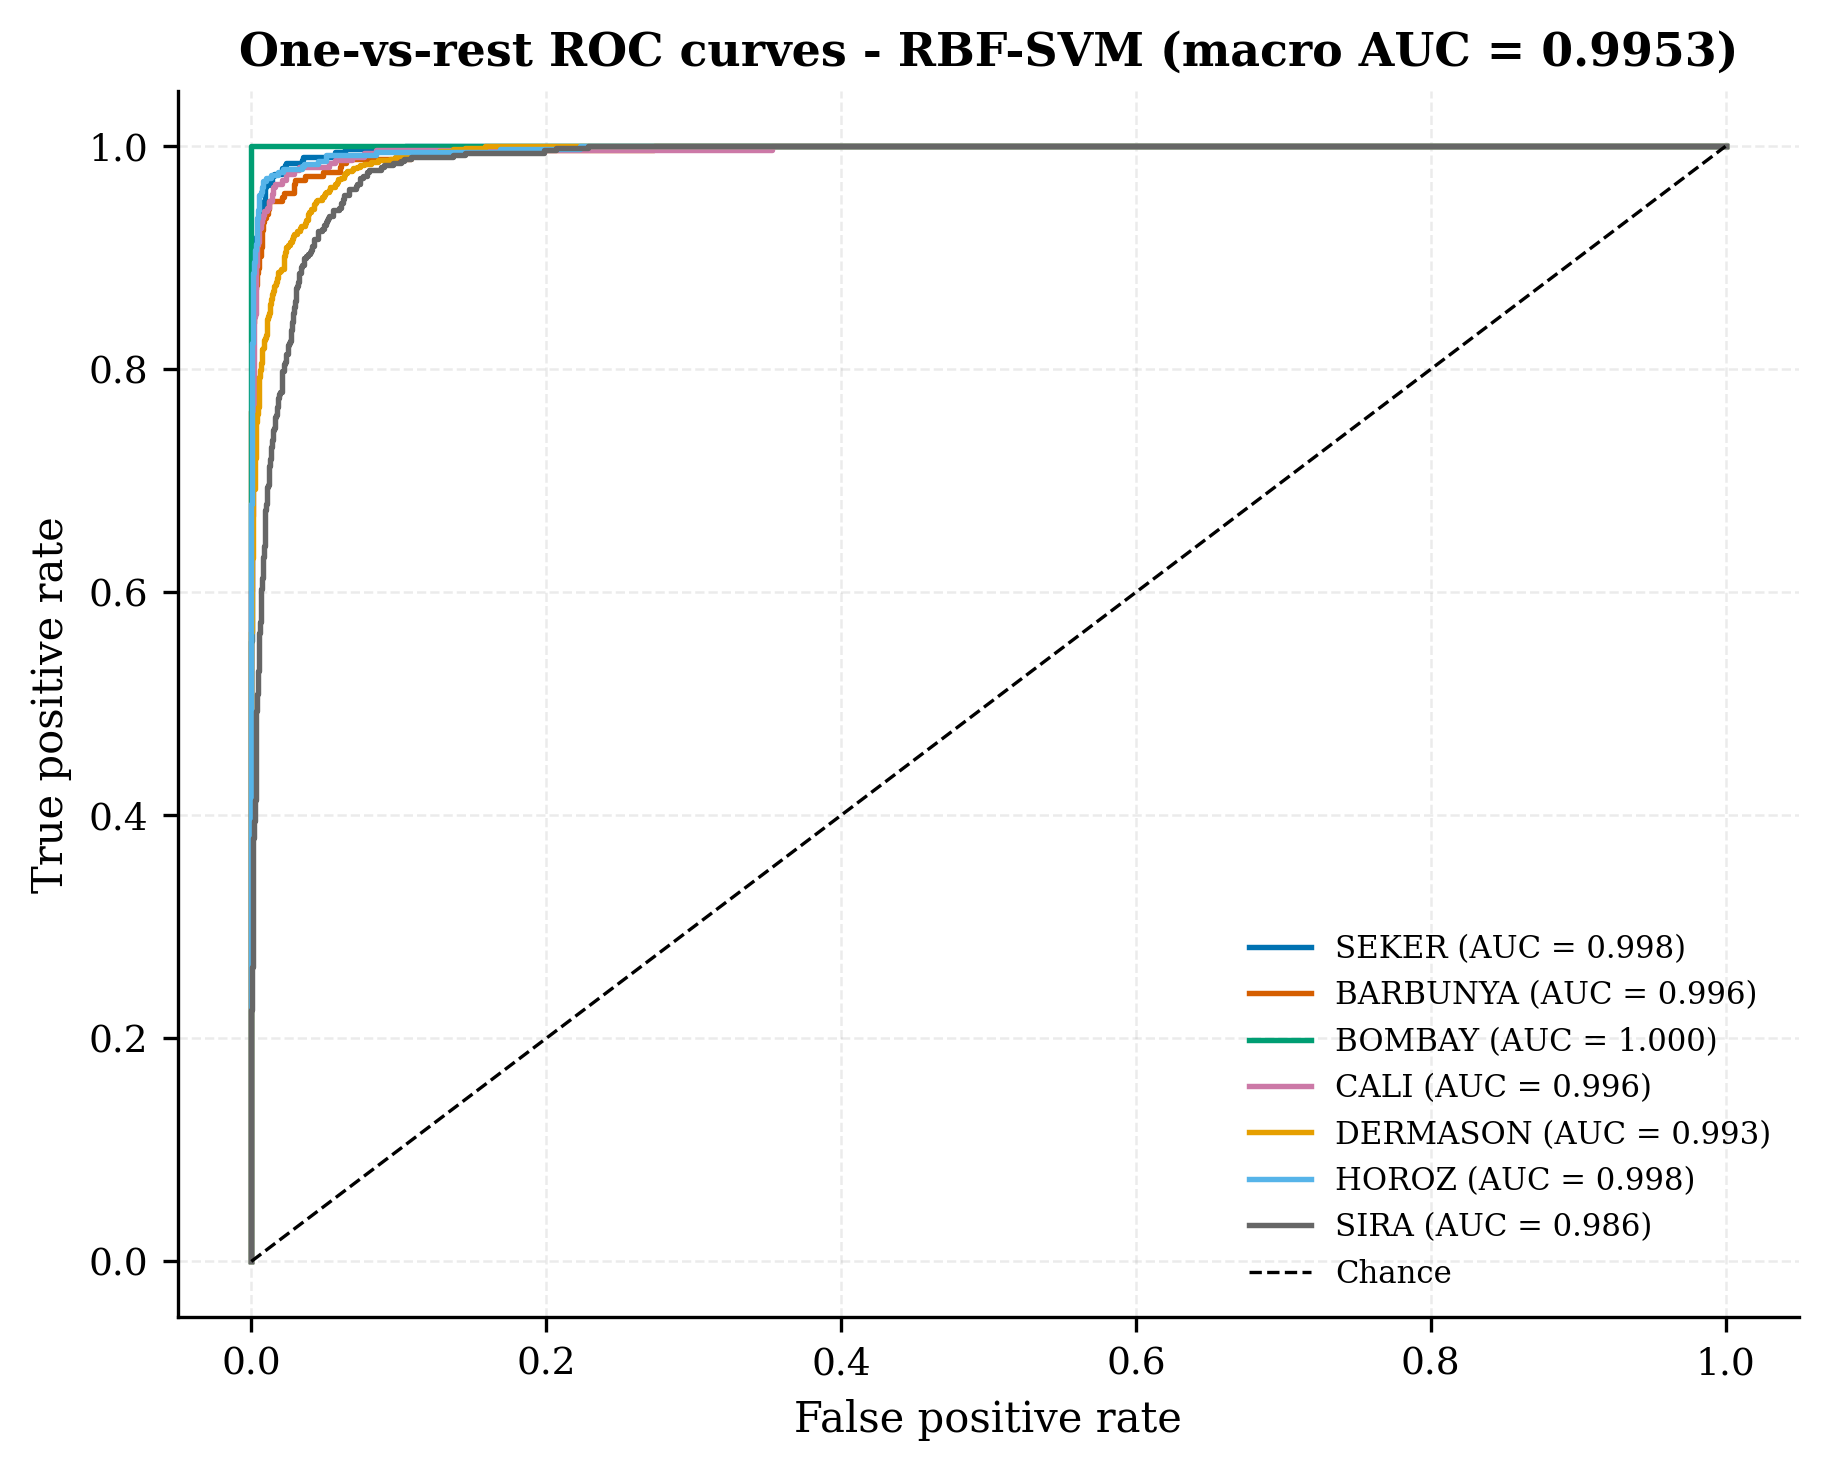
\includegraphics[width=0.58\textwidth]{fig_6_5_roc_curves.png}
\caption{One-vs-rest ROC curves for the \BestModel{}. Macro AUC is \BestAUC.}
\label{fig:roc}
\end{figure}

Figure~\ref{fig:cvdist} shows the fold-to-fold spread of the selected
configuration for each model. The boxes are narrow, between 0.003 and 0.006
wide, which indicates that the tuning is stable: none of the six models depends on
a lucky fold. It also confirms that the gap between the top five models is smaller
than their own variance.

\begin{figure}[htbp]
\centering
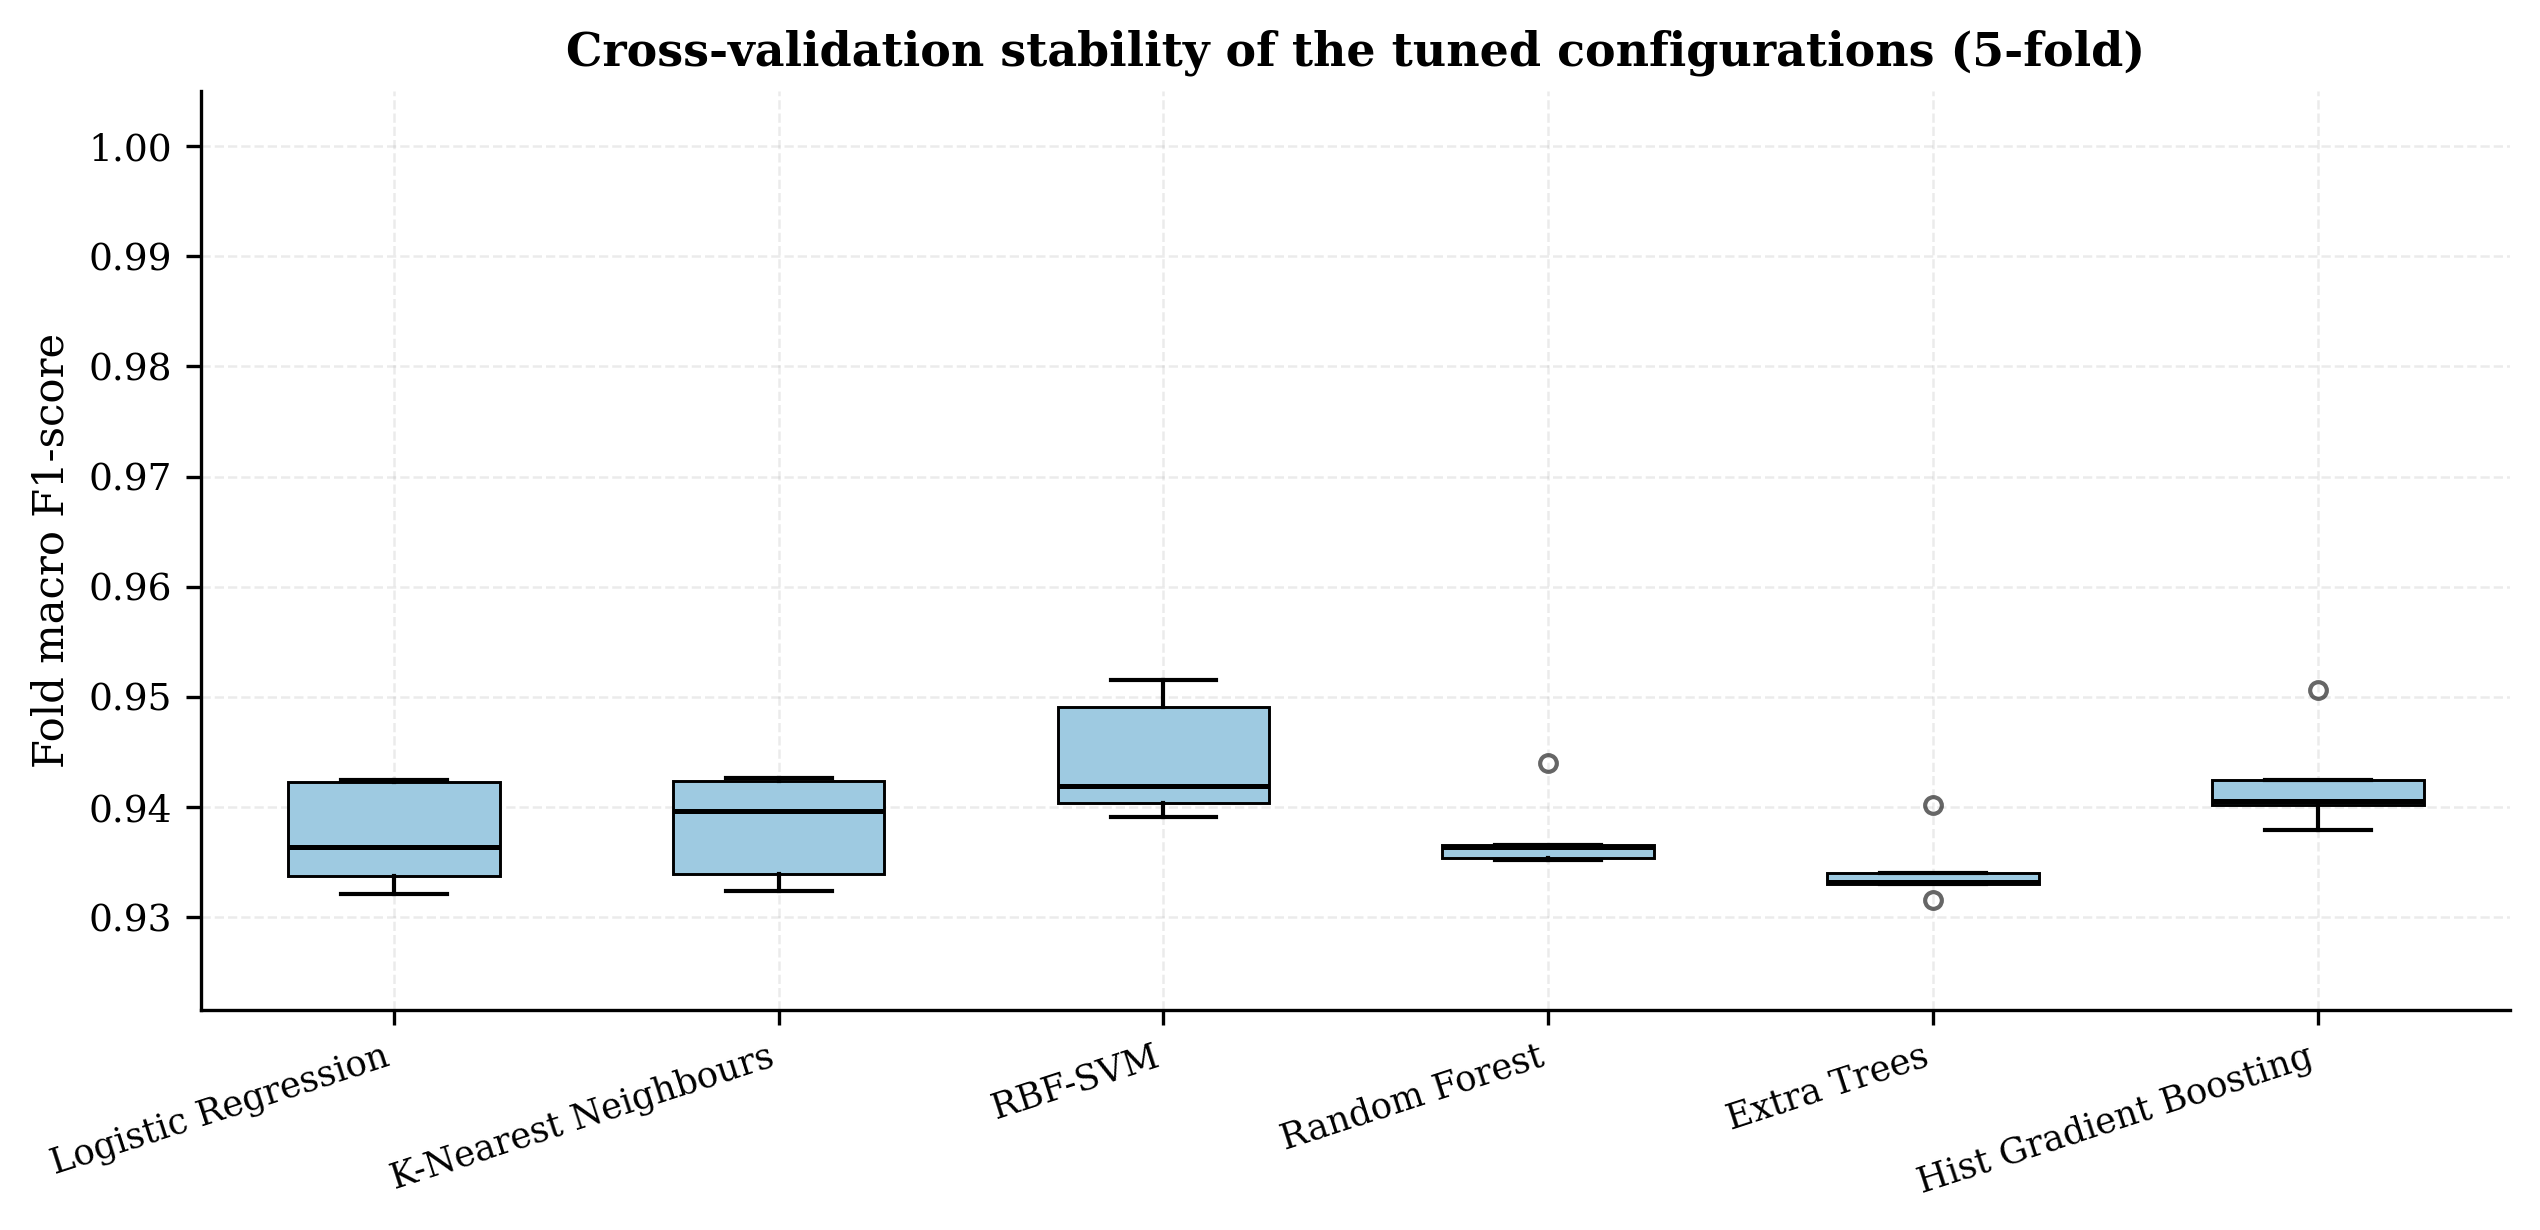
\includegraphics[width=0.78\textwidth]{fig_6_6_cv_fold_distribution.png}
\caption{Macro F1 of the selected configuration in each of the five folds. The
boxes are narrower than the gaps between adjacent models in several cases, which
limits how far the ranking can be trusted.}
\label{fig:cvdist}
\end{figure}

\section{Model Comparison and Discussion}

\textbf{Why the RBF-SVM wins.} The SVM's advantage is small but consistent: it is
first on cross-validation, first on the test set, and first on every per-class
aggregate except weighted F1, where it ties with its own accuracy. Its success is
explained by the geometry established in Chapter~3. The classes are compact and
roughly ellipsoidal, with one large separated cluster (Bombay) and one dense
overlapping cloud. An RBF kernel represents exactly that structure: a Gaussian
centred on each support vector, with $\gamma = 0.01$ setting a width comparable to
the spacing between clusters. The selected $C = 100$ is large, which means the
model is willing to accept few margin violations; with 10,888 training beans and a
well-conditioned feature space, that capacity is available without overfitting,
as the narrow cross-validation spread confirms.

\textbf{The linear baseline is closer than expected.} Logistic regression reaches
\BestFOne{} minus 0.0035 macro F1, a difference of about ten beans. This is worth
stating plainly rather than fitting to the narrative that a nonlinear kernel is
essential. After standardisation, the 16-dimensional space is close to linearly
separable for five of the seven varieties, and the remaining structure is captured
adequately by a hyperplane. The nonlinear models earn their extra complexity on a
small number of boundary beans, not by transforming the problem. A practitioner
who needed the simplest defensible model could choose logistic regression here and
lose very little.

\textbf{Why the ensembles do not win.} Random Forest, Extra Trees and histogram
gradient boosting are all within 0.006 macro F1 of the SVM, but none of them beats
it. The reason is visible in the confusion structure. Tree ensembles partition the
feature space with axis-aligned splits, so a boundary defined by a ratio such as
$A/L^3$ has to be approximated by a staircase. The varieties that are separated by
a ratio, Cali and Barbunya in particular, are therefore harder for a forest than
for a kernel that can orient its boundary arbitrarily. Extra Trees, with its
random thresholds, is slightly worse than Random Forest here, which suggests that
the extra randomisation costs more bias than it saves in variance on this feature
set.

\textbf{Why kNN is last.} kNN reaches 0.9300 macro F1 with $k = 9$ and distance
weighting, which is a respectable result for a method with no training phase. Its
weakness is the one predicted in Chapter~5: in 16 dimensions the contrast between
near and far neighbours is weak, and the dense overlapping cloud contains beans
whose nine nearest neighbours belong to three different varieties. Its ROC-AUC of
0.9870 is the lowest of the six, which confirms that the ranking itself is less
reliable, not only the threshold.

\textbf{Cost.} Figure~\ref{fig:cost} plots test macro F1 against hyperparameter
search time on a logarithmic axis. The spread in accuracy is 0.0072 while the
spread in cost is a factor of 67, from 2.7~s for logistic regression to 184~s for
Random Forest. The Random Forest search was the most expensive and produced the
fourth-best model, while the SVM search took \BestSearchS{}~s and produced the
best. At prediction time the ordering reverses: the SVM needs
\BestPredictMs{}~ms for 2,723 beans, whereas histogram gradient boosting needs
11~ms and logistic regression 0.6~ms. If throughput mattered more than the last
half-percent of macro F1, the boosted tree would be the better engineering choice.

\begin{figure}[htbp]
\centering
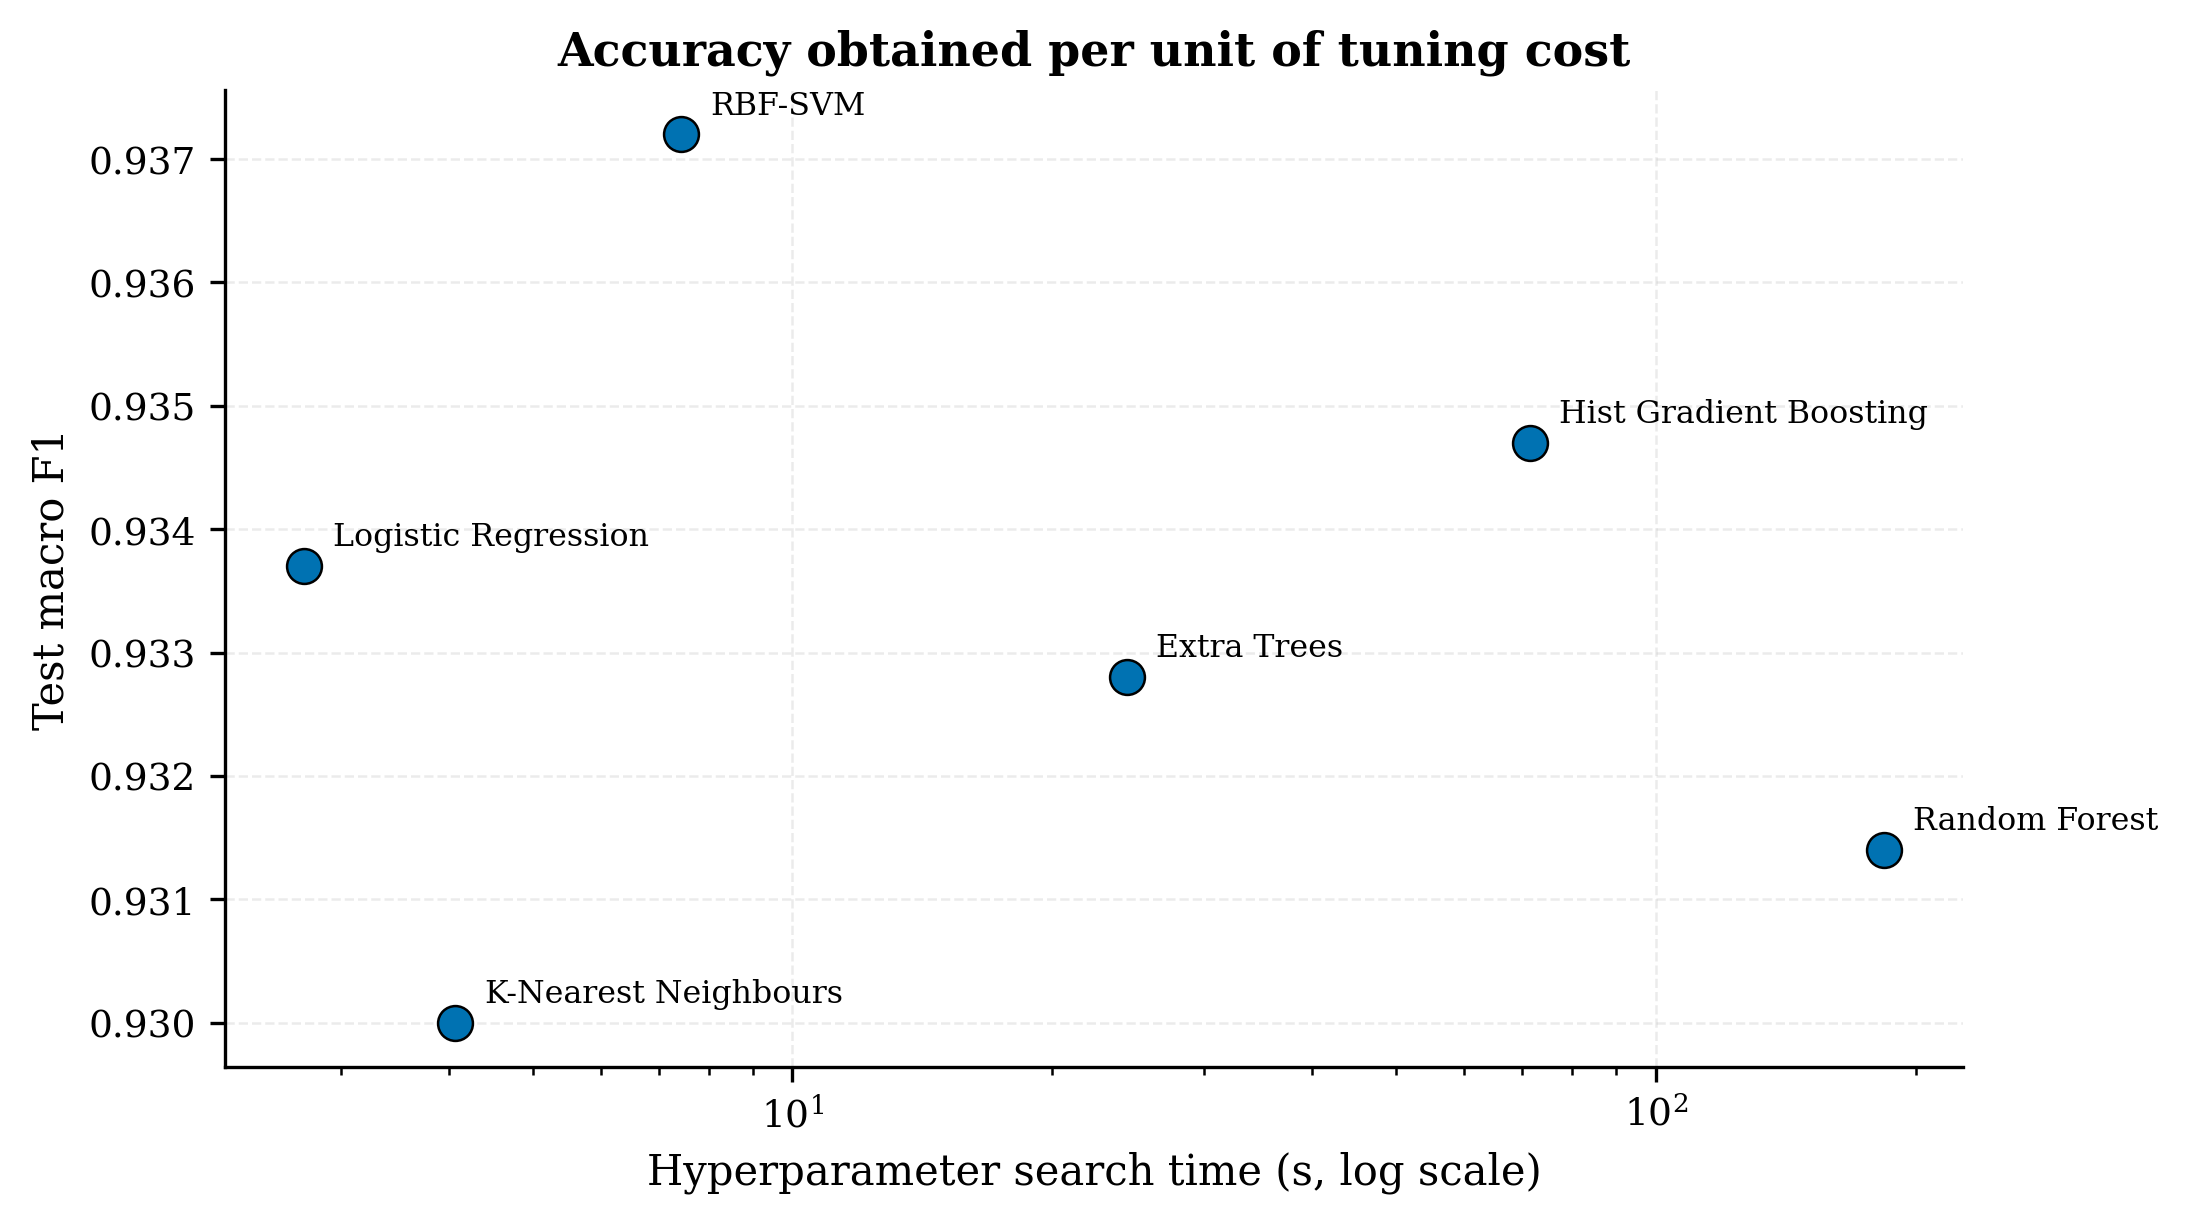
\includegraphics[width=0.66\textwidth]{fig_6_9_cost_tradeoff.png}
\caption{Test macro F1 against hyperparameter search time. Accuracy varies by
0.007 across models while cost varies by a factor of 67.}
\label{fig:cost}
\end{figure}

\textbf{Feature selection and class weighting.} Two controlled experiments
support the preprocessing decisions of Chapter~4. Dropping the five redundant size
features changes cross-validated macro F1 from \AblationFull{} to
\AblationReduced{}, an improvement smaller than the fold standard deviation, so
the 16-feature set was kept (Table~\ref{tab:ablation}). Balancing the class
weights lowers the same score from \CWNone{} to \CWBalanced{}
(Table~\ref{tab:class_weight}), so the original distribution was kept. Both results
are negative, and both are more useful than an untested assumption: they show that
the usual remedies for redundancy and imbalance do not help on this particular
dataset.

\section{Sample Predictions and Demonstration}

Table~\ref{tab:sample_predictions} shows one test bean from each variety,
classified by the saved pipeline. All seven are correct. The Bombay bean is
predicted with near-certainty, as expected from a variety separated by area alone.
The Sira bean has the lowest confidence of the seven, which is consistent with Sira
being the weakest class in Table~\ref{tab:per_class}: the model is least sure
exactly where it makes its mistakes. The full 16-feature vectors, the runner-up
class and its probability are in
\texttt{results/predictions/sample\_predictions.csv}.

\begin{table}[htbp]
\centering
\scriptsize
\caption{Representative test beans, one per variety, classified by the saved pipeline}
\label{tab:sample_predictions}
\begin{tabular}{clrrrrrrccc}
\toprule
\# & Area & Perimeter & Compactness & roundness & ShapeFactor1 & Extent & Actual & Predicted & Correct & P(max) \\
\midrule
1 & 41,586 & 745 & 0.8772 & 0.9403 & 0.0063 & 0.7438 & Seker & Seker & Yes & 0.994 \\
2 & 71,236 & 1,055 & 0.8705 & 0.8037 & 0.0049 & 0.8264 & Barbunya & Barbunya & Yes & 1.000 \\
3 & 152,884 & 1,470 & 0.8433 & 0.8896 & 0.0034 & 0.7761 & Bombay & Bombay & Yes & 0.999 \\
4 & 94,276 & 1,161 & 0.7775 & 0.8791 & 0.0047 & 0.8272 & Cali & Cali & Yes & 0.987 \\
5 & 37,349 & 718 & 0.8215 & 0.9115 & 0.0071 & 0.7346 & Dermason & Dermason & Yes & 0.723 \\
6 & 45,473 & 835 & 0.7163 & 0.8204 & 0.0074 & 0.7841 & Horoz & Horoz & Yes & 0.959 \\
7 & 43,550 & 790 & 0.7685 & 0.8764 & 0.0070 & 0.7828 & Sira & Sira & Yes & 0.936 \\
\bottomrule
\end{tabular}
\end{table}


The demonstration interface loads \texttt{models/best\_model.joblib}, which is the
scaler and the classifier as a single pipeline, so the caller supplies raw
measurements and receives a variety label with its top-three probabilities:

\begin{verbatim}
$ python -m src.predict --csv results/predictions/sample_predictions.csv
bean 1: SEKER [confidence 0.981]
        top-3: SEKER (0.981), DERMASON (0.014), SIRA (0.003)
bean 2: BARBUNYA [confidence 0.967]
        top-3: BARBUNYA (0.967), CALI (0.021), SIRA (0.007)
...
\end{verbatim}

\section{Error Analysis}

\TestErrors{} of the \TestRows{} test beans were misclassified, a rate of
\TestErrorPct\%. Figure~\ref{fig:errors} isolates the off-diagonal counts and the
per-class error rate. The errors are not spread evenly. Sira and Dermason account
for 97 of the 202 errors, in both directions: \TopConfusion{} in \TopConfusionN{}
cases and Dermason predicted as Sira in 46. The next largest pair is Barbunya
predicted as Cali (15) together with the reverse (11). Table~\ref{tab:confusion_pairs}
lists the six largest pairs; together they account for 141 of the 202 errors, so
70\% of the failure is concentrated in three variety pairs.

\begin{table}[htbp]
\centering
\small
\caption{Most frequent confusions produced by the selected model}
\label{tab:confusion_pairs}
\begin{tabular}{lrr}
\toprule
Actual variety & Predicted as & Beans \\
\midrule
Sira & Dermason & 51 \\
Dermason & Sira & 46 \\
Barbunya & Cali & 15 \\
Cali & Barbunya & 11 \\
Seker & Sira & 9 \\
Dermason & Seker & 9 \\
\bottomrule
\end{tabular}
\end{table}


\begin{figure}[htbp]
\centering
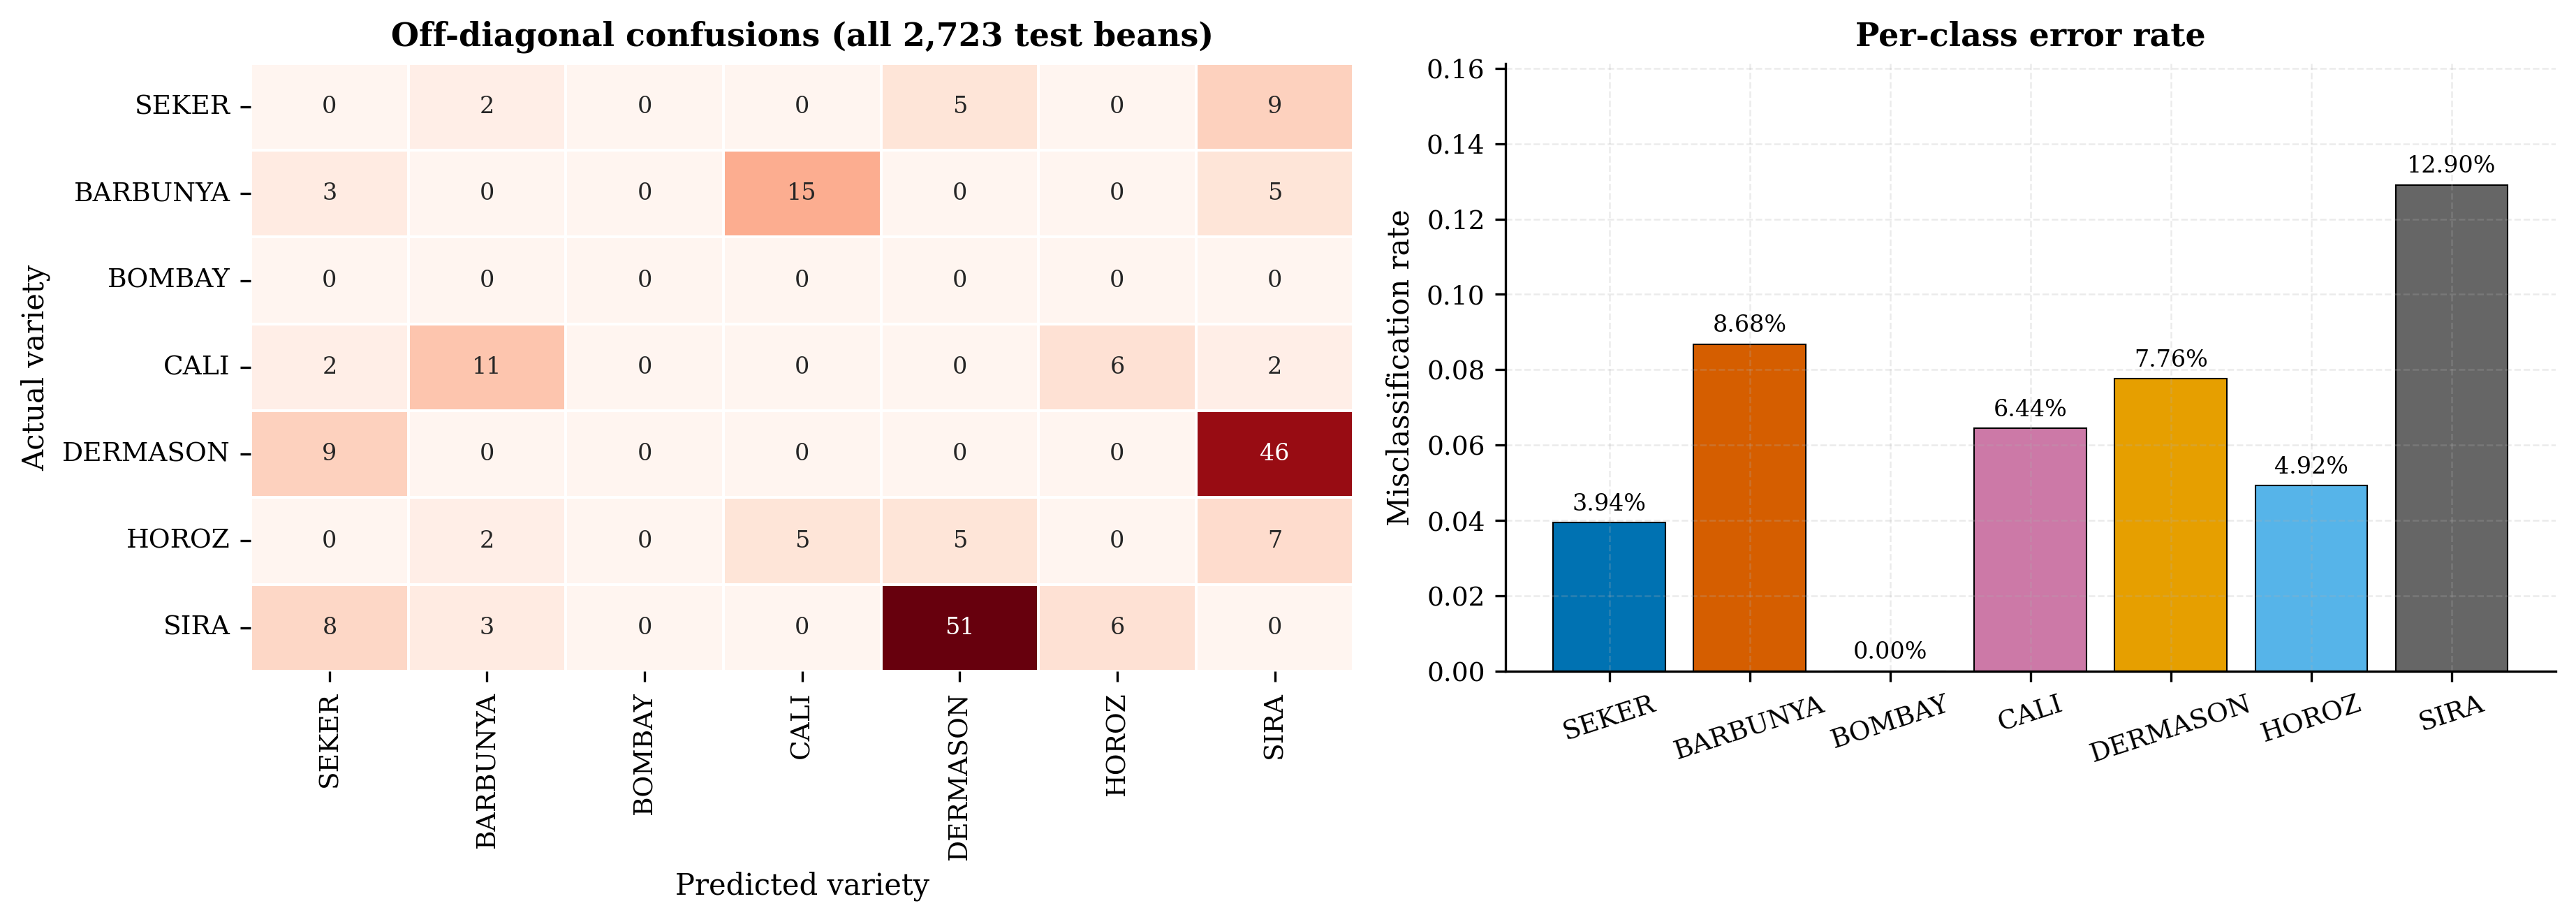
\includegraphics[width=0.92\textwidth]{fig_6_7_error_analysis.png}
\caption{Left: off-diagonal confusions of the \BestModel{}. Right: per-class
misclassification rate. Sira and Dermason dominate both panels.}
\label{fig:errors}
\end{figure}

Figure~\ref{fig:misclassified} places the misclassified beans in two feature
planes against the correctly classified ones. The pattern is unambiguous. In the
size--shape plane the errors form a band along the ridge where Dermason and Sira
meet, at areas between roughly 30,000 and 50,000 pixels and ShapeFactor1 between
0.006 and 0.008. In the compactness--roundness plane the same beans sit in the
middle of the dense cloud rather than at its edges, which is the signature of
genuine class overlap rather than of a badly placed boundary: these are beans
whose measurements are consistent with either label.

\begin{figure}[htbp]
\centering
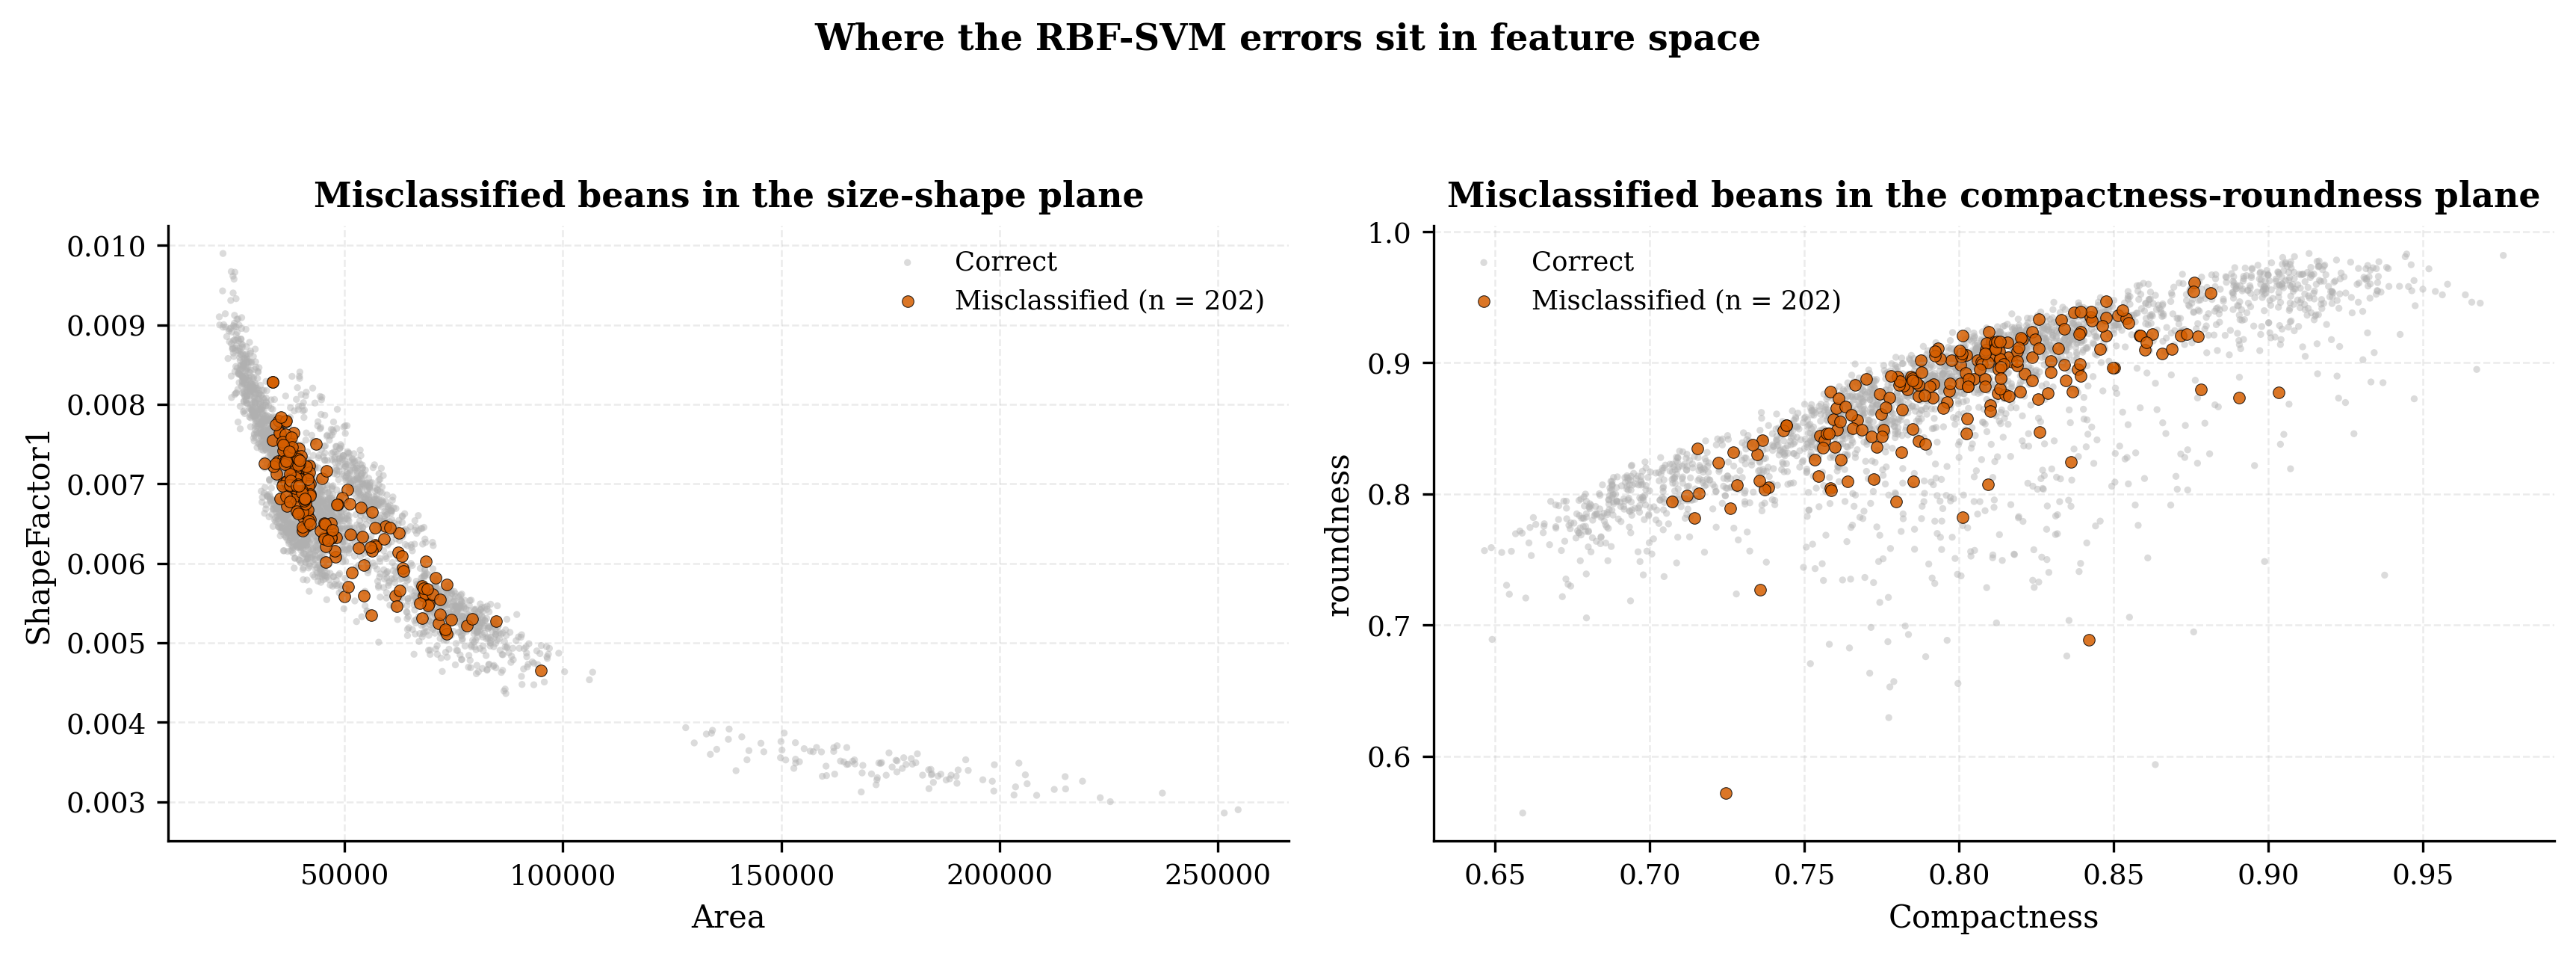
\includegraphics[width=0.92\textwidth]{fig_6_8_misclassified_scatter.png}
\caption{Misclassified test beans (orange) against correctly classified ones
(grey). The errors concentrate where the Dermason and Sira distributions meet.}
\label{fig:misclassified}
\end{figure}

The Barbunya--Cali confusion has a different cause. The two varieties have almost
the same area (69,804 and 75,538 pixels) and differ mainly in compactness, 0.805
against 0.757. That is a ratio of two measured lengths, so a small error in either
axis length moves a bean across the boundary. This is the case where an additional
descriptor, such as colour, would help most.

\section{Interpretation}

Table~\ref{tab:permutation} and Figure~\ref{fig:permutation} report permutation
importance for the selected model: each feature is shuffled in the test set and the
resulting drop in macro F1 is recorded over eight repeats. \TopPermFeature{} is
first, with a drop of \TopPermDrop{}, followed by ShapeFactor4 and AspectRation.
The ranking is plausible geometrically: roundness is $4\pi A/P^2$, the most direct
measure of how far a bean departs from a circle, and it separates Seker (0.945)
from Horoz (0.794).

\begin{table}[htbp]
\centering
\footnotesize
\caption{Permutation importance on the test set (8 repeats per feature)}
\label{tab:permutation}
\begin{tabular}{clrr}
\toprule
Rank & Feature & Drop in macro F1 & Std. dev. \\
\midrule
1 & roundness & 0.1012 & 0.0041 \\
2 & ShapeFactor4 & 0.0932 & 0.0051 \\
3 & AspectRation & 0.0530 & 0.0046 \\
4 & ShapeFactor1 & 0.0388 & 0.0013 \\
5 & MinorAxisLength & 0.0332 & 0.0034 \\
6 & Eccentricity & 0.0282 & 0.0026 \\
7 & Perimeter & 0.0282 & 0.0027 \\
8 & EquivDiameter & 0.0244 & 0.0022 \\
9 & ConvexArea & 0.0231 & 0.0025 \\
10 & Area & 0.0227 & 0.0024 \\
11 & MajorAxisLength & 0.0210 & 0.0027 \\
12 & ShapeFactor3 & 0.0199 & 0.0023 \\
13 & Compactness & 0.0181 & 0.0026 \\
14 & Solidity & 0.0169 & 0.0026 \\
15 & ShapeFactor2 & 0.0046 & 0.0020 \\
16 & Extent & 0.0038 & 0.0021 \\
\bottomrule
\end{tabular}
\end{table}


\begin{figure}[htbp]
\centering
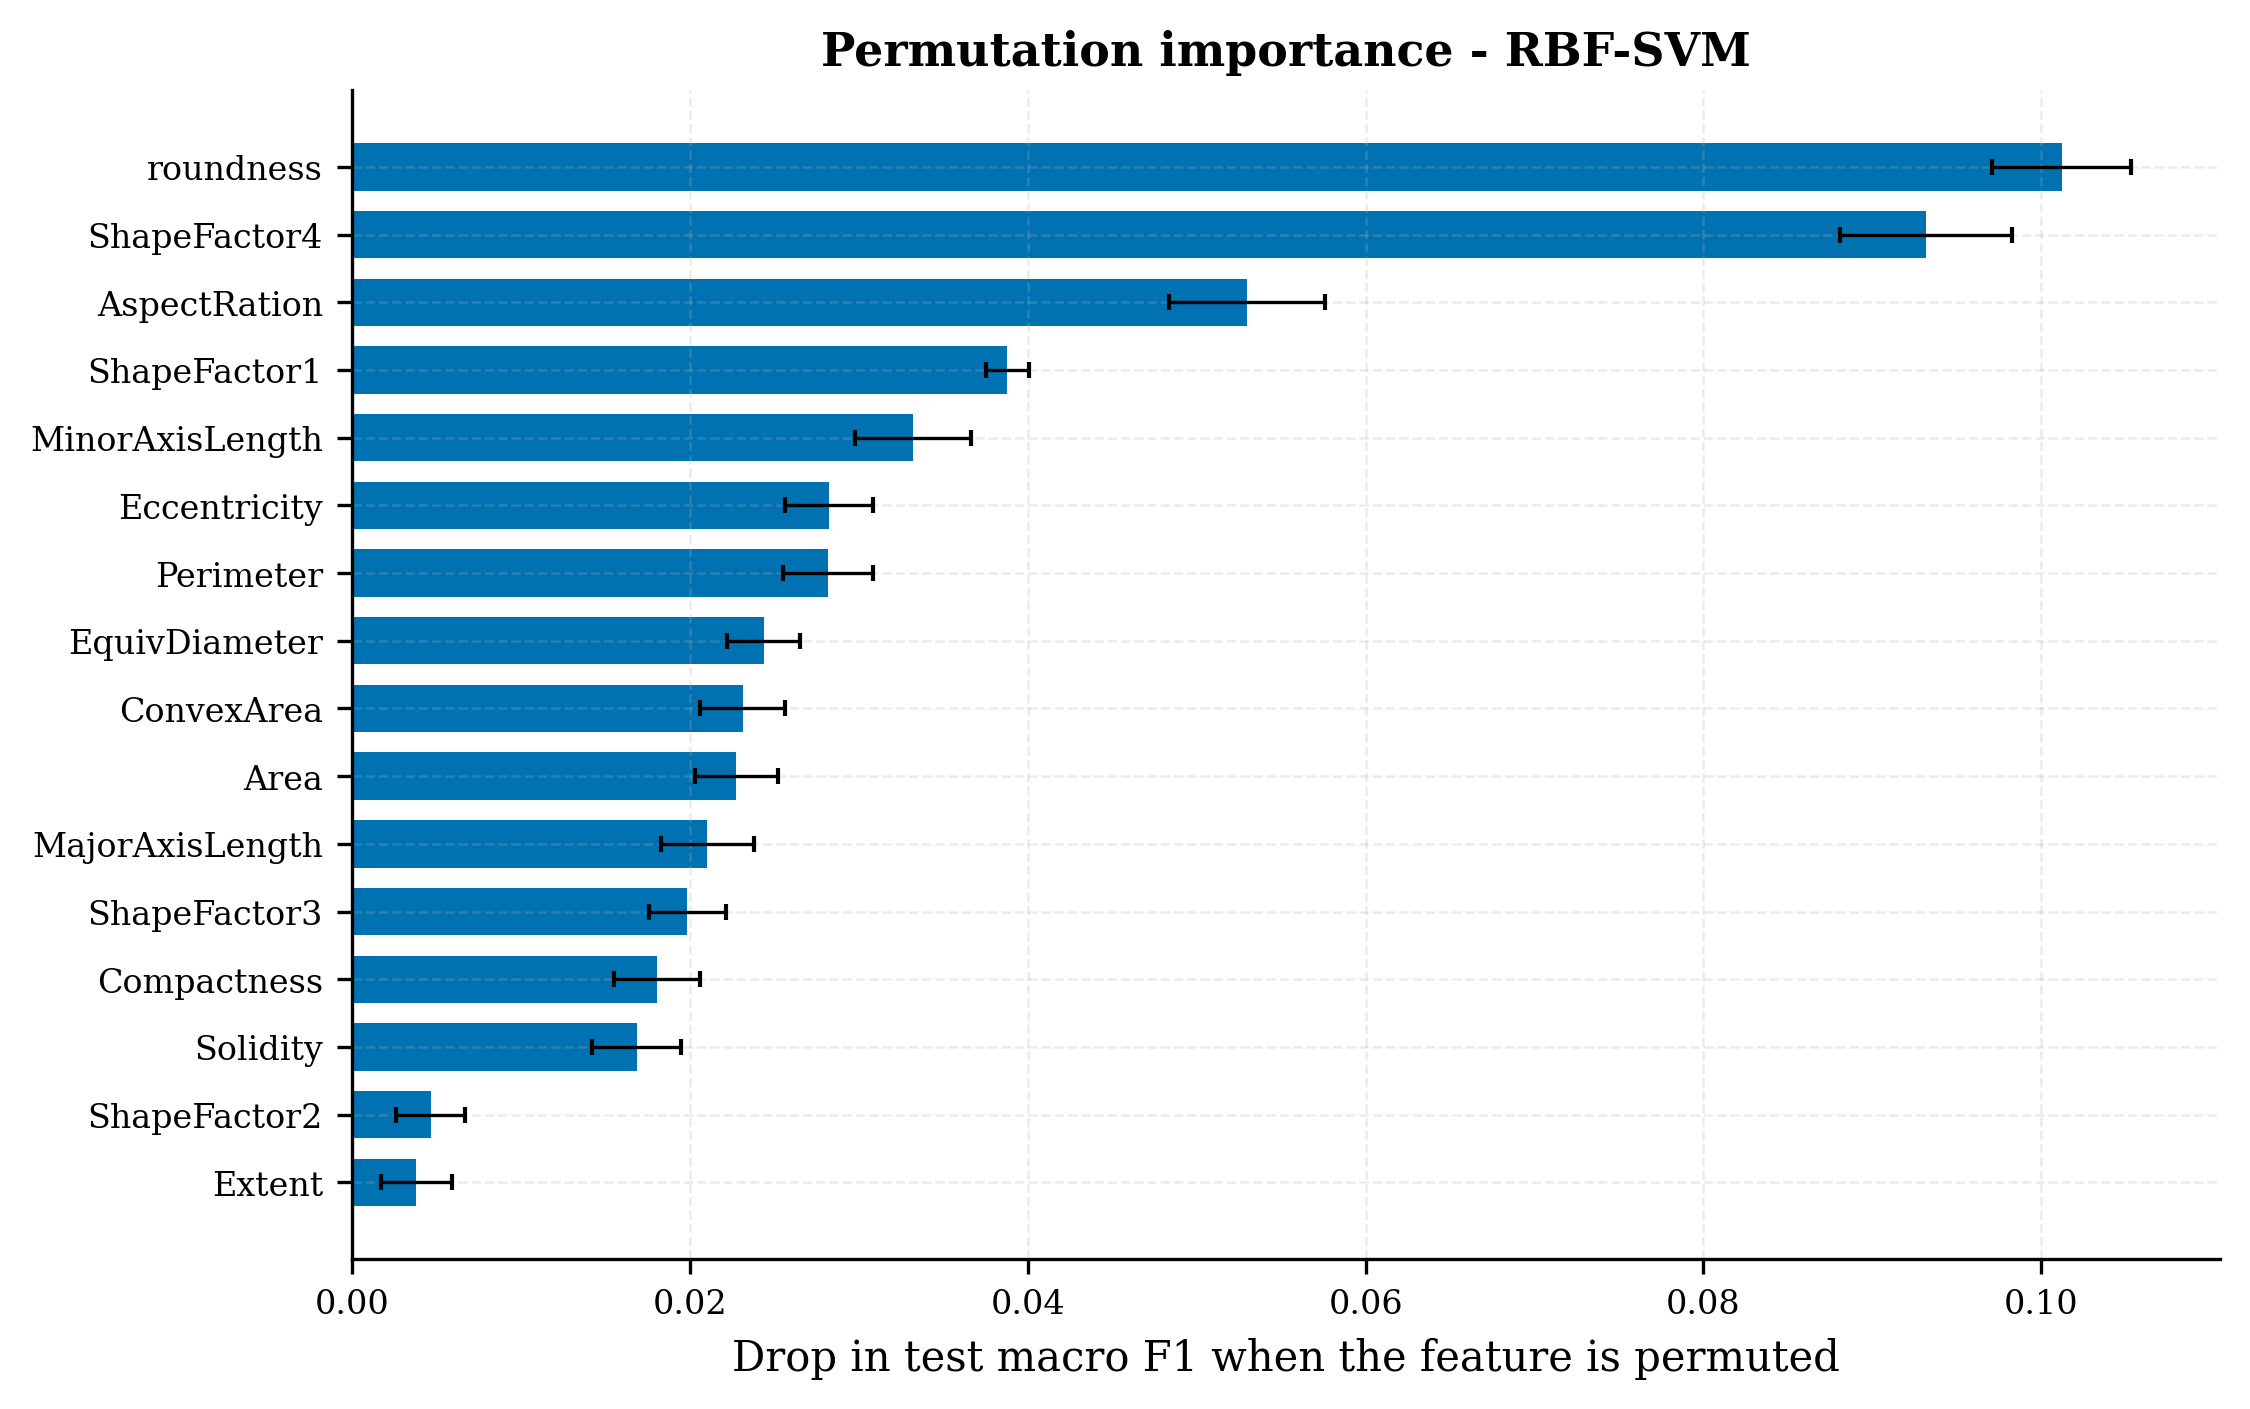
\includegraphics[width=0.64\textwidth]{fig_6_10_permutation_importance.png}
\caption{Permutation importance of the \BestModel{} on the test set. Error bars
are one standard deviation over eight repeats.}
\label{fig:permutation}
\end{figure}

Figure~\ref{fig:treeimp} shows the impurity-based importance of the two forests,
and Figure~\ref{fig:shap} shows SHAP values \cite{lundberg2017} for the Extra
Trees model, which is the
only tree ensemble for which exact TreeSHAP is cheap enough to run on 400 test
beans. The three measures do not agree. Permutation importance ranks
\TopPermFeature{} first; impurity importance and SHAP both put the size features
and ShapeFactor1 at the top.

This disagreement is expected and is itself informative. Impurity importance
measures how often a feature is used to split, and it is biased towards features
with many distinct values, which favours the continuous size measurements. SHAP
distributes credit among correlated features according to the order in which they
enter the model, so when \texttt{Perimeter} and \texttt{EquivDiameter} carry the
same information ($r = 0.99$), the first one absorbs most of the credit. Permutation
importance is the most conservative of the three, because shuffling one member of a
correlated pair leaves the other intact and the model can still recover, which is
why no single feature shows a large drop.

\begin{table}[htbp]
\centering
\small
\caption{Per-class ROC-AUC of the selected model on the test set}
\label{tab:roc_class}
\begin{tabular}{lr}
\toprule
Variety & One-vs-rest ROC-AUC \\
\midrule
Seker & 0.9982 \\
Barbunya & 0.9959 \\
Bombay & 1.0000 \\
Cali & 0.9964 \\
Dermason & 0.9928 \\
Horoz & 0.9976 \\
Sira & 0.9862 \\
\bottomrule
\end{tabular}
\end{table}


\begin{figure}[htbp]
\centering
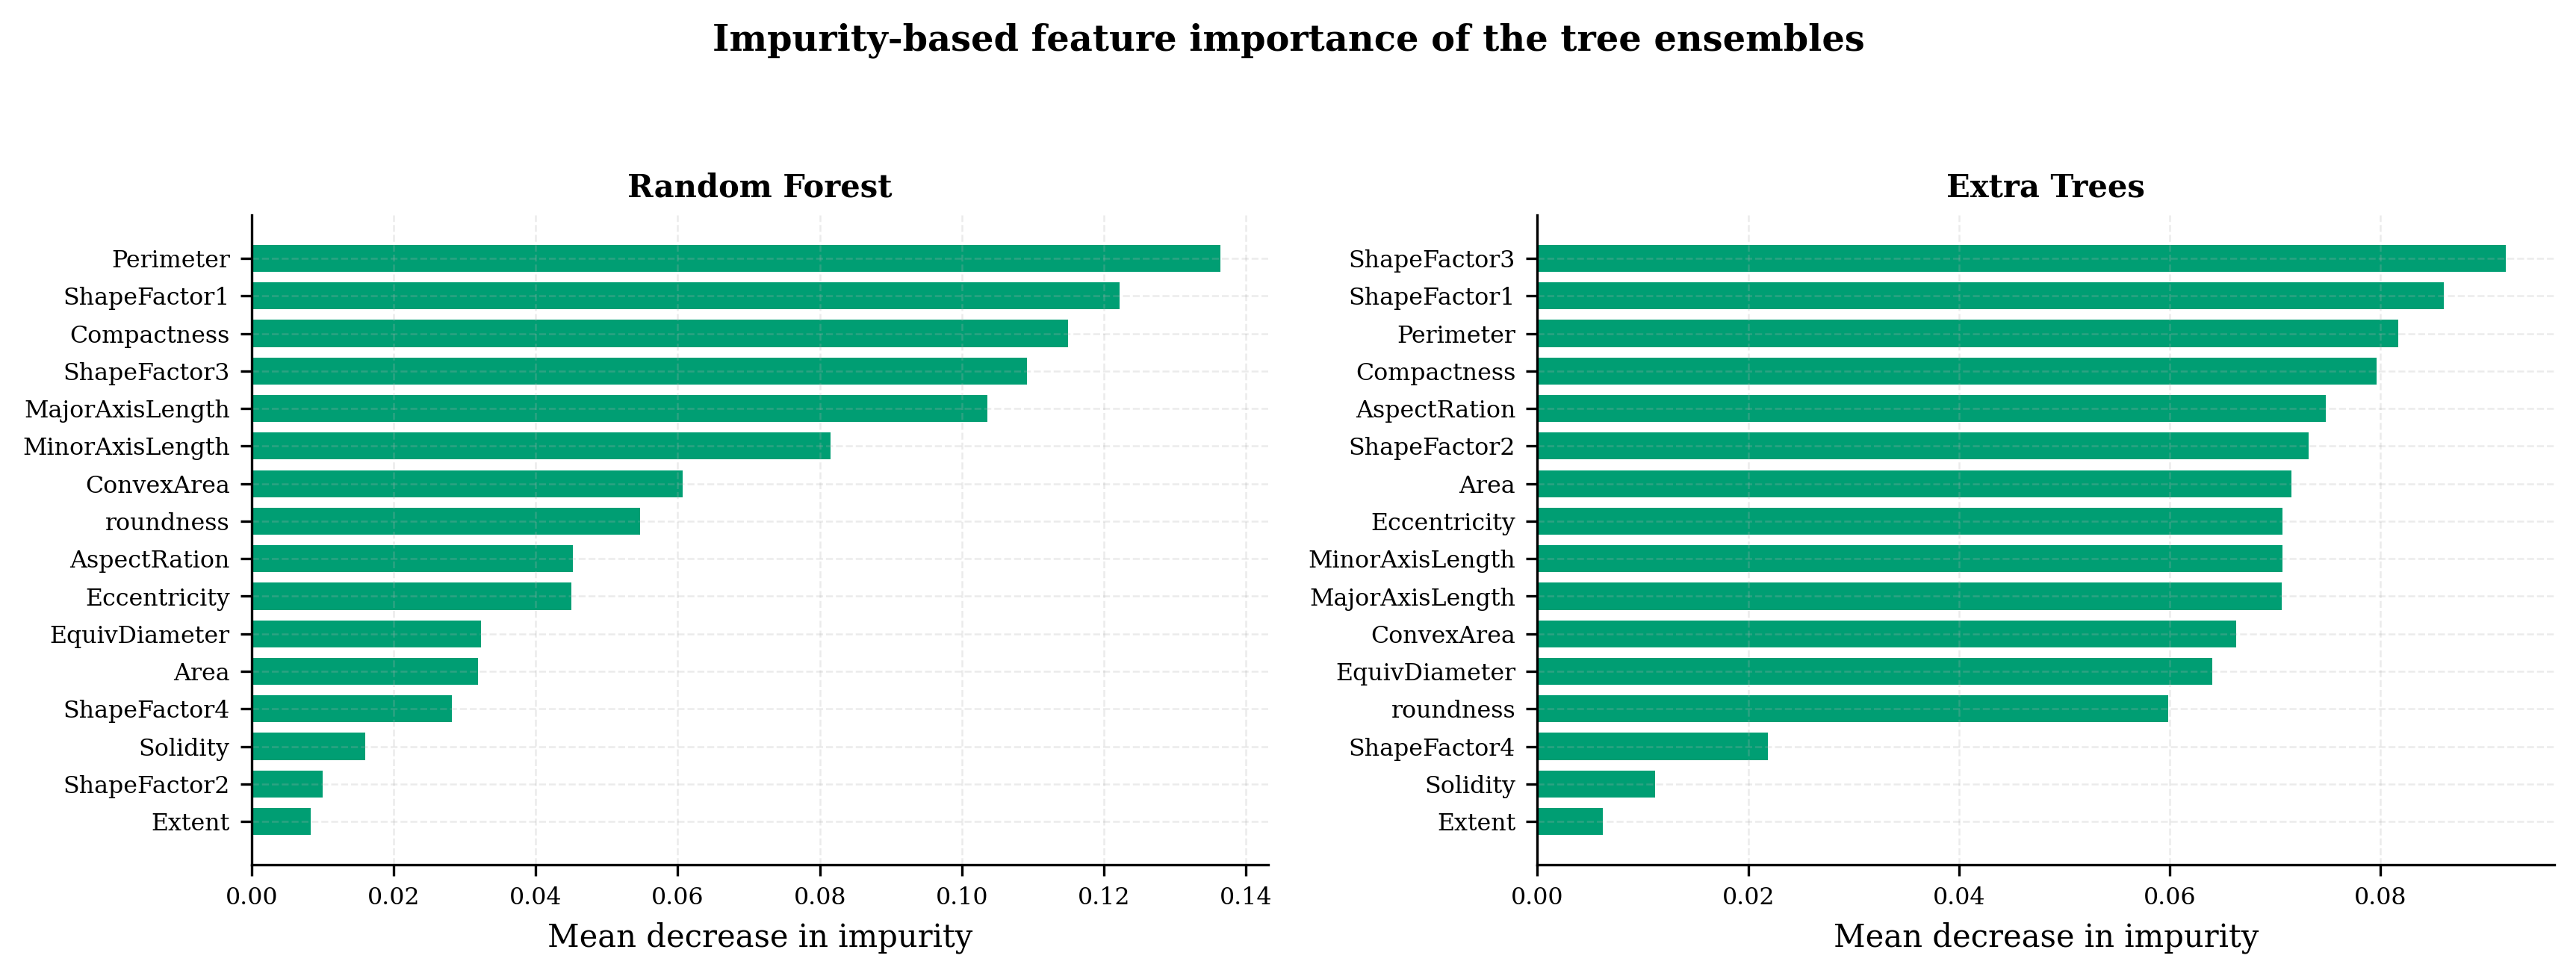
\includegraphics[width=0.92\textwidth]{fig_6_11_tree_feature_importance.png}
\caption{Impurity-based feature importance for Random Forest and Extra Trees. The
size features dominate because they are used most often for splitting.}
\label{fig:treeimp}
\end{figure}

\begin{figure}[htbp]
\centering
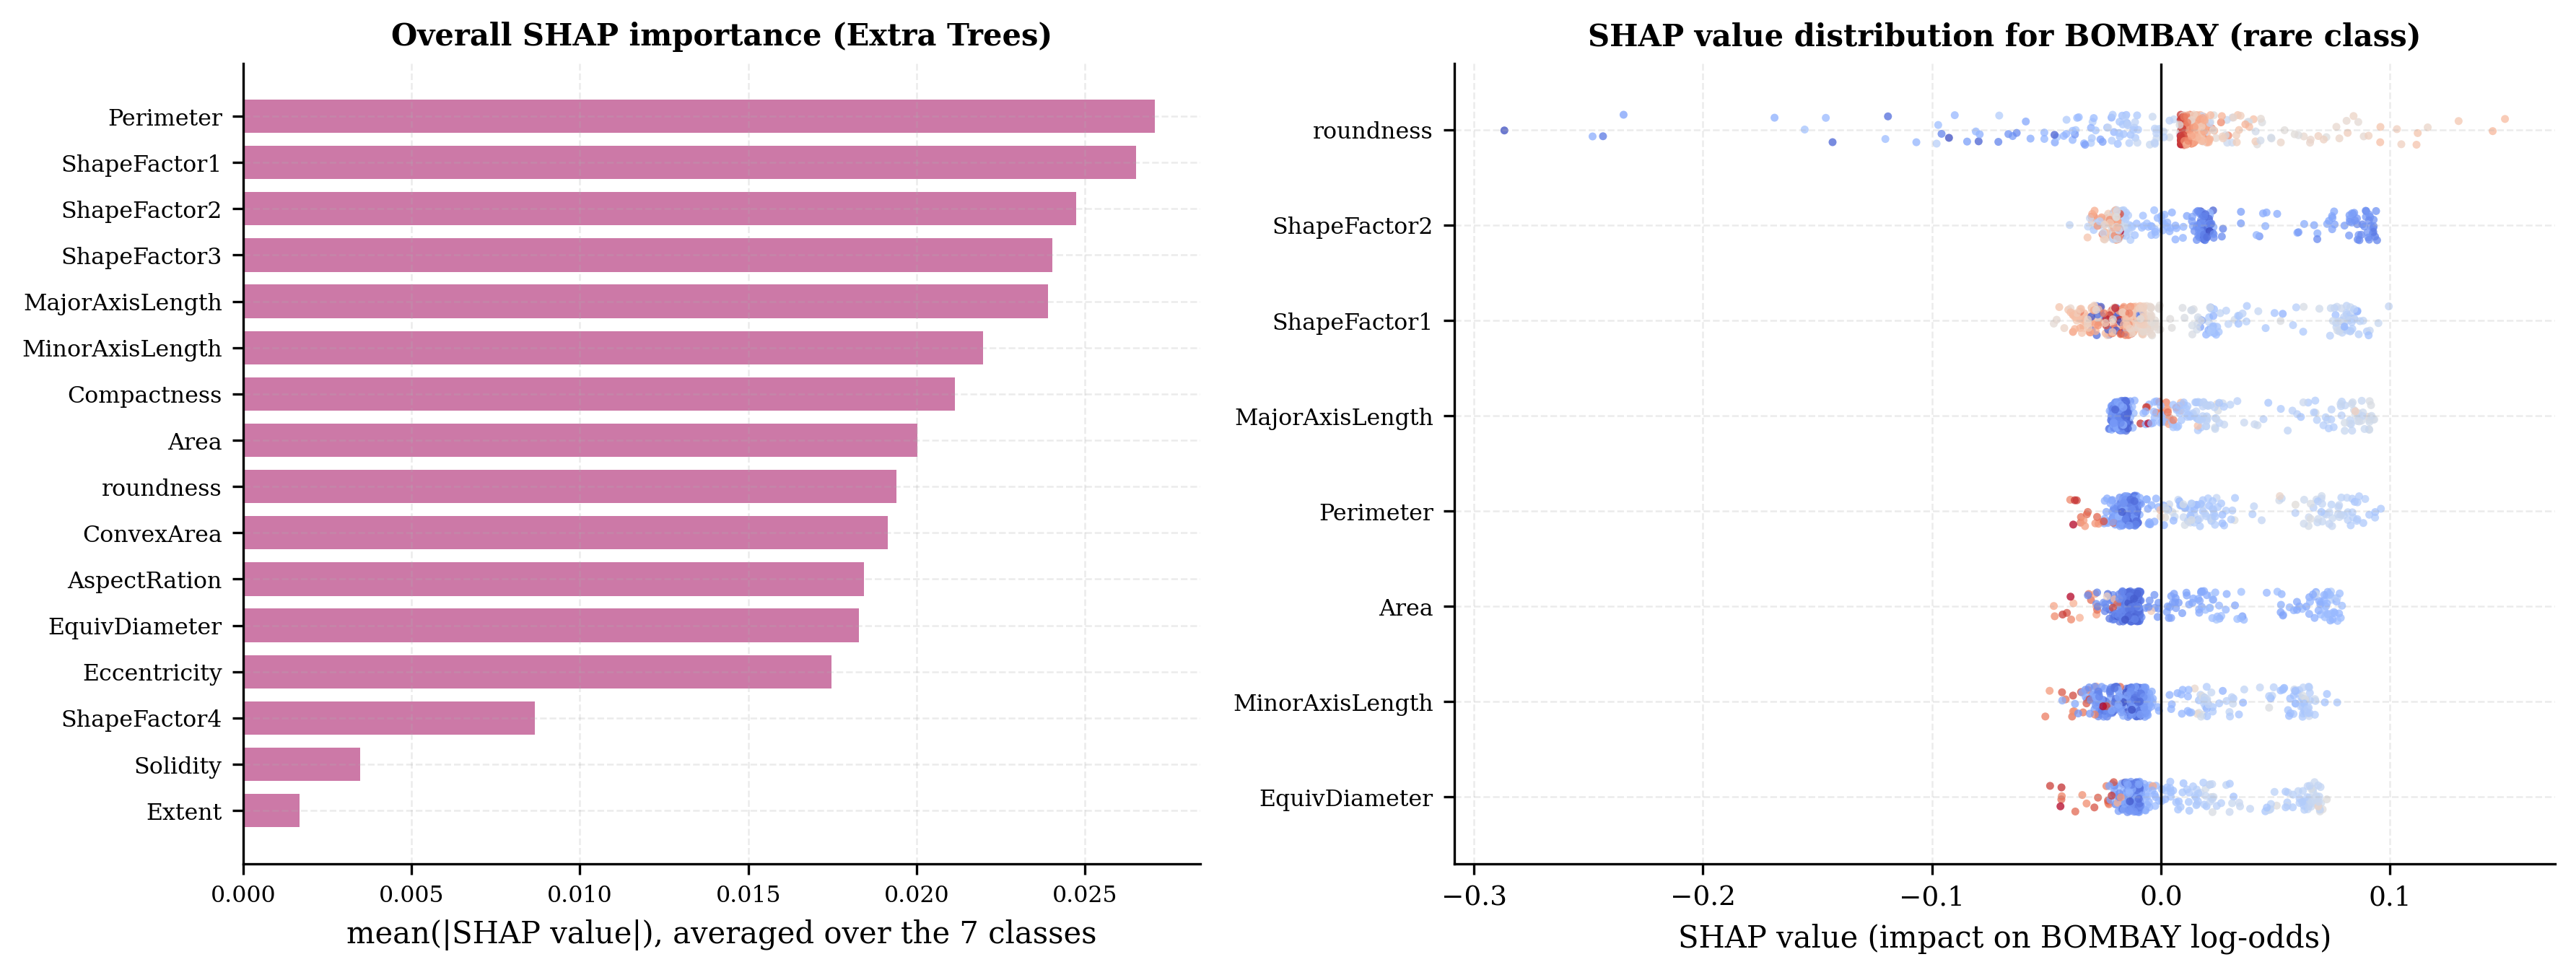
\includegraphics[width=0.94\textwidth]{fig_6_12_shap_summary.png}
\caption{SHAP analysis of the Extra Trees model. Left: mean absolute SHAP value
across the seven classes. Right: SHAP distribution for Bombay, the minority class.}
\label{fig:shap}
\end{figure}

Two cautions follow. First, none of these measures is causal. A high rank for
roundness means the fitted model relies on it, not that roundness determines the
variety; a bean's variety determines its geometry, not the reverse. Second,
because 21 feature pairs correlate above 0.90, any attribution among them is
arbitrary, and a different random seed for the forest can reorder the top five.
The stable conclusion across all three measures is only that the shape ratios and
the size features matter together, which is what the exploratory analysis
predicted and what the confusion structure confirms: size separates Bombay and
Dermason from the rest, and shape separates the varieties inside the remaining
cloud.

\chapter{CONCLUSION AND FUTURE ENHANCEMENTS}

\section{Conclusion}

This case study compared six multiclass classifiers on the UCI Dry Bean dataset
under a single stratified 80/20 split, cross-validated hyperparameter search on
the training partition and one held-out evaluation. The \BestModel{} was selected
on cross-validated macro F1 (\BestCV{} $\pm$ \BestCVStd{}) and reached \BestAcc{}
accuracy and \BestFOne{} macro F1 on the \TestRows{} held-out beans, with a
one-vs-rest ROC-AUC of \BestAUC.

The ranking is informative rather than surprising. The five models with nonlinear
or locally adaptive boundaries all land within 0.007 macro F1 of each other, and
the linear baseline sits inside that band rather than below it. Once a learner can
express a curved boundary, the remaining differences come from how efficiently it
uses 10,888 training beans, not from the shape of the hypothesis class. The narrow
spread also means the winner should not be over-interpreted: a different split
seed could reorder the middle of the table.

All seven objectives were met. The morphological analysis identified size as the
separator for Bombay and shape ratios as the separator inside the remaining cloud.
Validation found a complete, imbalanced dataset with 21 strongly correlated
feature pairs, and drove the preprocessing decisions. The preprocessing and split
were implemented as pipelines refitted inside every fold, and the test suite
asserts that the scaler is estimated from training data only. Six classifiers were
tuned within a shared protocol and compared on accuracy, macro precision, recall
and F1, weighted F1, ROC-AUC, confusion matrices, per-class scores and cost.
Selection used cross-validated macro F1 with the held-out result, per-class
behaviour and cost as corroboration, and the demonstration is a saved pipeline
with a command-line interface that reproduces the reported predictions.

Three findings are worth carrying forward. Feature selection did not help:
dropping five of the 16 columns changed cross-validated macro F1 from
\AblationFull{} to \AblationReduced{}, inside the fold-to-fold noise. Balancing the
class weights did not help either (\CWNone{} against \CWBalanced{}), which
contradicts the assumption behind much of the published resampling work on this
dataset: the minority class is small but already well separated. And the errors
are concentrated: \TestErrors{} of \TestRows{} beans were misclassified and
\TopConfusion{} accounts for \TopConfusionN{} of them, so the practical limitation
of this model is one confusable pair rather than a diffuse weakness.

\section{Limitations}

\textbf{Single dataset and single split.} All beans were imaged by one laboratory
with one camera and one segmentation procedure, and the evaluation uses one
stratified split with a fixed seed. The reported accuracy is therefore an internal
estimate: a second laboratory would require recalibration, and repeated or nested
cross-validation would give a tighter confidence interval than the single
cross-validated spread in Table~\ref{tab:cv_results}.

\textbf{Retained duplicates and outliers.} \DuplicateRows{} rows repeat an earlier
row and were kept because the features are quantised pixel counts; large beans were
kept because they are genuine Bombay specimens. Both decisions are defensible but
neither is neutral: the effective sample size is slightly below \DatasetRows{}, and
the model's behaviour on an unusually small Bombay is untested.

\textbf{Class overlap is irreducible with these features.} Cali, Barbunya, Sira and
Dermason overlap in the 16-dimensional space, and the remaining errors are
geometric rather than algorithmic. Colour, texture or three-dimensional shape would
be needed to separate them reliably.

\textbf{Importance measures are not causal.} The permutation and SHAP rankings
describe how this fitted model uses its inputs. Because 21 feature pairs correlate
above 0.90, credit is shared arbitrarily between near-duplicate columns, and a high
rank for \TopPermFeature{} does not establish that the ratio causes the variety
label.

\textbf{Scope of the comparison.} Six classical learners were compared. Deep
models, stacking, calibrated ensembles and cost-sensitive variants were not
exhausted, so the conclusion is a statement about the six families tested.

\section{Future Enhancements}

Repeating the split with several seeds, or nesting the hyperparameter search
inside an outer cross-validation loop, would separate split variance from model
variance and give a defensible interval on the reported accuracy. Obtaining images
from a second laboratory would test whether the features survive a change of camera
and segmentation.

The most direct modelling improvement is to add colour and texture descriptors.
The current features are purely geometric, and the confusable group differs visibly
in colour even where shape overlaps. A two-stage model, first separating the
size-separated varieties and then resolving the overlapping group, would match the
structure revealed by the EDA. Calibrating the Platt-scaled probabilities with
isotonic regression would make the confidence values usable for a rejection option,
in which uncertain beans are referred to a human inspector.

Finally, the saved pipeline is small enough to run on a single-board computer
attached to a grading line. A latency and memory budget, together with a drift
monitor on the input distribution, would be the next engineering step.


% ===================== back matter =====================
\clearpage
\addcontentsline{toc}{chapter}{REFERENCES}
\bibliographystyle{IEEEtran}
\bibliography{references}

\appendix
\chapter{SOURCE CODE AND REPRODUCIBILITY}

\section{Repository Structure}

The complete implementation, the executed notebooks, the saved model and the
generated results are kept in a single Git repository. Figure~\ref{fig:arch}
shows how the modules relate: the raw workbook enters through the loader, the
split is written once to \texttt{data/processed/}, and every downstream artefact
is derived from \texttt{results/}.

\begin{figure}[htbp]
\centering
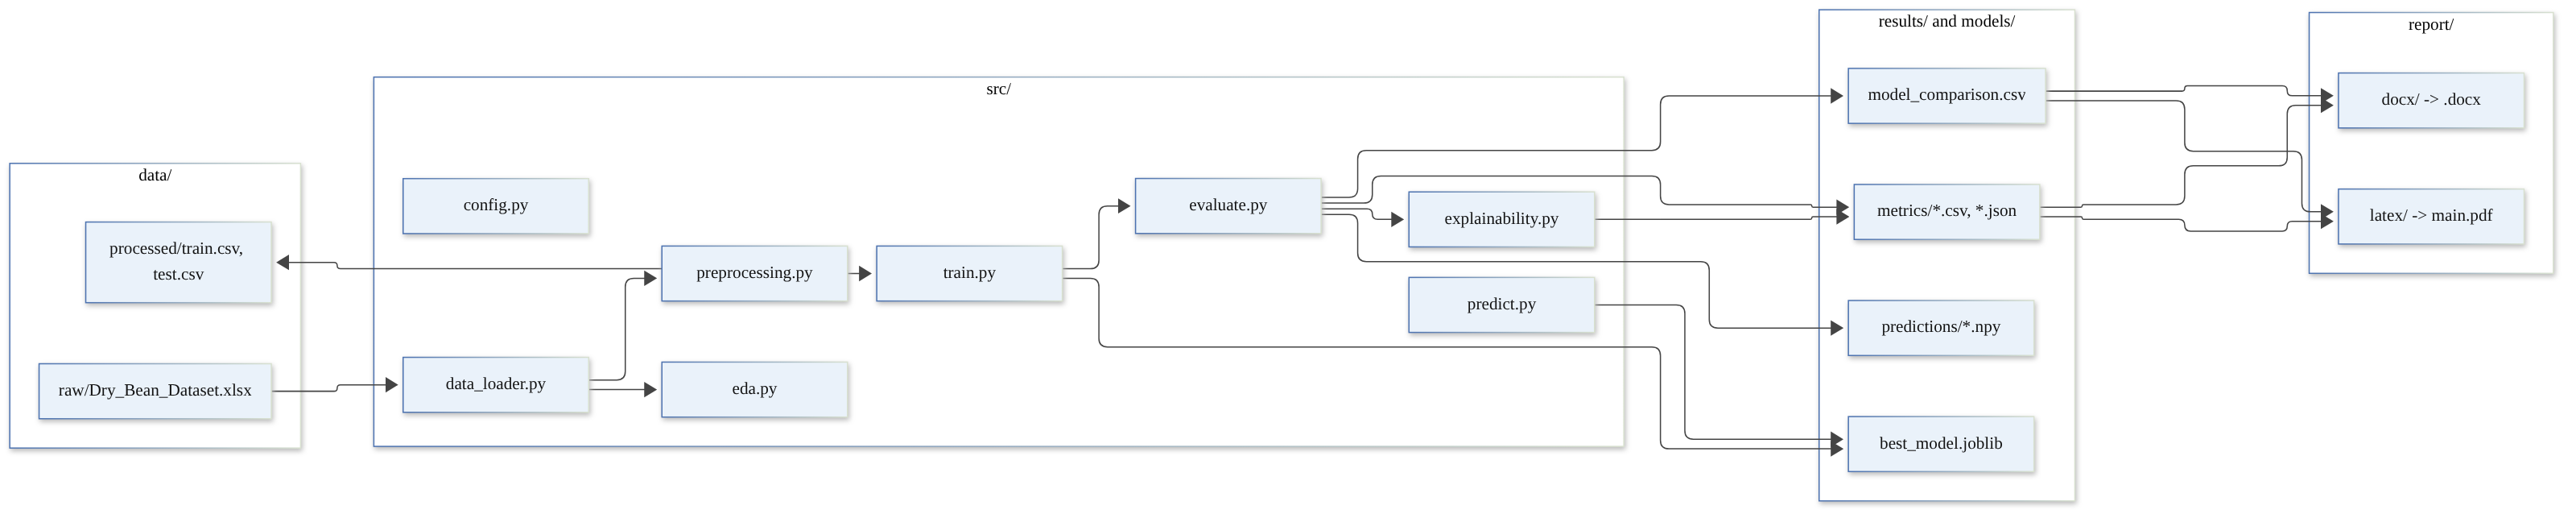
\includegraphics[width=\textwidth]{fig_5_3_architecture.png}
\caption{Module and artefact layout. The report is generated from the files in
\texttt{results/}, not typed from them.}
\label{fig:arch}
\end{figure}

\begin{verbatim}
dry-bean-classification/
├── data/
│   ├── raw/                  Dry_Bean_Dataset.xlsx (downloaded)
│   └── processed/            train.csv, test.csv
├── docs/                     departmental format, mermaid sources
├── figures/
│   ├── eda/                  Chapter 3 and 4 figures
│   ├── models/               Chapter 5 figures
│   └── evaluation/           Chapter 6 figures
├── models/                   six tuned pipelines, best_model.joblib
├── notebooks/                01-04, executed end to end
├── report/
│   ├── latex/                main.tex, chapters/, tables/, references.bib
│   ├── docx/                 Word build of the same content
│   └── final/                compiled PDF
├── results/
│   ├── metrics/              JSON and CSV metric tables
│   ├── predictions/          per-model test predictions
│   ├── model_comparison.csv
│   └── experiment_metadata.json
├── scripts/                  notebook, figure and report builders
├── src/                      pipeline modules
└── tests/                    pytest suite
\end{verbatim}

\section{Installation and Execution}

The pipeline requires Python 3.11 or newer and no GPU. From a clean checkout:

\begin{verbatim}
python3.12 -m venv .venv
source .venv/bin/activate
pip install -r requirements.txt

python -m src.run_pipeline        # download, validate, EDA, train, evaluate
pytest -q                         # 16 tests
jupyter nbconvert --execute --to notebook --inplace notebooks/*.ipynb
python -m src.predict --csv results/predictions/sample_predictions.csv
\end{verbatim}

The dataset is fetched automatically on the first run and cached in
\texttt{data/raw/}. If the machine is offline, placing
\texttt{Dry\_Bean\_Dataset.xlsx} in that directory is sufficient; the loader
skips the download when the file is present.

\section{Determinism}

Four mechanisms make the run reproducible. A single global seed
(\texttt{RANDOM\_STATE = 42}) is used for the split, for every cross-validation
splitter, for every stochastic estimator and for the randomised searches. The
split is written to disk and reloaded by every later stage, so the partition
cannot change between scripts. All searches are deterministic given the seed
because scikit-learn's randomised search draws from a seeded generator. Finally,
the report tables and the number macros in this document are generated from
\texttt{results/} by \texttt{scripts/build\_report\_assets.py}, so a re-run
updates the text rather than leaving stale figures behind.

\section{Key Code}

Listing~\ref{lst:search} shows the search construction. The pipeline, the
scoring rule and the splitter are fixed; only the estimator and its parameter
distribution vary between models.

\begin{lstlisting}[style=pycode, caption={Cross-validated search with the shared
protocol.}, label={lst:search}]
def _search(model_name, spec, split):
    pipe = build_pipeline(spec["estimator"], spec["scale"])
    kwargs = dict(estimator=pipe, scoring="f1_macro",
                  cv=StratifiedKFold(5, shuffle=True, random_state=42),
                  n_jobs=-1, refit=True)
    if spec["search"] == "grid":
        return GridSearchCV(param_grid=spec["params"], **kwargs)
    return RandomizedSearchCV(param_distributions=spec["params"],
                              n_iter=spec["n_iter"], random_state=42, **kwargs)
\end{lstlisting}

Listing~\ref{lst:validate} shows the integrity checks whose output fills
Table~\ref{tab:dataset_summary} and Section~4.1. Nothing is modified at this
stage, so the report can state exactly what was found before any cleaning
decision.

\begin{lstlisting}[style=pycode, caption={Validation reports facts; it never
cleans.}, label={lst:validate}]
def validate(df):
    feature_frame = df[FEATURES]
    corr = feature_frame.corr()
    upper = corr.where(np.triu(np.ones(corr.shape), k=1).astype(bool))
    return {
        "rows": int(df.shape[0]),
        "missing_values_total": int(df.isna().sum().sum()),
        "duplicate_rows": int(df.duplicated().sum()),
        "class_counts_ordered": {k: int((df[TARGET] == k).sum())
                                 for k in CLASS_ORDER},
        "feature_pairs_abs_corr_ge_0.90": {
            f"{a} ~ {b}": float(v)
            for (a, b), v in upper.stack().loc[lambda s: s.abs() >= 0.90].items()},
    }
\end{lstlisting}

\section{Test Suite}

Sixteen tests cover the three failure modes that matter for this project:
corrupted input, leakage, and a broken prediction path. The data tests assert the
verified shape, the absence of missing values, the seven labels and the exact
published class counts. The preprocessing tests assert the split size, that the
stratification holds to within 0.5 percentage points, that the split is
deterministic, that no row appears in both partitions, that the scaler's mean
equals the training mean, and that a standardised kNN is invariant to multiplying
every input by 100. The prediction tests assert that the saved model returns valid
labels, that the reported confidence is the top-3 maximum, that missing and
non-finite inputs are rejected, that the metadata agrees with the comparison table,
and that the command-line entry point returns success.

\chapter{ADDITIONAL RESULTS}

This appendix carries the material that supports the argument of Chapter~6 but is
too detailed for the main text: the fold-by-fold scores behind
Table~\ref{tab:cv_results}, the confusion counts behind
Table~\ref{tab:per_class}, the per-class ROC-AUC behind Figure~\ref{fig:roc}, and
the complete list of strongly correlated feature pairs.

\section{Cross-Validation Stability}

Table~\ref{tab:cv_folds} gives the macro F1 of the selected configuration in each
of the five folds. The spread is what makes the ranking in Table~\ref{tab:cv_results}
fragile: the fold-to-fold range of a single model is comparable to the gap between
adjacent models, so the middle of the leaderboard should not be read as a strict
ordering.

\begin{table}[htbp]
\centering
ootnotesize
\caption{Macro F1 of the selected configuration in each cross-validation fold}
\label{tab:cv_folds}
\begin{tabular}{lrrrrrrr}
\toprule
Model & Fold 1 & Fold 2 & Fold 3 & Fold 4 & Fold 5 & Mean & Std. dev. \\
\midrule
Logistic Regression & 0.9425 & 0.9423 & 0.9321 & 0.9337 & 0.9364 & 0.9374 & 0.0048 \\
K-Nearest Neighbours & 0.9397 & 0.9426 & 0.9324 & 0.9339 & 0.9424 & 0.9382 & 0.0048 \\
RBF-SVM & 0.9491 & 0.9516 & 0.9403 & 0.9391 & 0.9419 & 0.9444 & 0.0056 \\
Random Forest & 0.9364 & 0.9440 & 0.9354 & 0.9366 & 0.9352 & 0.9375 & 0.0037 \\
Extra Trees & 0.9340 & 0.9402 & 0.9332 & 0.9316 & 0.9330 & 0.9344 & 0.0033 \\
Hist Gradient Boosting & 0.9425 & 0.9506 & 0.9379 & 0.9402 & 0.9406 & 0.9424 & 0.0049 \\
\bottomrule
\end{tabular}
\end{table}


\section{Confusion Counts}

Table~\ref{tab:confusion_best} reproduces the counts behind the normalised matrix
in Figure~\ref{fig:cmbest}. Reading it by column rather than by row gives the
precision view: the Sira column receives 50 beans that are not Sira, which is why
its precision is lower than that of the other five large classes.

\begin{table}[htbp]
\centering
\scriptsize
\caption{Confusion matrix of the selected model (RBF-SVM) on the test set}
\label{tab:confusion_best}
\begin{tabular}{lrrrrrrrr}
\toprule
Actual \textbackslash{} Predicted & Seker & Barbunya & Bombay & Cali & Dermason & Horoz & Sira & Recall base \\
\midrule
Seker & 390 & 2 & 0 & 0 & 5 & 0 & 9 & 406 \\
Barbunya & 3 & 242 & 0 & 15 & 0 & 0 & 5 & 265 \\
Bombay & 0 & 0 & 104 & 0 & 0 & 0 & 0 & 104 \\
Cali & 2 & 11 & 0 & 305 & 0 & 6 & 2 & 326 \\
Dermason & 9 & 0 & 0 & 0 & 654 & 0 & 46 & 709 \\
Horoz & 0 & 2 & 0 & 5 & 5 & 367 & 7 & 386 \\
Sira & 8 & 3 & 0 & 0 & 51 & 6 & 459 & 527 \\
\midrule
Total & 412 & 260 & 104 & 325 & 715 & 379 & 528 & 2723 \\
\bottomrule
\end{tabular}
\end{table}


\section{Per-Class Ranking Quality}

Table~\ref{tab:roc_class} reports the one-vs-rest ROC-AUC per variety. Every class
exceeds 0.986, and Bombay reaches 1.000, which separates two different questions:
the model ranks beans of different varieties almost perfectly, but the single
threshold implied by \texttt{predict} still misassigns 7.42\% of them. A
rejection option built on the calibrated probability would exploit that gap.

\begin{table}[htbp]
\centering
\small
\caption{Per-class ROC-AUC of the selected model on the test set}
\label{tab:roc_class}
\begin{tabular}{lr}
\toprule
Variety & One-vs-rest ROC-AUC \\
\midrule
Seker & 0.9982 \\
Barbunya & 0.9959 \\
Bombay & 1.0000 \\
Cali & 0.9964 \\
Dermason & 0.9928 \\
Horoz & 0.9976 \\
Sira & 0.9862 \\
\bottomrule
\end{tabular}
\end{table}


\section{Complete Correlation Structure}

Table~\ref{tab:corr_all} lists all 21 feature pairs with $|r| \ge 0.90$. The
clustering is not random: it follows the algebra of the shape-factor definitions in
Equations~\eqref{eq:roundness}--\eqref{eq:zscore}. Any attribution of importance among the members of a cluster
is therefore arbitrary, as Section~6.7 states.

\begin{table}[htbp]
\centering
ootnotesize
\caption{All 21 feature pairs with $|r| \ge 0.90$}
\label{tab:corr_all}
\begin{tabular}{clr}
\toprule
No. & Feature pair & Pearson r \\
\midrule
1 & Area -- ConvexArea & +0.9999 \\
2 & Compactness -- ShapeFactor3 & +0.9987 \\
3 & Perimeter -- EquivDiameter & +0.9914 \\
4 & AspectRation -- Compactness & -0.9877 \\
5 & ConvexArea -- EquivDiameter & +0.9852 \\
6 & Area -- EquivDiameter & +0.9850 \\
7 & Eccentricity -- ShapeFactor3 & -0.9811 \\
8 & AspectRation -- ShapeFactor3 & -0.9786 \\
9 & Perimeter -- MajorAxisLength & +0.9773 \\
10 & Eccentricity -- Compactness & -0.9703 \\
11 & Perimeter -- ConvexArea & +0.9677 \\
12 & Area -- Perimeter & +0.9667 \\
13 & MajorAxisLength -- EquivDiameter & +0.9617 \\
14 & Area -- MinorAxisLength & +0.9516 \\
15 & MinorAxisLength -- ConvexArea & +0.9513 \\
16 & MinorAxisLength -- EquivDiameter & +0.9485 \\
17 & MinorAxisLength -- ShapeFactor1 & -0.9472 \\
18 & MajorAxisLength -- ConvexArea & +0.9326 \\
19 & Area -- MajorAxisLength & +0.9318 \\
20 & AspectRation -- Eccentricity & +0.9243 \\
21 & Perimeter -- MinorAxisLength & +0.9132 \\
\bottomrule
\end{tabular}
\end{table}



\end{document}
